\documentclass{article}\usepackage[]{graphicx}\usepackage[]{xcolor}
% maxwidth is the original width if it is less than linewidth
% otherwise use linewidth (to make sure the graphics do not exceed the margin)
\makeatletter
\def\maxwidth{ %
  \ifdim\Gin@nat@width>\linewidth
    \linewidth
  \else
    \Gin@nat@width
  \fi
}
\makeatother

\definecolor{fgcolor}{rgb}{0.345, 0.345, 0.345}
\newcommand{\hlnum}[1]{\textcolor[rgb]{0.686,0.059,0.569}{#1}}%
\newcommand{\hlstr}[1]{\textcolor[rgb]{0.192,0.494,0.8}{#1}}%
\newcommand{\hlcom}[1]{\textcolor[rgb]{0.678,0.584,0.686}{\textit{#1}}}%
\newcommand{\hlopt}[1]{\textcolor[rgb]{0,0,0}{#1}}%
\newcommand{\hlstd}[1]{\textcolor[rgb]{0.345,0.345,0.345}{#1}}%
\newcommand{\hlkwa}[1]{\textcolor[rgb]{0.161,0.373,0.58}{\textbf{#1}}}%
\newcommand{\hlkwb}[1]{\textcolor[rgb]{0.69,0.353,0.396}{#1}}%
\newcommand{\hlkwc}[1]{\textcolor[rgb]{0.333,0.667,0.333}{#1}}%
\newcommand{\hlkwd}[1]{\textcolor[rgb]{0.737,0.353,0.396}{\textbf{#1}}}%
\let\hlipl\hlkwb

\usepackage{framed}
\makeatletter
\newenvironment{kframe}{%
 \def\at@end@of@kframe{}%
 \ifinner\ifhmode%
  \def\at@end@of@kframe{\end{minipage}}%
  \begin{minipage}{\columnwidth}%
 \fi\fi%
 \def\FrameCommand##1{\hskip\@totalleftmargin \hskip-\fboxsep
 \colorbox{shadecolor}{##1}\hskip-\fboxsep
     % There is no \\@totalrightmargin, so:
     \hskip-\linewidth \hskip-\@totalleftmargin \hskip\columnwidth}%
 \MakeFramed {\advance\hsize-\width
   \@totalleftmargin\z@ \linewidth\hsize
   \@setminipage}}%
 {\par\unskip\endMakeFramed%
 \at@end@of@kframe}
\makeatother

\definecolor{shadecolor}{rgb}{.97, .97, .97}
\definecolor{messagecolor}{rgb}{0, 0, 0}
\definecolor{warningcolor}{rgb}{1, 0, 1}
\definecolor{errorcolor}{rgb}{1, 0, 0}
\newenvironment{knitrout}{}{} % an empty environment to be redefined in TeX

\usepackage{alltt}
\usepackage[italian]{babel}
\usepackage[T1]{fontenc}

\title{NMC - Foundations of Statistical Modelling}
\author{Lorenzo Baiardi}
\date{13 Aprile 2023}
\IfFileExists{upquote.sty}{\usepackage{upquote}}{}
\begin{document}

\maketitle

\clearpage

\tableofcontents

\clearpage


\section{Introduzione}
  In questo elaborato andremo a studiare l'effeto delle attività personali di un 
  individuo per la prevenzione di problemi cardiovascolari. Andremo a ipotizzare
  modelli specifici, differenze che si possono verificare tra le diverse categorie
  di persone e quanto queste categorie possono influire sulla presenza o meno
  di un problema cardiovascolare.


\section{Visualizzazione del dataset} 
  Per lo studio di questo fenomeno utilizzeremo il dataset fornito: 
  $\emph{Sjolander et al.(2009)}$ \par
  Il dataset fornisce un campione di numerosità: n = 33327 osservazioni. 
  
\begin{knitrout}
\definecolor{shadecolor}{rgb}{0.969, 0.969, 0.969}\color{fgcolor}\begin{kframe}
\begin{alltt}
\hlkwd{load}\hlstd{(}\hlstr{"../nmc.RData"}\hlstd{)}
\hlcom{#bmi dicotomizzata}
\hlstd{nmc}\hlopt{$}\hlstd{bmi} \hlkwb{=} \hlkwd{as.numeric}\hlstd{(nmc}\hlopt{$}\hlstd{bmi}\hlopt{>=}\hlnum{30}\hlstd{)}
\hlkwd{str}\hlstd{(nmc)}
\end{alltt}
\begin{verbatim}
## 'data.frame':	33327 obs. of  8 variables:
##  $ sex    : chr  "Male" "Female" "Male" "Female" ...
##  $ age    : int  94 93 92 92 91 90 89 89 89 89 ...
##  $ bmi    : num  0 0 0 0 0 0 0 0 1 0 ...
##  $ cvd    : int  0 0 0 1 0 0 0 1 0 1 ...
##  $ fitness: chr  "Just as good" "Much Worse" "A bit better" "Just as good" ...
##  $ pa     : int  0 1 1 0 0 0 0 0 0 0 ...
##  $ smoke  : chr  "NO" "NO" "Former" "Former" ...
##  $ alc    : chr  "Medium" "Low" "Never" "Never" ...
\end{verbatim}
\end{kframe}
\end{knitrout}
 
  \subsection{Variabili}
    \begin{itemize}
      \item CVD: variabile d'interesse.
        \begin{enumerate}
          \setcounter{enumi}{-1}
          \item Nessun problema cardiovascolare
          \item Uno o più problemi cardiovascolari
        \end{enumerate}
      \item Sex: rappresenta il genere dell'individuo.
        \begin{itemize}
          \item Male
          \item Female
        \end{itemize}
      \item Age: età dell'individuo.
      \item BMI: Body Mass Index, valore dicotomizzato.
        \begin{enumerate}
          \setcounter{enumi}{-1}
          \item BMI $< 30$
          \item BMI $\ge 30$ 
        \end{enumerate}
      \item Fitness: statico di salute dell'indiviudo.
        \begin{enumerate}
          \item Much Worse 
          \item Little Worse
          \item Just as good
          \item A bit better
          \item Much better
        \end{enumerate}
      \item PA: Personal Activities.
        \begin{enumerate}
          \setcounter{enumi}{-1}
          \item high-level exerciser 
          \item low-level exerciser
        \end{enumerate}
      \item Smoke: tipologia di fumatore.
        \begin{itemize}
          \item NO 
          \item Former
          \item Current
        \end{itemize}
      \item Alchol: frequenza nel consumo di alchol dell'individuo.
        \begin{enumerate}
          \item Never 
          \item Low
          \item Medium
          \item High
        \end{enumerate}
    \end{itemize}
  
    Per una maggiore comprensione del problema, convertiremo le variabili di
    tipo categoriale Fitness e Alchol, fornite dal dataset, in variabili di tipo        ordinale facilitando la valutazione di quest'ultime durante l'analisi. \par
    Di seguito mostreremo la legenda utilizzata.
    

    
\begin{knitrout}
\definecolor{shadecolor}{rgb}{0.969, 0.969, 0.969}\color{fgcolor}\begin{kframe}
\begin{alltt}
\hlcom{#LEGENDA:}
\hlcom{#Fitness: 1-MUCH WORSE, 2-LITTLE WORSE, 3-JUST AS GOOD, }
\hlcom{#         4-A BIT BETTER, 5-MUCH BETTER}
\hlcom{#Alchol: 1-NEVER, 2-LOW, 3-MEDIUM, 4-HIGH}

\hlstd{c.fit} \hlkwb{=} \hlkwd{c}\hlstd{(}\hlstr{'Much Worse'}\hlstd{,} \hlstr{'Little Worse'}\hlstd{,} \hlstr{'Just as good'}\hlstd{,}
            \hlstr{'A bit better'}\hlstd{,} \hlstr{'Much better'}\hlstd{)}
\hlstd{c.alc} \hlkwb{=}  \hlkwd{c}\hlstd{(}\hlstr{'Never'}\hlstd{,} \hlstr{'Low'}\hlstd{,} \hlstr{'Medium'}\hlstd{,} \hlstr{'High'}\hlstd{)}

\hlcom{#Variabili ordinali}
\hlstd{nmc}\hlopt{$}\hlstd{fitness} \hlkwb{=} \hlkwd{as.numeric}\hlstd{(}\hlkwd{ordered}\hlstd{(nmc}\hlopt{$}\hlstd{fitness, c.fit))}
\hlstd{nmc}\hlopt{$}\hlstd{alc} \hlkwb{=} \hlkwd{as.numeric}\hlstd{(}\hlkwd{ordered}\hlstd{(nmc}\hlopt{$}\hlstd{alc, c.alc))}

\hlkwd{str}\hlstd{(nmc)}
\end{alltt}
\begin{verbatim}
## 'data.frame':	33327 obs. of  8 variables:
##  $ sex    : chr  "Male" "Female" "Male" "Female" ...
##  $ age    : int  94 93 92 92 91 90 89 89 89 89 ...
##  $ bmi    : num  0 0 0 0 0 0 0 0 1 0 ...
##  $ cvd    : int  0 0 0 1 0 0 0 1 0 1 ...
##  $ fitness: num  3 1 4 3 4 4 4 4 4 4 ...
##  $ pa     : int  0 1 1 0 0 0 0 0 0 0 ...
##  $ smoke  : chr  "NO" "NO" "Former" "Former" ...
##  $ alc    : num  3 2 1 1 3 2 1 3 3 1 ...
\end{verbatim}
\end{kframe}
\end{knitrout}

  \subsection{Tabella delle Frequenze}
    Visualizziamo la frequenza delle varie categorie all'interno del dataset.
\begin{knitrout}
\definecolor{shadecolor}{rgb}{0.969, 0.969, 0.969}\color{fgcolor}\begin{kframe}
\begin{alltt}
\hlcom{#Tabella}
\hlkwd{ftable}\hlstd{(sex}\hlopt{+}\hlstd{bmi}\hlopt{+}\hlstd{pa} \hlopt{~} \hlstd{smoke}\hlopt{+}\hlstd{alc}\hlopt{+}\hlstd{fitness, nmc)}
\end{alltt}
\begin{verbatim}
##                     sex Female                Male               
##                     bmi      0         1         0         1     
##                     pa       0    1    0    1    0    1    0    1
## smoke   alc fitness                                              
## Current 1   1                4    1    1    0    2    1    0    1
##             2               11    6    6    0    3    2    2    0
##             3               31    1    3    0    8    2    1    0
##             4                6    1    0    0    3    0    0    0
##             5                5    0    0    0    4    0    0    0
##         2   1               26    8   12    3    6    3    4    2
##             2              166   44   25    9   26    6    2    1
##             3              449   37   21    1   94   10    5    1
##             4              193    4    8    1   52    1    1    0
##             5               55    0    2    0   18    1    0    0
##         3   1               11    8    6    2   10    6    2    1
##             2               74   21   16    3   49   15    2    2
##             3              287   32   14    3  156   24   11    0
##             4              200    8    5    0  129    4    3    0
##             5               49    0    2    0   32    0    0    0
##         4   1                0    0    0    2    0    2    0    0
##             2                4    1    0    0    5    0    1    0
##             3               12    3    1    0   17    0    1    0
##             4                9    1    1    0    7    0    1    0
##             5                8    0    0    0    6    1    0    0
## Former  1   1                2    4    6    3    2    2    0    1
##             2               16    5   10    2    7    4    0    2
##             3               83   14   17    1   42    1    6    0
##             4               63    0    8    0   32    5    3    0
##             5               35    0    0    0   15    0    0    0
##         2   1               35   18   17   12    9    8    8    4
##             2              185   41   70   12   39   16   12    3
##             3             1005   70  124    8  279   40   27    5
##             4              799   24   33    0  348   14   16    0
##             5              290    1    3    1  140    0    4    1
##         3   1               11    7    9    8    9    5    6    5
##             2              132   26   27    8   94   34   30   14
##             3              846   81   57    6  563   57   47   11
##             4              829   15   22    2  740   24   34    2
##             5              281    2    3    0  308    2    6    0
##         4   1                3    0    0    0    2    1    0    0
##             2                4    0    0    0    3    2    0    0
##             3               39    2    3    0   45    7    6    2
##             4               28    2    1    0   60    2    5    0
##             5               14    0    0    0   24    0    0    0
## NO      1   1               30   13   21   10   10    3    1    1
##             2              209   38   49   10   68   22   10    1
##             3             1024   83  111    9  272   30   15    1
##             4              704   19   44    0  386   21    6    1
##             5              255    1    9    0  194    4    2    0
##         2   1               81   28   38   13   29    8    9    6
##             2              624  132  139   20  192   55   26   14
##             3             3169  258  246   18  805   92   48    4
##             4             2549   49   80    3 1059   36   19    1
##             5              876    6   21    0  628   12    3    1
##         3   1               24    9   14    4   21   10    7    3
##             2              212   42   41    9  124   48   23    5
##             3             1288  109   82   11  715  101   40    9
##             4             1326   29   36    2 1093   35   29    0
##             5              441    4    4    0  577    6    6    0
##         4   1                3    0    0    0    3    2    0    0
##             2                1    2    2    0    9    5    4    0
##             3               35    5    2    0   45    5    5    0
##             4               48    0    1    0   53    6    4    0
##             5               14    0    0    0   47    0    1    0
\end{verbatim}
\end{kframe}
\end{knitrout}
    
\clearpage


\section{Regressioni Logistiche Semplici}
  Dato che stiamo analizzando un problema che presenta come variabile di 
  risposta una varibile binaria (CVD), utilizzeremo la regressione logistica, 
  implementata in R tramite la funzione glm(). \par
  Per prima cosa analizzeremo le regressioni logistiche semplici delle singole
  variabili presenti nel dataset, visualizzandone il loro comportamento verso la
  nostra variabile di risposta.
  
  \subsection{Age}
\begin{knitrout}
\definecolor{shadecolor}{rgb}{0.969, 0.969, 0.969}\color{fgcolor}\begin{kframe}
\begin{alltt}
\hlcom{#Age}
\hlstd{fit.age} \hlkwb{<-} \hlkwd{glm}\hlstd{(nmc}\hlopt{$}\hlstd{cvd} \hlopt{~} \hlstd{nmc}\hlopt{$}\hlstd{age,} \hlkwc{family}\hlstd{=binomial)}
\hlkwd{summary}\hlstd{(fit.age)}
\end{alltt}
\begin{verbatim}
## 
## Call:
## glm(formula = nmc$cvd ~ nmc$age, family = binomial)
## 
## Deviance Residuals: 
##     Min       1Q   Median       3Q      Max  
## -1.3868  -0.3530  -0.2052  -0.0986   3.5606  
## 
## Coefficients:
##              Estimate Std. Error z value Pr(>|z|)    
## (Intercept) -8.179700   0.151662  -53.93   <2e-16 ***
## nmc$age      0.092122   0.002345   39.28   <2e-16 ***
## ---
## Signif. codes:  0 '***' 0.001 '**' 0.01 '*' 0.05 '.' 0.1 ' ' 1
## 
## (Dispersion parameter for binomial family taken to be 1)
## 
##     Null deviance: 13400  on 33326  degrees of freedom
## Residual deviance: 11150  on 33325  degrees of freedom
## AIC: 11154
## 
## Number of Fisher Scoring iterations: 7
\end{verbatim}
\end{kframe}
\end{knitrout}
    
    \begin{itemize}
      \item L'età influenza positivamente l'insorgenza di un problema 
            cardiovascolare, con valore stimato: Age $\sim$ 0.092. 
      \item La variabile Age è molto significativa secondo il \emph{p-value}.
    \end{itemize}
    
    Stampiamo ora il boxplot per valutare l'età delle persone che presentano
    o meno un problema cardiovascolare.
    
\begin{knitrout}
\definecolor{shadecolor}{rgb}{0.969, 0.969, 0.969}\color{fgcolor}\begin{kframe}
\begin{alltt}
\hlcom{#Boxplot}
\hlkwd{boxplot}\hlstd{(nmc}\hlopt{$}\hlstd{age}\hlopt{~}\hlstd{nmc}\hlopt{$}\hlstd{cvd,} \hlkwc{xlab}\hlstd{=}\hlstr{"CVD"}\hlstd{,} \hlkwc{ylab}\hlstd{=}\hlstr{"Age"}\hlstd{)}
\end{alltt}
\end{kframe}
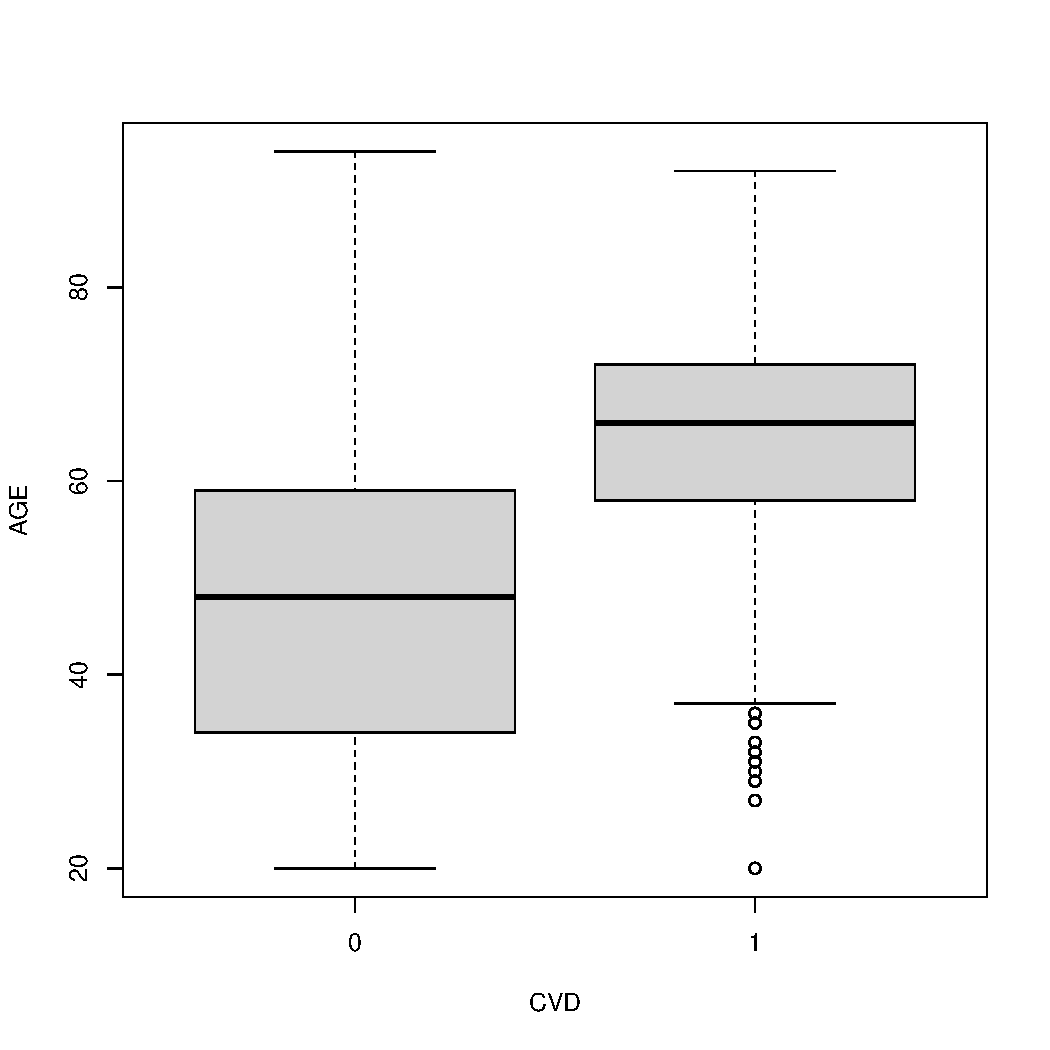
\includegraphics[width=\maxwidth]{figure/RLS_Age_BoxPlot-1} 
\end{knitrout}
    
    \begin{itemize}
      \item Il boxplot ci mostra come la media delle persone che hanno problemi
            cardiovascolari, all'interno del dataset, è quella della fascia
            tra i 60 e 80 anni.
      \item La media delle persone che non hanno un problema cardiovascolare è
            quella tra i 40 e 60 anni.
      \item I problemi cardiovascolari sono più frequenti nella fascia anziana
            della popolazione.
    \end{itemize}
    
    Eseguiamo il plot del modello con la sola variabile Age.\par
    Modello: CVD $\sim$ Age.
    
\begin{knitrout}
\definecolor{shadecolor}{rgb}{0.969, 0.969, 0.969}\color{fgcolor}\begin{kframe}
\begin{alltt}
\hlcom{#Plot}
\hlstd{pstima.age} \hlkwb{<-} \hlstd{fit.age}\hlopt{$}\hlstd{fitted.values}
\hlkwd{plot}\hlstd{(nmc}\hlopt{$}\hlstd{age, nmc}\hlopt{$}\hlstd{cvd,} \hlkwc{xlab}\hlstd{=}\hlstr{"Age"}\hlstd{,} \hlkwc{ylab}\hlstd{=}\hlstr{"CVD"}\hlstd{)}
\hlkwd{lines}\hlstd{(}\hlkwd{sort}\hlstd{(nmc}\hlopt{$}\hlstd{age), pstima.age[}\hlkwd{order}\hlstd{(nmc}\hlopt{$}\hlstd{age)],} \hlkwc{col}\hlstd{=}\hlstr{"blue"}\hlstd{)}
\end{alltt}
\end{kframe}
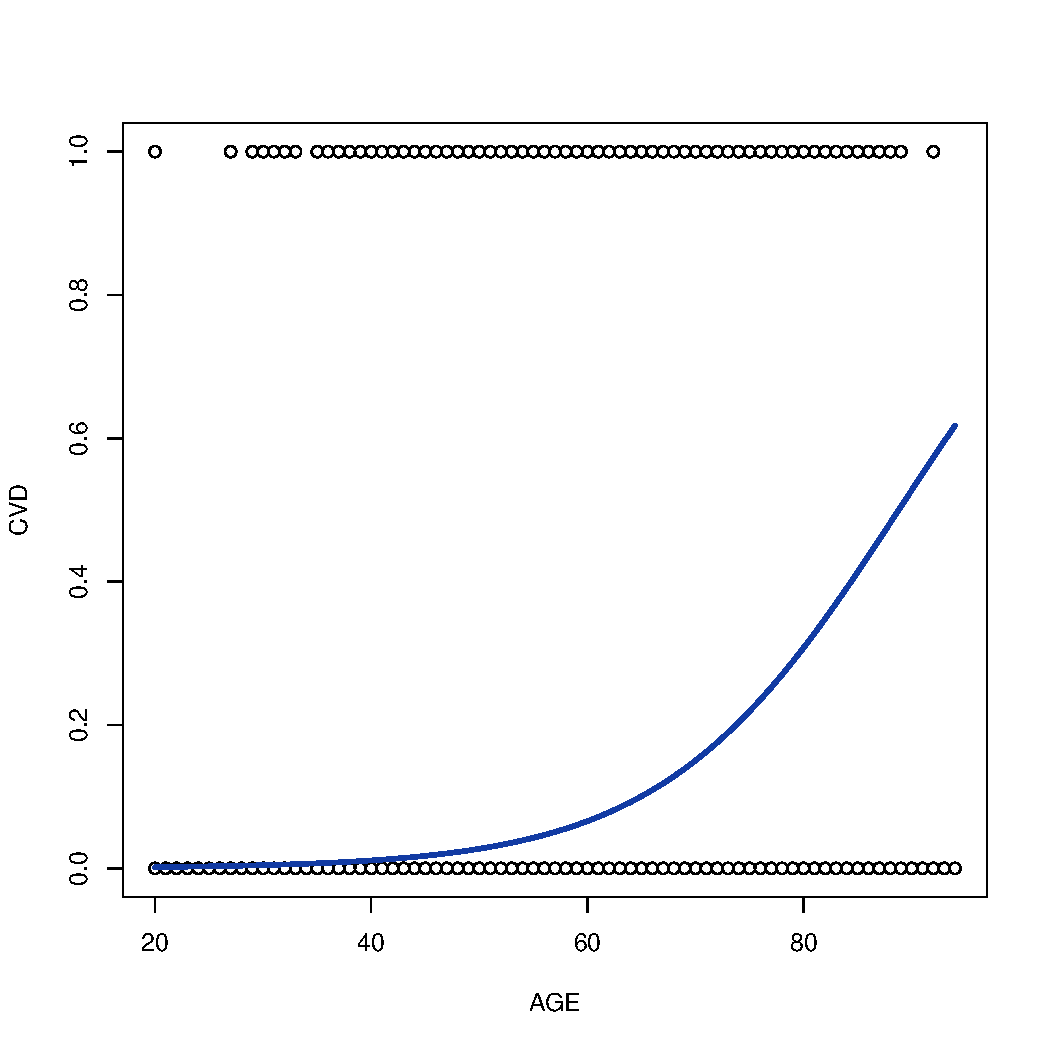
\includegraphics[width=\maxwidth]{figure/RLS_Age_Plot-1} 
\end{knitrout}
    
    Il modello e il grafico suggeriscono come, all'aumentare dell'età, ci sia un 
    aumento esponenziale nelle probabilità nell'incorrere in un problema 
    cardiovascolare. In particolare possiamo notare, come visulizzato anche dal
    boxplot, che superata la soglia dei 40 anni si ha un notevole aumento nella
    probabilità di CVD, confermando quindi come questo problema sia legato
    principalmente ad un fattore di età.
  
  \clearpage
  
  \subsection{Sex}
\begin{knitrout}
\definecolor{shadecolor}{rgb}{0.969, 0.969, 0.969}\color{fgcolor}\begin{kframe}
\begin{alltt}
\hlcom{#Regressioni logistiche semplici}
\hlcom{#Sex}
\hlstd{fit.sex} \hlkwb{<-} \hlkwd{glm}\hlstd{(nmc}\hlopt{$}\hlstd{cvd} \hlopt{~} \hlstd{nmc}\hlopt{$}\hlstd{sex,} \hlkwc{family}\hlstd{=binomial)}
\hlkwd{summary}\hlstd{(fit.sex)}
\end{alltt}
\begin{verbatim}
## 
## Call:
## glm(formula = nmc$cvd ~ nmc$sex, family = binomial)
## 
## Deviance Residuals: 
##     Min       1Q   Median       3Q      Max  
## -0.4152  -0.4152  -0.2668  -0.2668   2.5898  
## 
## Coefficients:
##             Estimate Std. Error z value Pr(>|z|)    
## (Intercept) -3.31797    0.03654  -90.80   <2e-16 ***
## nmc$sexMale  0.91004    0.05021   18.12   <2e-16 ***
## ---
## Signif. codes:  0 '***' 0.001 '**' 0.01 '*' 0.05 '.' 0.1 ' ' 1
## 
## (Dispersion parameter for binomial family taken to be 1)
## 
##     Null deviance: 13400  on 33326  degrees of freedom
## Residual deviance: 13073  on 33325  degrees of freedom
## AIC: 13077
## 
## Number of Fisher Scoring iterations: 6
\end{verbatim}
\end{kframe}
\end{knitrout}
    
    \begin{itemize}
      \item Nella regressione logistica semplice, il sesso Maschile 
            sembra aumentare notevolmente la possibilità di incorrere in un CVD 
            rispetto al sesso Femminile, con valore stimato: 
            SexMale $\sim$ 0.910.
      \item La variabile Sex risulta molto significativa secondo il \emph{p-value}, 
            superando quindi il $5\%$ di significatività.
    \end{itemize}
    
    Valutiamo quanto il sesso possa influire nella presenza o meno di CVD.
    
\begin{knitrout}
\definecolor{shadecolor}{rgb}{0.969, 0.969, 0.969}\color{fgcolor}\begin{kframe}
\begin{alltt}
\hlcom{#Modello per Maschio}
\hlstd{fit.sex.male} \hlkwb{<-} \hlkwd{glm}\hlstd{(nmc}\hlopt{$}\hlstd{cvd[nmc}\hlopt{$}\hlstd{sex}\hlopt{==}\hlstr{"Male"}\hlstd{]} \hlopt{~}
                      \hlstd{nmc}\hlopt{$}\hlstd{age[nmc}\hlopt{$}\hlstd{sex}\hlopt{==}\hlstr{"Male"}\hlstd{],}
                      \hlkwc{family}\hlstd{=binomial)}
\hlstd{pstima.sex.male} \hlkwb{<-} \hlstd{fit.sex.male}\hlopt{$}\hlstd{fitted.values}
\hlcom{#Modello per Femmina}
\hlstd{fit.sex.female} \hlkwb{<-} \hlkwd{glm}\hlstd{(nmc}\hlopt{$}\hlstd{cvd[nmc}\hlopt{$}\hlstd{sex}\hlopt{==}\hlstr{"Female"}\hlstd{]} \hlopt{~}
                        \hlstd{nmc}\hlopt{$}\hlstd{age[nmc}\hlopt{$}\hlstd{sex}\hlopt{==}\hlstr{"Female"}\hlstd{],}
                        \hlkwc{family}\hlstd{=binomial)}
\hlstd{pstima.sex.female} \hlkwb{<-} \hlstd{fit.sex.female}\hlopt{$}\hlstd{fitted.values}
\hlcom{#Plot}
\hlkwd{plot}\hlstd{(nmc}\hlopt{$}\hlstd{age[nmc}\hlopt{$}\hlstd{sex}\hlopt{==}\hlstr{"Male"}\hlstd{], nmc}\hlopt{$}\hlstd{cvd[nmc}\hlopt{$}\hlstd{sex}\hlopt{==}\hlstr{"Male"}\hlstd{],}
     \hlkwc{xlab}\hlstd{=}\hlstr{"Age"}\hlstd{,} \hlkwc{ylab}\hlstd{=}\hlstr{"CVD"}\hlstd{,} \hlkwc{col}\hlstd{=}\hlstr{"blue"}\hlstd{)}
\hlkwd{points}\hlstd{(nmc}\hlopt{$}\hlstd{age[nmc}\hlopt{$}\hlstd{sex}\hlopt{==}\hlstr{"Female"}\hlstd{], nmc}\hlopt{$}\hlstd{cvd[nmc}\hlopt{$}\hlstd{sex}\hlopt{==}\hlstr{"Female"}\hlstd{],}
       \hlkwc{col}\hlstd{=}\hlstr{"red"}\hlstd{)}
\hlkwd{lines}\hlstd{(nmc}\hlopt{$}\hlstd{age[nmc}\hlopt{$}\hlstd{sex}\hlopt{==}\hlstr{"Male"}\hlstd{], pstima.sex.male,} \hlkwc{col}\hlstd{=}\hlstr{"blue"}\hlstd{)}
\hlkwd{lines}\hlstd{(nmc}\hlopt{$}\hlstd{age[nmc}\hlopt{$}\hlstd{sex}\hlopt{==}\hlstr{"Female"}\hlstd{], pstima.sex.female,} \hlkwc{col}\hlstd{=}\hlstr{"red"}\hlstd{)}
\hlkwd{legend}\hlstd{(}\hlkwc{x}\hlstd{=}\hlstr{"left"}\hlstd{,} \hlkwc{legend}\hlstd{=}\hlkwd{c}\hlstd{(}\hlstr{"Male"}\hlstd{,} \hlstr{"Female"}\hlstd{),} \hlkwc{lty}\hlstd{=}\hlkwd{c}\hlstd{(}\hlnum{1}\hlstd{,} \hlnum{1}\hlstd{),}
       \hlkwc{col}\hlstd{=}\hlkwd{c}\hlstd{(}\hlstr{"blue"}\hlstd{,}\hlstr{"red"}\hlstd{),} \hlkwc{lwd}\hlstd{=}\hlnum{1}\hlstd{)}
\end{alltt}
\end{kframe}
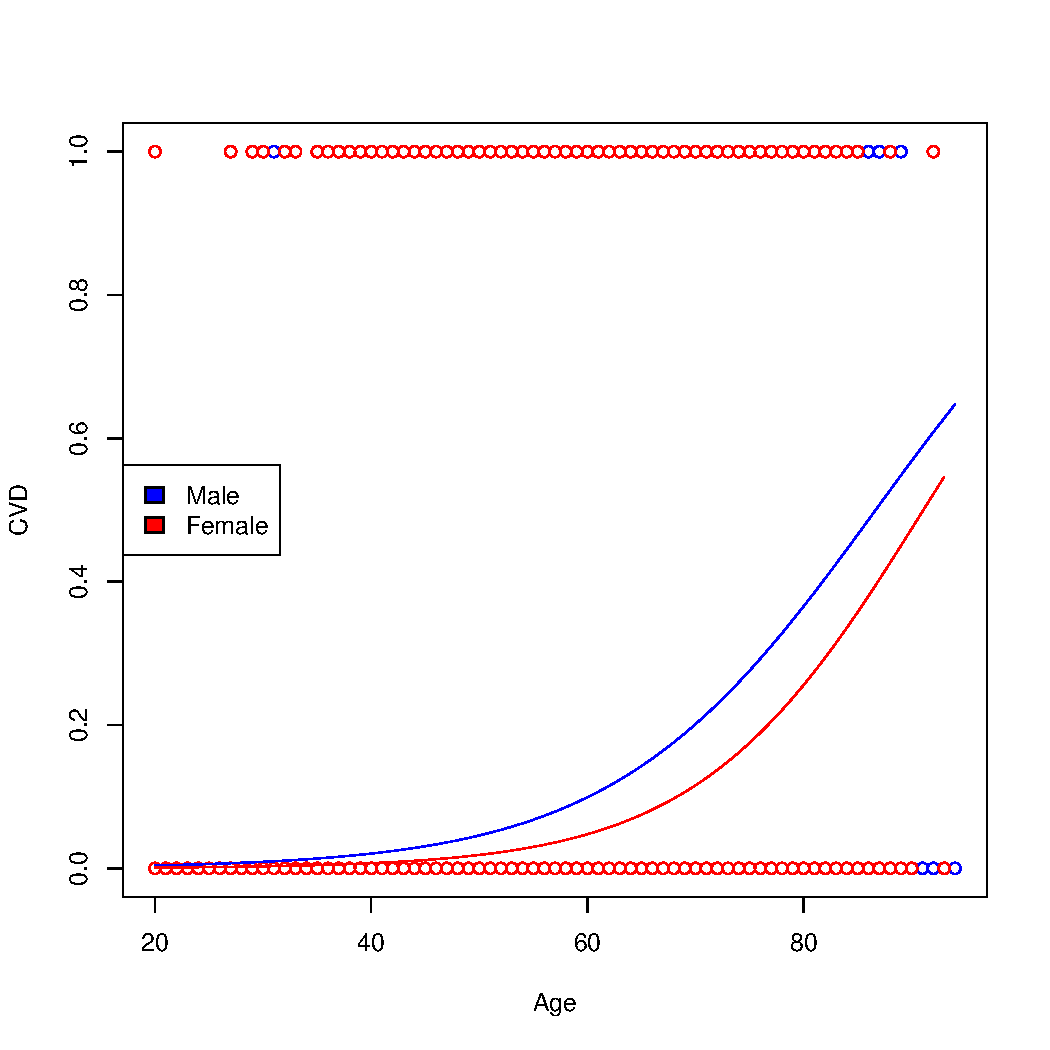
\includegraphics[width=\maxwidth]{figure/RLS_Sex_Plot-1} 
\end{knitrout}
  
    Il grafico ci conferma come il sesso maschile sia più a rischio di problemi
    cardiovascolari rispetto al sesso femminile.
  
  \subsection{BMI}
\begin{knitrout}
\definecolor{shadecolor}{rgb}{0.969, 0.969, 0.969}\color{fgcolor}\begin{kframe}
\begin{alltt}
\hlcom{#BMI}
\hlstd{fit.bmi} \hlkwb{<-} \hlkwd{glm}\hlstd{(nmc}\hlopt{$}\hlstd{cvd} \hlopt{~} \hlstd{nmc}\hlopt{$}\hlstd{bmi,} \hlkwc{family}\hlstd{=binomial)}
\hlkwd{summary}\hlstd{(fit.bmi)}
\end{alltt}
\begin{verbatim}
## 
## Call:
## glm(formula = nmc$cvd ~ nmc$bmi, family = binomial)
## 
## Deviance Residuals: 
##     Min       1Q   Median       3Q      Max  
## -0.3614  -0.3201  -0.3201  -0.3201   2.4481  
## 
## Coefficients:
##             Estimate Std. Error  z value Pr(>|z|)    
## (Intercept) -2.94542    0.02605 -113.070  < 2e-16 ***
## nmc$bmi      0.24948    0.08995    2.773  0.00555 ** 
## ---
## Signif. codes:  0 '***' 0.001 '**' 0.01 '*' 0.05 '.' 0.1 ' ' 1
## 
## (Dispersion parameter for binomial family taken to be 1)
## 
##     Null deviance: 13400  on 33326  degrees of freedom
## Residual deviance: 13393  on 33325  degrees of freedom
## AIC: 13397
## 
## Number of Fisher Scoring iterations: 5
\end{verbatim}
\end{kframe}
\end{knitrout}
    
    \begin{itemize}
      \item La variabile BMI risulta positiva nell'insorgenza di un CVD con 
            valore stimato: BMI $\sim$ 0.249.
      \item La variabile BMI risulta significativa secondo il \emph{p-value}.
    \end{itemize}
    
    Visualizziamo come il BMI possa influenzare nell'avanzamento dell'età.
    
\begin{knitrout}
\definecolor{shadecolor}{rgb}{0.969, 0.969, 0.969}\color{fgcolor}\begin{kframe}
\begin{alltt}
\hlcom{#BMI 0}
\hlstd{fit.bmi.0} \hlkwb{<-} \hlkwd{glm}\hlstd{(nmc}\hlopt{$}\hlstd{cvd[nmc}\hlopt{$}\hlstd{bmi}\hlopt{==}\hlnum{0}\hlstd{]} \hlopt{~} \hlstd{nmc}\hlopt{$}\hlstd{age[nmc}\hlopt{$}\hlstd{bmi}\hlopt{==}\hlnum{0}\hlstd{],}
                 \hlkwc{family}\hlstd{=binomial)}
\hlstd{pstima.bmi.0} \hlkwb{<-} \hlstd{fit.bmi.0}\hlopt{$}\hlstd{fitted.values}

\hlcom{#BMI 1}
\hlstd{fit.bmi.1} \hlkwb{<-} \hlkwd{glm}\hlstd{(nmc}\hlopt{$}\hlstd{cvd[nmc}\hlopt{$}\hlstd{bmi}\hlopt{==}\hlnum{1}\hlstd{]} \hlopt{~} \hlstd{nmc}\hlopt{$}\hlstd{age[nmc}\hlopt{$}\hlstd{bmi}\hlopt{==}\hlnum{1}\hlstd{],}
                 \hlkwc{family}\hlstd{=binomial)}
\hlstd{pstima.bmi.1} \hlkwb{<-} \hlstd{fit.bmi.1}\hlopt{$}\hlstd{fitted.values}

\hlcom{#Plot}
\hlkwd{plot}\hlstd{(nmc}\hlopt{$}\hlstd{age[nmc}\hlopt{$}\hlstd{bmi}\hlopt{==}\hlnum{0}\hlstd{], nmc}\hlopt{$}\hlstd{cvd[nmc}\hlopt{$}\hlstd{bmi}\hlopt{==}\hlnum{0}\hlstd{],}
     \hlkwc{xlab}\hlstd{=}\hlstr{"Age"}\hlstd{,} \hlkwc{ylab}\hlstd{=}\hlstr{"CVD"}\hlstd{,} \hlkwc{col}\hlstd{=}\hlstr{"blue"}\hlstd{)}
\hlkwd{points}\hlstd{(nmc}\hlopt{$}\hlstd{age[nmc}\hlopt{$}\hlstd{bmi}\hlopt{==}\hlnum{1}\hlstd{], nmc}\hlopt{$}\hlstd{cvd[nmc}\hlopt{$}\hlstd{bmi}\hlopt{==}\hlnum{1}\hlstd{],} \hlkwc{col}\hlstd{=}\hlstr{"red"}\hlstd{)}
\hlkwd{lines}\hlstd{(nmc}\hlopt{$}\hlstd{age[nmc}\hlopt{$}\hlstd{bmi}\hlopt{==}\hlnum{0}\hlstd{], pstima.bmi.0,} \hlkwc{col}\hlstd{=}\hlstr{"blue"}\hlstd{)}
\hlkwd{lines}\hlstd{(nmc}\hlopt{$}\hlstd{age[nmc}\hlopt{$}\hlstd{bmi}\hlopt{==}\hlnum{1}\hlstd{], pstima.bmi.1,} \hlkwc{col}\hlstd{=}\hlstr{"red"}\hlstd{)}
\hlkwd{legend}\hlstd{(}\hlkwc{x}\hlstd{=}\hlstr{"left"}\hlstd{,} \hlkwc{legend}\hlstd{=}\hlkwd{c}\hlstd{(}\hlstr{"BMI < 30"}\hlstd{,} \hlstr{"BMI >= 30"}\hlstd{),} \hlkwc{lty}\hlstd{=}\hlkwd{c}\hlstd{(}\hlnum{1}\hlstd{,} \hlnum{1}\hlstd{),}
       \hlkwc{col}\hlstd{=}\hlkwd{c}\hlstd{(}\hlstr{"blue"}\hlstd{,}\hlstr{"red"}\hlstd{),} \hlkwc{lwd}\hlstd{=}\hlnum{1}\hlstd{)}
\end{alltt}
\end{kframe}
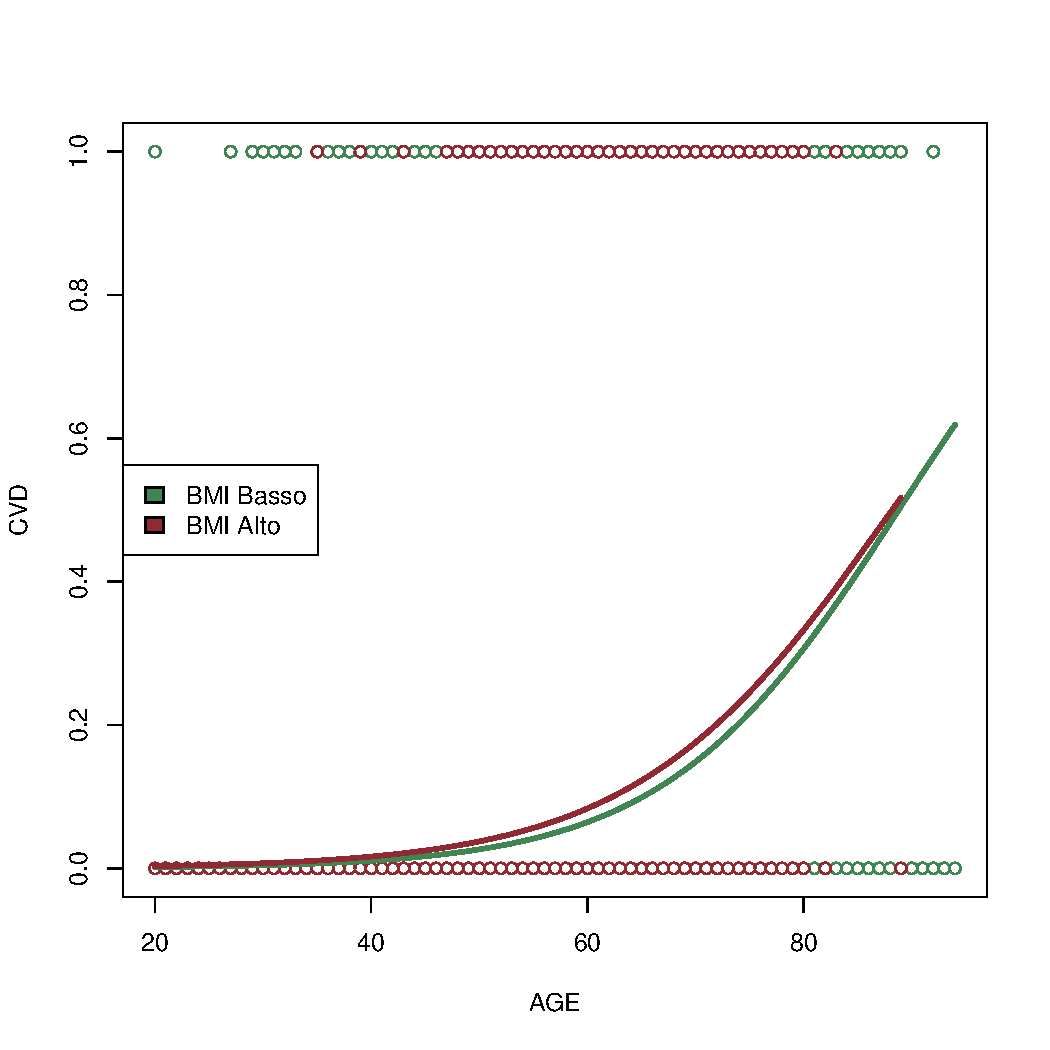
\includegraphics[width=\maxwidth]{figure/RLS_BMI_Plot-1} 
\end{knitrout}
  
    Le due curve sono molto simili tra di loro, con un leggero aumento per coloro
    che hanno un indice di massa corporea maggiore di 30.
    
  \clearpage
  
  \subsection{Fitness}
\begin{knitrout}
\definecolor{shadecolor}{rgb}{0.969, 0.969, 0.969}\color{fgcolor}\begin{kframe}
\begin{alltt}
\hlcom{#Fitness}
\hlstd{fit.fitness} \hlkwb{<-} \hlkwd{glm}\hlstd{(nmc}\hlopt{$}\hlstd{cvd} \hlopt{~} \hlstd{nmc}\hlopt{$}\hlstd{fitness,} \hlkwc{family}\hlstd{=binomial)}
\hlkwd{summary}\hlstd{(fit.fitness)}
\end{alltt}
\begin{verbatim}
## 
## Call:
## glm(formula = nmc$cvd ~ nmc$fitness, family = binomial)
## 
## Deviance Residuals: 
##     Min       1Q   Median       3Q      Max  
## -0.3438  -0.3299  -0.3166  -0.3166   2.5218  
## 
## Coefficients:
##             Estimate Std. Error z value Pr(>|z|)    
## (Intercept) -3.22195    0.09918 -32.487   <2e-16 ***
## nmc$fitness  0.08459    0.02723   3.106   0.0019 ** 
## ---
## Signif. codes:  0 '***' 0.001 '**' 0.01 '*' 0.05 '.' 0.1 ' ' 1
## 
## (Dispersion parameter for binomial family taken to be 1)
## 
##     Null deviance: 13400  on 33326  degrees of freedom
## Residual deviance: 13390  on 33325  degrees of freedom
## AIC: 13394
## 
## Number of Fisher Scoring iterations: 5
\end{verbatim}
\end{kframe}
\end{knitrout}
    
    Contrariamente a quello che ci si potesse aspettare, per il solo modello di 
    regressione logistica semplice, la variabile ordinale Fitness risulta, anche
    se di poco, positiva e significativa per l'insorgenza di un problema 
    cardiovascolare. \par
    Verifichiamo quindi se ci siano delle differenze nel modello di regressione         logistica semplice 
    con la variabile categoriale di Fitness.
    
\begin{knitrout}
\definecolor{shadecolor}{rgb}{0.969, 0.969, 0.969}\color{fgcolor}\begin{kframe}
\begin{alltt}
\hlcom{#Fitness: Categoriale}
\hlstd{fit.fitness.cat} \hlkwb{<-} \hlkwd{glm}\hlstd{(nmc}\hlopt{$}\hlstd{cvd} \hlopt{~} \hlstd{fitness,} \hlkwc{family}\hlstd{=binomial)}
\hlkwd{summary}\hlstd{(fit.fitness.cat)}
\end{alltt}
\begin{verbatim}
## 
## Call:
## glm(formula = nmc$cvd ~ fitness, family = binomial)
## 
## Deviance Residuals: 
##     Min       1Q   Median       3Q      Max  
## -0.3404  -0.3404  -0.3083  -0.3083   2.4894  
## 
## Coefficients:
##                     Estimate Std. Error z value Pr(>|z|)    
## (Intercept)         -2.81935    0.04066 -69.344  < 2e-16 ***
## fitnessJust as good -0.20312    0.05783  -3.512 0.000444 ***
## fitnessLittle Worse -0.23313    0.09169  -2.542 0.011009 *  
## fitnessMuch better  -0.03049    0.07762  -0.393 0.694406    
## fitnessMuch Worse   -0.09915    0.17360  -0.571 0.567914    
## ---
## Signif. codes:  0 '***' 0.001 '**' 0.01 '*' 0.05 '.' 0.1 ' ' 1
## 
## (Dispersion parameter for binomial family taken to be 1)
## 
##     Null deviance: 13400  on 33326  degrees of freedom
## Residual deviance: 13384  on 33322  degrees of freedom
## AIC: 13394
## 
## Number of Fisher Scoring iterations: 5
\end{verbatim}
\end{kframe}
\end{knitrout}
    
    \begin{itemize}
      \item Con la variabile categoriale di Fitness notiamo come ci sia una 
            diminuzione nell'insorgenza di CVD per tutte le categorie.
      \item Solamente le categorie Fitness:Just as good e Fitness:Little Worse                  risultano significative.
    \end{itemize}
    
    Visulizziamo il comportamento della variabile Fitness all'aumentare dell'età.
    
\begin{knitrout}
\definecolor{shadecolor}{rgb}{0.969, 0.969, 0.969}\color{fgcolor}\begin{kframe}
\begin{alltt}
\hlcom{#Fitness Much Worse}
\hlstd{fit.fitness.muchworse} \hlkwb{<-} \hlkwd{glm}\hlstd{(nmc}\hlopt{$}\hlstd{cvd[fitness}\hlopt{==}\hlstr{"Much Worse"}\hlstd{]} \hlopt{~}
                               \hlstd{nmc}\hlopt{$}\hlstd{age[fitness}\hlopt{==}\hlstr{"Much Worse"}\hlstd{],}
                               \hlkwc{family}\hlstd{=binomial)}
\hlstd{pstima.fitness.muchworse} \hlkwb{<-} \hlstd{fit.fitness.muchworse}\hlopt{$}\hlstd{fitted.values}

\hlcom{#Fitness LittleWorse}
\hlstd{fit.fitness.littleworse} \hlkwb{<-} \hlkwd{glm}\hlstd{(nmc}\hlopt{$}\hlstd{cvd[fitness}\hlopt{==}\hlstr{"Little Worse"}\hlstd{]} \hlopt{~}
                                 \hlstd{nmc}\hlopt{$}\hlstd{age[fitness}\hlopt{==}\hlstr{"Little Worse"}\hlstd{],}
                                 \hlkwc{family}\hlstd{=binomial)}
\hlstd{pstima.fitness.littleworse} \hlkwb{<-} \hlstd{fit.fitness.littleworse}\hlopt{$}\hlstd{fitted.values}

\hlcom{#Fitness Just as good}
\hlstd{fit.fitness.justasgood}\hlkwb{<-} \hlkwd{glm}\hlstd{(nmc}\hlopt{$}\hlstd{cvd[fitness}\hlopt{==}\hlstr{"Just as good"}\hlstd{]} \hlopt{~}
                               \hlstd{nmc}\hlopt{$}\hlstd{age[fitness}\hlopt{==}\hlstr{"Just as good"}\hlstd{],}
                               \hlkwc{family}\hlstd{=binomial)}
\hlstd{pstima.fitness.justasgood} \hlkwb{<-} \hlstd{fit.fitness.justasgood}\hlopt{$}\hlstd{fitted.values}

\hlcom{#Fitness A bit better}
\hlstd{fit.fitness.abitbetter} \hlkwb{<-} \hlkwd{glm}\hlstd{(nmc}\hlopt{$}\hlstd{cvd[fitness}\hlopt{==}\hlstr{"A bit better"}\hlstd{]} \hlopt{~}
                                \hlstd{nmc}\hlopt{$}\hlstd{age[fitness}\hlopt{==}\hlstr{"A bit better"}\hlstd{],}
                                \hlkwc{family}\hlstd{=binomial)}
\hlstd{pstima.fitness.abitbetter} \hlkwb{<-} \hlstd{fit.fitness.abitbetter}\hlopt{$}\hlstd{fitted.values}

\hlcom{#Fitness Much better}
\hlstd{fit.fitness.muchbetter} \hlkwb{<-} \hlkwd{glm}\hlstd{(nmc}\hlopt{$}\hlstd{cvd[fitness}\hlopt{==}\hlstr{"Much better"}\hlstd{]} \hlopt{~}
                                \hlstd{nmc}\hlopt{$}\hlstd{age[fitness}\hlopt{==}\hlstr{"Much better"}\hlstd{],}
                                \hlkwc{family}\hlstd{=binomial)}
\hlstd{pstima.fitness.muchbetter} \hlkwb{<-} \hlstd{fit.fitness.muchbetter}\hlopt{$}\hlstd{fitted.values}

\hlcom{#Plot}
\hlkwd{plot}\hlstd{(nmc}\hlopt{$}\hlstd{age[fitness}\hlopt{==}\hlstr{"Much Worse"}\hlstd{],nmc}\hlopt{$}\hlstd{cvd[fitness}\hlopt{==}\hlstr{"Much Worse"}\hlstd{],}
     \hlkwc{xlab}\hlstd{=}\hlstr{"Age"}\hlstd{,} \hlkwc{ylab}\hlstd{=}\hlstr{"CVD"}\hlstd{,} \hlkwc{col}\hlstd{=}\hlstr{"black"}\hlstd{)}
\hlkwd{points}\hlstd{(nmc}\hlopt{$}\hlstd{age[fitness}\hlopt{==}\hlstr{"Little Worse"}\hlstd{], nmc}\hlopt{$}\hlstd{cvd[fitness}\hlopt{==}\hlstr{"Little Worse"}\hlstd{],}
       \hlkwc{col}\hlstd{=}\hlstr{"red"}\hlstd{)}
\hlkwd{points}\hlstd{(nmc}\hlopt{$}\hlstd{age[fitness}\hlopt{==}\hlstr{"Just as good"}\hlstd{], nmc}\hlopt{$}\hlstd{cvd[fitness}\hlopt{==}\hlstr{"Just as good"}\hlstd{],}
       \hlkwc{col}\hlstd{=}\hlstr{"yellow"}\hlstd{)}
\hlkwd{points}\hlstd{(nmc}\hlopt{$}\hlstd{age[fitness}\hlopt{==}\hlstr{"A bit better"}\hlstd{], nmc}\hlopt{$}\hlstd{cvd[fitness}\hlopt{==}\hlstr{"A bit better"}\hlstd{],}
       \hlkwc{col}\hlstd{=}\hlstr{"orange"}\hlstd{)}
\hlkwd{points}\hlstd{(nmc}\hlopt{$}\hlstd{age[fitness}\hlopt{==}\hlstr{"Much better"}\hlstd{],nmc}\hlopt{$}\hlstd{cvd[fitness}\hlopt{==}\hlstr{"Much better"}\hlstd{],}
       \hlkwc{col}\hlstd{=}\hlstr{"green"}\hlstd{)}
\hlkwd{lines}\hlstd{(nmc}\hlopt{$}\hlstd{age[fitness}\hlopt{==}\hlstr{"Much Worse"}\hlstd{], pstima.fitness.muchworse,}
      \hlkwc{col}\hlstd{=}\hlstr{"black"}\hlstd{)}
\hlkwd{lines}\hlstd{(nmc}\hlopt{$}\hlstd{age[fitness}\hlopt{==}\hlstr{"Little Worse"}\hlstd{], pstima.fitness.littleworse,}
      \hlkwc{col}\hlstd{=}\hlstr{"red"}\hlstd{)}
\hlkwd{lines}\hlstd{(nmc}\hlopt{$}\hlstd{age[fitness}\hlopt{==}\hlstr{"Just as good"}\hlstd{], pstima.fitness.justasgood,}
      \hlkwc{col}\hlstd{=}\hlstr{"orange"}\hlstd{)}
\hlkwd{lines}\hlstd{(nmc}\hlopt{$}\hlstd{age[fitness}\hlopt{==}\hlstr{"A bit better"}\hlstd{], pstima.fitness.abitbetter,}
      \hlkwc{col}\hlstd{=}\hlstr{"yellow"}\hlstd{)}
\hlkwd{lines}\hlstd{(nmc}\hlopt{$}\hlstd{age[fitness}\hlopt{==}\hlstr{"Much better"}\hlstd{], pstima.fitness.muchbetter,}
      \hlkwc{col}\hlstd{=}\hlstr{"green"}\hlstd{)}
\hlkwd{legend}\hlstd{(}\hlkwc{x}\hlstd{=}\hlstr{"left"}\hlstd{,}
       \hlkwc{legend}\hlstd{=}\hlkwd{c}\hlstd{(}\hlstr{"Much Worse"}\hlstd{,} \hlstr{"Little Worse"}\hlstd{,} \hlstr{"Just as good"}\hlstd{,}
                \hlstr{"A bit better"}\hlstd{,} \hlstr{"Much better"}\hlstd{),}
       \hlkwc{lty}\hlstd{=}\hlkwd{c}\hlstd{(}\hlnum{1}\hlstd{,} \hlnum{1}\hlstd{,} \hlnum{1}\hlstd{,} \hlnum{1}\hlstd{,} \hlnum{1}\hlstd{),}
       \hlkwc{col}\hlstd{=}\hlkwd{c}\hlstd{(}\hlstr{"black"}\hlstd{,}\hlstr{"red"}\hlstd{,} \hlstr{"orange"}\hlstd{,} \hlstr{"yellow"}\hlstd{,} \hlstr{"green"}\hlstd{),} \hlkwc{lwd}\hlstd{=}\hlnum{1}\hlstd{)}
\end{alltt}
\end{kframe}
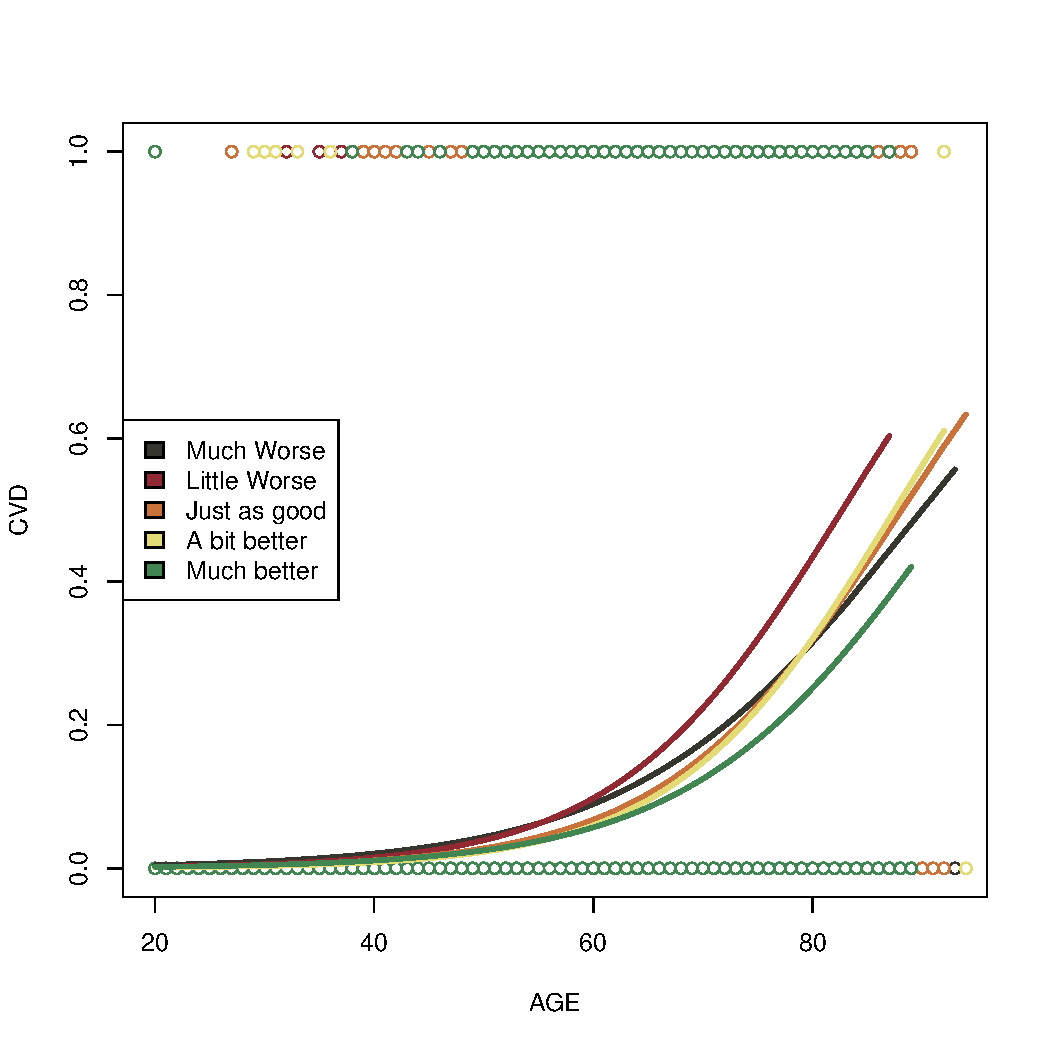
\includegraphics[width=\maxwidth]{figure/RLS_Fitness_Plot-1} 
\end{knitrout}
    
    Attraverso il grafico notiamo che la categoria Fitness:Much better è quella meno
    soggetta rispetto a tutte le altre. Viceversa la categoria Fitness:Little Worse 
    ha più probabilità di incorrere in un problema cardiovascolare. \par
    
    Chi è della categoria Fitness:Much Worse ha meno probabilità rispetto alla          categoria Fitness:Little Worse evidenziando come un problema cardiovascolare
    non è associato perforza a una pessima condizione di salute. \par
    
    In conclusione, per il solo modello di regressione logistica semplice,
    consideriamo la variabile ordinale Fitness come significativa.\par
    
    Nei successivi capitoli considereremo unicamente la variabile ordinale 
    Fitness.
    
  \clearpage

  \subsection{PA}
\begin{knitrout}
\definecolor{shadecolor}{rgb}{0.969, 0.969, 0.969}\color{fgcolor}\begin{kframe}
\begin{alltt}
\hlcom{#PA}
\hlstd{fit.pa} \hlkwb{<-} \hlkwd{glm}\hlstd{(nmc}\hlopt{$}\hlstd{cvd} \hlopt{~} \hlstd{nmc}\hlopt{$}\hlstd{pa,} \hlkwc{family}\hlstd{=binomial)}
\hlkwd{summary}\hlstd{(fit.pa)}
\end{alltt}
\begin{verbatim}
## 
## Call:
## glm(formula = nmc$cvd ~ nmc$pa, family = binomial)
## 
## Deviance Residuals: 
##     Min       1Q   Median       3Q      Max  
## -0.3242  -0.3242  -0.3242  -0.3242   2.4754  
## 
## Coefficients:
##             Estimate Std. Error  z value Pr(>|z|)    
## (Intercept) -2.91978    0.02581 -113.126   <2e-16 ***
## nmc$pa      -0.09610    0.09974   -0.963    0.335    
## ---
## Signif. codes:  0 '***' 0.001 '**' 0.01 '*' 0.05 '.' 0.1 ' ' 1
## 
## (Dispersion parameter for binomial family taken to be 1)
## 
##     Null deviance: 13400  on 33326  degrees of freedom
## Residual deviance: 13399  on 33325  degrees of freedom
## AIC: 13403
## 
## Number of Fisher Scoring iterations: 5
\end{verbatim}
\end{kframe}
\end{knitrout}
    
    Secondo la valutazione del \emph{p-value} la variabile PA, nonostante 
    influisca negativamente per la CVD, non supera il $5\%$ di significatività, 
    risultando non significativa.
    
  \subsection{Smoke}  
\begin{knitrout}
\definecolor{shadecolor}{rgb}{0.969, 0.969, 0.969}\color{fgcolor}\begin{kframe}
\begin{alltt}
\hlcom{#Smoke}
\hlstd{fit.smoke} \hlkwb{<-} \hlkwd{glm}\hlstd{(nmc}\hlopt{$}\hlstd{cvd} \hlopt{~} \hlstd{nmc}\hlopt{$}\hlstd{smoke,} \hlkwc{family}\hlstd{=binomial)}
\hlkwd{summary}\hlstd{(fit.smoke)}
\end{alltt}
\begin{verbatim}
## 
## Call:
## glm(formula = nmc$cvd ~ nmc$smoke, family = binomial)
## 
## Deviance Residuals: 
##     Min       1Q   Median       3Q      Max  
## -0.3402  -0.3186  -0.3186  -0.3186   2.4946  
## 
## Coefficients:
##                 Estimate Std. Error z value Pr(>|z|)    
## (Intercept)     -3.06590    0.09377 -32.696   <2e-16 ***
## nmc$smokeFormer  0.24571    0.10465   2.348   0.0189 *  
## nmc$smokeNO      0.11061    0.09880   1.119   0.2629    
## ---
## Signif. codes:  0 '***' 0.001 '**' 0.01 '*' 0.05 '.' 0.1 ' ' 1
## 
## (Dispersion parameter for binomial family taken to be 1)
## 
##     Null deviance: 13400  on 33326  degrees of freedom
## Residual deviance: 13392  on 33324  degrees of freedom
## AIC: 13398
## 
## Number of Fisher Scoring iterations: 5
\end{verbatim}
\end{kframe}
\end{knitrout}
  
    \begin{itemize}
      \item Le categorie Smoke:Former e Smoke:NO sembrano influire positivamente
            sull'insorgenza di CVD.
      \item Risulta significativa solo la categoria Smoke:Former con valore stimato:
            Smoke:Former $\sim$ 0.246.
    \end{itemize}
    
    Verifichiamo ora il modello di regressione logistica semplice nel caso della 
    variabile ordinale Smoke.
    
\begin{knitrout}
\definecolor{shadecolor}{rgb}{0.969, 0.969, 0.969}\color{fgcolor}\begin{kframe}
\begin{alltt}
\hlcom{#Smoke: Ordinale}
\hlstd{fit.smoke.ord} \hlkwb{<-} \hlkwd{glm}\hlstd{(nmc}\hlopt{$}\hlstd{cvd} \hlopt{~} \hlstd{smoke.ord,} \hlkwc{family}\hlstd{=binomial)}
\hlkwd{summary}\hlstd{(fit.smoke.ord)}
\end{alltt}
\begin{verbatim}
## 
## Call:
## glm(formula = nmc$cvd ~ smoke.ord, family = binomial)
## 
## Deviance Residuals: 
##     Min       1Q   Median       3Q      Max  
## -0.3281  -0.3249  -0.3218  -0.3218   2.4441  
## 
## Coefficients:
##             Estimate Std. Error z value Pr(>|z|)    
## (Intercept) -2.95522    0.06099 -48.454   <2e-16 ***
## smoke.ord    0.02015    0.03893   0.518    0.605    
## ---
## Signif. codes:  0 '***' 0.001 '**' 0.01 '*' 0.05 '.' 0.1 ' ' 1
## 
## (Dispersion parameter for binomial family taken to be 1)
## 
##     Null deviance: 13400  on 33326  degrees of freedom
## Residual deviance: 13400  on 33325  degrees of freedom
## AIC: 13404
## 
## Number of Fisher Scoring iterations: 5
\end{verbatim}
\end{kframe}
\end{knitrout}
    
    \begin{itemize}
      \item La variabile ordinale Smoke risulta positiva nell'insorgenza di CVD.
      \item Nonostante ciò la variabile Smoke ordinale risulta non significativa
            secondo il \emph{p-value}.
    \end{itemize}
    
    Analizziamo se ci siano delle differenze tra le varie categorie di fumatori
    con l'avanzare dell'età.
    
\begin{knitrout}
\definecolor{shadecolor}{rgb}{0.969, 0.969, 0.969}\color{fgcolor}\begin{kframe}
\begin{alltt}
\hlcom{#Smoke NO}
\hlstd{fit.smoke.no} \hlkwb{<-} \hlkwd{glm}\hlstd{(nmc}\hlopt{$}\hlstd{cvd[nmc}\hlopt{$}\hlstd{smoke}\hlopt{==}\hlstr{"NO"}\hlstd{]} \hlopt{~}
                      \hlstd{nmc}\hlopt{$}\hlstd{age[nmc}\hlopt{$}\hlstd{smoke}\hlopt{==}\hlstr{"NO"}\hlstd{],}
                      \hlkwc{family}\hlstd{=binomial)}
\hlstd{pstima.smoke.no} \hlkwb{<-} \hlstd{fit.smoke.no}\hlopt{$}\hlstd{fitted.values}

\hlcom{#Smoke Former}
\hlstd{fit.smoke.former} \hlkwb{<-} \hlkwd{glm}\hlstd{(nmc}\hlopt{$}\hlstd{cvd[nmc}\hlopt{$}\hlstd{smoke}\hlopt{==}\hlstr{"Former"}\hlstd{]} \hlopt{~}
                          \hlstd{nmc}\hlopt{$}\hlstd{age[nmc}\hlopt{$}\hlstd{smoke}\hlopt{==}\hlstr{"Former"}\hlstd{],}
                          \hlkwc{family}\hlstd{=binomial)}
\hlstd{pstima.smoke.former} \hlkwb{<-} \hlstd{fit.smoke.former}\hlopt{$}\hlstd{fitted.values}

\hlcom{#Smoke Current}
\hlstd{fit.smoke.current} \hlkwb{<-} \hlkwd{glm}\hlstd{(nmc}\hlopt{$}\hlstd{cvd[nmc}\hlopt{$}\hlstd{smoke}\hlopt{==}\hlstr{"Current"}\hlstd{]} \hlopt{~}
                           \hlstd{nmc}\hlopt{$}\hlstd{age[nmc}\hlopt{$}\hlstd{smoke}\hlopt{==}\hlstr{"Current"}\hlstd{],}
                           \hlkwc{family}\hlstd{=binomial)}
\hlstd{pstima.smoke.current} \hlkwb{<-} \hlstd{fit.smoke.current}\hlopt{$}\hlstd{fitted.values}

\hlcom{#Plot}
\hlkwd{plot}\hlstd{(nmc}\hlopt{$}\hlstd{age[nmc}\hlopt{$}\hlstd{smoke}\hlopt{==}\hlstr{"NO"}\hlstd{], nmc}\hlopt{$}\hlstd{cvd[nmc}\hlopt{$}\hlstd{smoke}\hlopt{==}\hlstr{"NO"}\hlstd{],}
     \hlkwc{xlab}\hlstd{=}\hlstr{"Age"}\hlstd{,} \hlkwc{ylab}\hlstd{=}\hlstr{"CVD"}\hlstd{,} \hlkwc{col}\hlstd{=}\hlstr{"green"}\hlstd{)}
\hlkwd{points}\hlstd{(nmc}\hlopt{$}\hlstd{age[nmc}\hlopt{$}\hlstd{smoke}\hlopt{==}\hlstr{"Former"}\hlstd{], nmc}\hlopt{$}\hlstd{cvd[nmc}\hlopt{$}\hlstd{smoke}\hlopt{==}\hlstr{"Former"}\hlstd{],}
       \hlkwc{col}\hlstd{=}\hlstr{"orange"}\hlstd{)}
\hlkwd{points}\hlstd{(nmc}\hlopt{$}\hlstd{age[nmc}\hlopt{$}\hlstd{smoke}\hlopt{==}\hlstr{"Current"}\hlstd{], nmc}\hlopt{$}\hlstd{cvd[nmc}\hlopt{$}\hlstd{smoke}\hlopt{==}\hlstr{"Current"}\hlstd{],}
       \hlkwc{col}\hlstd{=}\hlstr{"red"}\hlstd{)}
\hlkwd{lines}\hlstd{(nmc}\hlopt{$}\hlstd{age[nmc}\hlopt{$}\hlstd{smoke}\hlopt{==}\hlstr{"NO"}\hlstd{], pstima.smoke.no,}
      \hlkwc{col}\hlstd{=}\hlstr{"green"}\hlstd{)}
\hlkwd{lines}\hlstd{(nmc}\hlopt{$}\hlstd{age[nmc}\hlopt{$}\hlstd{smoke}\hlopt{==}\hlstr{"Former"}\hlstd{], pstima.smoke.former,}
      \hlkwc{col}\hlstd{=}\hlstr{"orange"}\hlstd{)}
\hlkwd{lines}\hlstd{(nmc}\hlopt{$}\hlstd{age[nmc}\hlopt{$}\hlstd{smoke}\hlopt{==}\hlstr{"Current"}\hlstd{], pstima.smoke.current,}
      \hlkwc{col}\hlstd{=}\hlstr{"red"}\hlstd{)}
\hlkwd{legend}\hlstd{(}\hlkwc{x}\hlstd{=}\hlstr{"left"}\hlstd{,}
       \hlkwc{legend}\hlstd{=}\hlkwd{c}\hlstd{(}\hlstr{"NO"}\hlstd{,} \hlstr{"Former"}\hlstd{,} \hlstr{"Current"}\hlstd{),}
       \hlkwc{lty}\hlstd{=}\hlkwd{c}\hlstd{(}\hlnum{1}\hlstd{,} \hlnum{1}\hlstd{,} \hlnum{1}\hlstd{),}
       \hlkwc{col}\hlstd{=}\hlkwd{c}\hlstd{(}\hlstr{"green"}\hlstd{,}\hlstr{"orange"}\hlstd{,} \hlstr{"red"}\hlstd{),} \hlkwc{lwd}\hlstd{=}\hlnum{1}\hlstd{)}
\end{alltt}
\end{kframe}
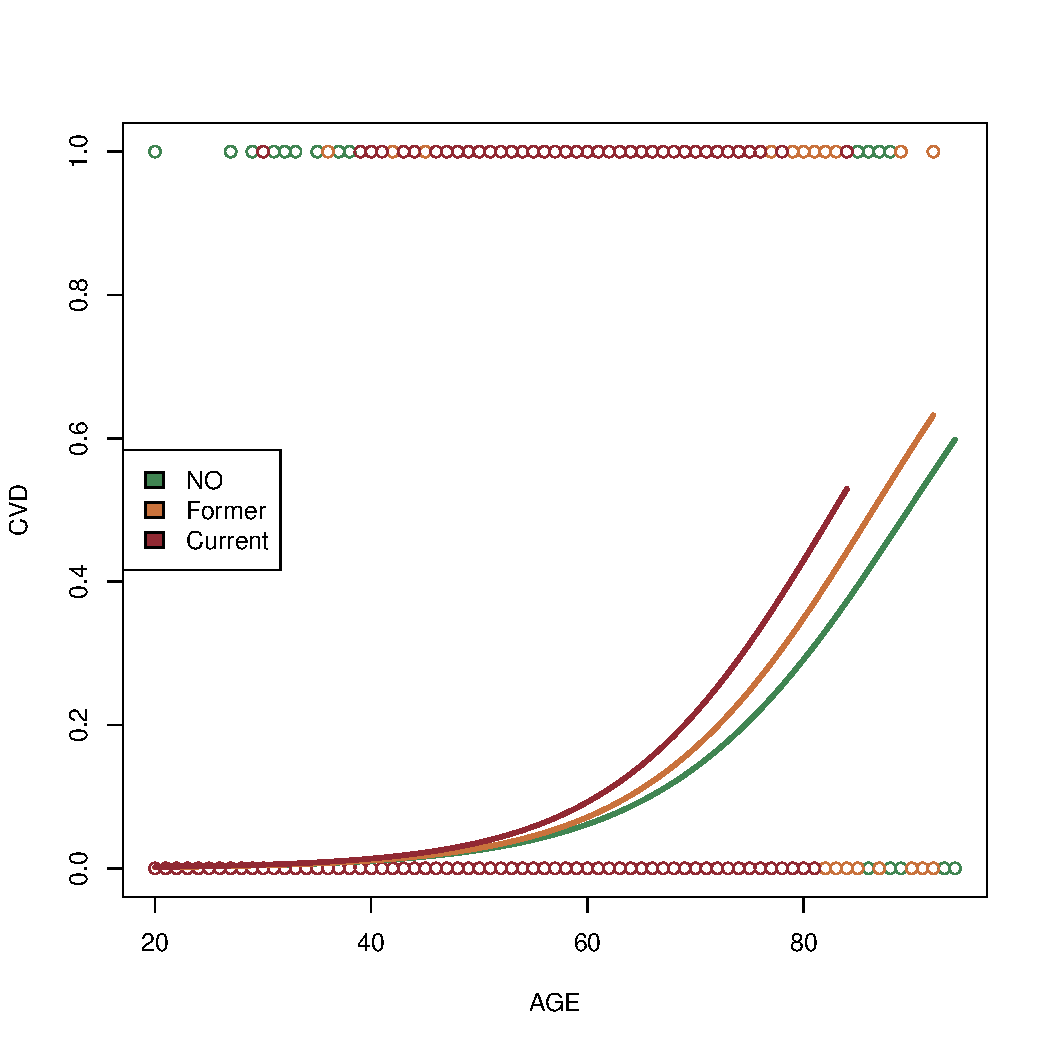
\includegraphics[width=\maxwidth]{figure/RLS_Smoke_Plot-1} 
\end{knitrout}
    
    Possiamo notare come un un fumatore, rispetto alle altre categorie, abbia una       maggiore probabilità di incorrere nella malattia con il passare del tempo.\par
    Viceversa, il non fumatore ha meno probabilità rispetto alle altre categorie di
    incorrere nella malattia. \par
    Nei successivi capitoli considereremo unicamente la variabile categoriale di
    Smoke.
    
  \clearpage  
    
  \subsection{Alchol}
\begin{knitrout}
\definecolor{shadecolor}{rgb}{0.969, 0.969, 0.969}\color{fgcolor}\begin{kframe}
\begin{alltt}
\hlcom{#Alchol}
\hlstd{fit.alc} \hlkwb{<-} \hlkwd{glm}\hlstd{(nmc}\hlopt{$}\hlstd{cvd} \hlopt{~} \hlstd{nmc}\hlopt{$}\hlstd{alc,} \hlkwc{family}\hlstd{=binomial)}
\hlkwd{summary}\hlstd{(fit.alc)}
\end{alltt}
\begin{verbatim}
## 
## Call:
## glm(formula = nmc$cvd ~ nmc$alc, family = binomial)
## 
## Deviance Residuals: 
##     Min       1Q   Median       3Q      Max  
## -0.3241  -0.3235  -0.3230  -0.3230   2.4425  
## 
## Coefficients:
##              Estimate Std. Error z value Pr(>|z|)    
## (Intercept) -2.934597   0.084928  -34.55   <2e-16 ***
## nmc$alc      0.003563   0.035652    0.10     0.92    
## ---
## Signif. codes:  0 '***' 0.001 '**' 0.01 '*' 0.05 '.' 0.1 ' ' 1
## 
## (Dispersion parameter for binomial family taken to be 1)
## 
##     Null deviance: 13400  on 33326  degrees of freedom
## Residual deviance: 13400  on 33325  degrees of freedom
## AIC: 13404
## 
## Number of Fisher Scoring iterations: 5
\end{verbatim}
\end{kframe}
\end{knitrout}
    
    La variabile Alchol, secondo la valutazione del \emph{p-value}, non supera
    il $5\%$ di significatività, risultando non significativa.
  
  \subsection{Commento}
    Nei soli modelli con regressione logistica semplice abbiamo che:
    \begin{itemize}
      \item Le variabili che risultano essere significative secondo la valutazione
            del \emph{p-value} sono: Sex, Age, BMI e Fitness.
      \item Sempre secondo la valutazione del \emph{p-value}, le variabili che 
            invece risultano non significative sono: PA, Smoke e Alchol.
      \item Le variabili Sex:Male, Age e BMI aumentano il rischio di CVD.
      \item La variabile Fitness evidenzia il fatto che chi sta bene è meno
            soggetto alla problematica.
      \item Il fumatore è più soggetto alla malattia rispetto alle altre categorie.
    \end{itemize}
  
\clearpage


\section{Regressioni Logistiche Multiple}
  Consideriamo ora la regressione logistica multipla includendo tutte le variabili
  che sono presenti all'interno del dataset, verificando quali di esse sono più 
  o meno significative per la visualizzazione di un primo modello unico.
  
  \subsection{Modello Completo}
\begin{knitrout}
\definecolor{shadecolor}{rgb}{0.969, 0.969, 0.969}\color{fgcolor}\begin{kframe}
\begin{alltt}
\hlcom{#Regressioni logistiche multiple}
\hlcom{#Modello Completo}
\hlcom{#Variabili: Sex, Age, BMI, Fitness, PA, Smoke, Alchol}
\hlstd{fit.all} \hlkwb{<-} \hlkwd{glm}\hlstd{(nmc}\hlopt{$}\hlstd{cvd} \hlopt{~} \hlstd{nmc}\hlopt{$}\hlstd{sex}\hlopt{+}\hlstd{nmc}\hlopt{$}\hlstd{age}\hlopt{+}\hlstd{nmc}\hlopt{$}\hlstd{bmi}\hlopt{+}\hlstd{nmc}\hlopt{$}\hlstd{fitness}\hlopt{+}
                         \hlstd{nmc}\hlopt{$}\hlstd{pa}\hlopt{+}\hlstd{nmc}\hlopt{$}\hlstd{smoke}\hlopt{+}\hlstd{nmc}\hlopt{$}\hlstd{alc,}
                         \hlkwc{family}\hlstd{=binomial)}
\hlkwd{summary}\hlstd{(fit.all)}
\end{alltt}
\begin{verbatim}
## 
## Call:
## glm(formula = nmc$cvd ~ nmc$sex + nmc$age + nmc$bmi + nmc$fitness + 
##     nmc$pa + nmc$smoke + nmc$alc, family = binomial)
## 
## Deviance Residuals: 
##     Min       1Q   Median       3Q      Max  
## -1.5967  -0.3394  -0.1937  -0.0950   3.6484  
## 
## Coefficients:
##                  Estimate Std. Error z value Pr(>|z|)    
## (Intercept)     -7.475667   0.213543 -35.008  < 2e-16 ***
## nmc$sexMale      0.799132   0.054689  14.612  < 2e-16 ***
## nmc$age          0.092680   0.002446  37.896  < 2e-16 ***
## nmc$bmi          0.235120   0.096986   2.424 0.015339 *  
## nmc$fitness     -0.181741   0.031070  -5.849 4.93e-09 ***
## nmc$pa           0.035563   0.108422   0.328 0.742909    
## nmc$smokeFormer -0.332158   0.111102  -2.990 0.002793 ** 
## nmc$smokeNO     -0.374001   0.106486  -3.512 0.000444 ***
## nmc$alc         -0.056404   0.035625  -1.583 0.113368    
## ---
## Signif. codes:  0 '***' 0.001 '**' 0.01 '*' 0.05 '.' 0.1 ' ' 1
## 
## (Dispersion parameter for binomial family taken to be 1)
## 
##     Null deviance: 13400  on 33326  degrees of freedom
## Residual deviance: 10883  on 33318  degrees of freedom
## AIC: 10901
## 
## Number of Fisher Scoring iterations: 7
\end{verbatim}
\end{kframe}
\end{knitrout}
    
    Per il modello che include tutte le variabili:\\
    Modello: CVD $\sim$ Sex + Age + BMI + Fitness + PA + Smoke + Alchol 
    \begin{itemize}
      \item Risultano essere significative, secondo il \emph{p-value}, le 
            variabili: Sex, Age, BMI, Fitness e Smoke.
      \item Risultano essere non significative, non superando il $5\%$
            di significatività del \emph{p-value}, le variabili: PA e Alchol.
      \item I parametri stimati nella regressione logistica multipla differescono da             quelli presenti nelle regressioni logistiche semplici precedentemente               analizzate.
      \item Gli errori standard non differiscono molto da quelli presenti nei                   modelli con regressione logistica semplice.
      \item La variabile Sex mostra ancora come il sesso Maschile influisca 
            positivamente nella presenza di CVD con valore stimato: 
            Sex:Male $\sim$ 0.788.
      \item Anche le variabili BMI e Smoke mostrano un aumento nelle possibilità 
            di insorgenza di un CVD.
      \item La variabile Fitness aumenta di significatività, rispetto
            al modello di regressione logistica semplice, riducendo la 
            probabilità di CVD con valore stimato: Fitness $\sim$ -0.184.
    \end{itemize}
  
  \subsection{Modello Significativo}
    Dato che nel modello completo sono presenti variabili non significative,
    le andremo ad eliminare gradualmente dalla formula del modello fino ad 
    ottenere un modello con solo variabili significative.\par
    Iniziamo eliminando la variabile non significativa PA.
    
\begin{knitrout}
\definecolor{shadecolor}{rgb}{0.969, 0.969, 0.969}\color{fgcolor}\begin{kframe}
\begin{alltt}
\hlcom{#Modello senza PA}
\hlcom{#Variabili: Sex, Age, BMI, Fitness, Smoke, Alchol}
\hlstd{fit.npa} \hlkwb{<-} \hlkwd{glm}\hlstd{(nmc}\hlopt{$}\hlstd{cvd} \hlopt{~} \hlstd{nmc}\hlopt{$}\hlstd{sex}\hlopt{+}\hlstd{nmc}\hlopt{$}\hlstd{age}\hlopt{+}\hlstd{nmc}\hlopt{$}\hlstd{bmi}\hlopt{+}\hlstd{nmc}\hlopt{$}\hlstd{fitness}\hlopt{+}
                         \hlstd{nmc}\hlopt{$}\hlstd{smoke}\hlopt{+}\hlstd{nmc}\hlopt{$}\hlstd{alc,}
                         \hlkwc{family}\hlstd{=binomial)}
\hlkwd{summary}\hlstd{(fit.npa)}
\end{alltt}
\begin{verbatim}
## 
## Call:
## glm(formula = nmc$cvd ~ nmc$sex + nmc$age + nmc$bmi + nmc$fitness + 
##     nmc$smoke + nmc$alc, family = binomial)
## 
## Deviance Residuals: 
##     Min       1Q   Median       3Q      Max  
## -1.5978  -0.3371  -0.1941  -0.0950   3.6471  
## 
## Coefficients:
##                  Estimate Std. Error z value Pr(>|z|)    
## (Intercept)     -7.462934   0.209921 -35.551  < 2e-16 ***
## nmc$sexMale      0.799887   0.054643  14.638  < 2e-16 ***
## nmc$age          0.092640   0.002442  37.930  < 2e-16 ***
## nmc$bmi          0.235857   0.096958   2.433 0.014992 *  
## nmc$fitness     -0.183877   0.030378  -6.053 1.42e-09 ***
## nmc$smokeFormer -0.332592   0.111097  -2.994 0.002756 ** 
## nmc$smokeNO     -0.374525   0.106476  -3.517 0.000436 ***
## nmc$alc         -0.056553   0.035625  -1.587 0.112413    
## ---
## Signif. codes:  0 '***' 0.001 '**' 0.01 '*' 0.05 '.' 0.1 ' ' 1
## 
## (Dispersion parameter for binomial family taken to be 1)
## 
##     Null deviance: 13400  on 33326  degrees of freedom
## Residual deviance: 10883  on 33319  degrees of freedom
## AIC: 10899
## 
## Number of Fisher Scoring iterations: 7
\end{verbatim}
\end{kframe}
\end{knitrout}
    
    Tutte le varibili che erano significative nel modello completo risultano 
    ancora significative. \par
    Eliminiamo la variabile Alchol, che risulta ancora non significativa,
    all'interno della formula.
    
\begin{knitrout}
\definecolor{shadecolor}{rgb}{0.969, 0.969, 0.969}\color{fgcolor}\begin{kframe}
\begin{alltt}
\hlcom{#Modello significativo}
\hlcom{#Variabili: Sex, Age, BMI, Fitness, Smoke }
\hlstd{fit} \hlkwb{<-} \hlkwd{glm}\hlstd{(nmc}\hlopt{$}\hlstd{cvd} \hlopt{~} \hlstd{nmc}\hlopt{$}\hlstd{sex}\hlopt{+}\hlstd{nmc}\hlopt{$}\hlstd{age}\hlopt{+}\hlstd{nmc}\hlopt{$}\hlstd{bmi}\hlopt{+}\hlstd{nmc}\hlopt{$}\hlstd{fitness}\hlopt{+}
                     \hlstd{nmc}\hlopt{$}\hlstd{smoke,} \hlkwc{family}\hlstd{=binomial)}
\hlkwd{summary}\hlstd{(fit)}
\end{alltt}
\begin{verbatim}
## 
## Call:
## glm(formula = nmc$cvd ~ nmc$sex + nmc$age + nmc$bmi + nmc$fitness + 
##     nmc$smoke, family = binomial)
## 
## Deviance Residuals: 
##     Min       1Q   Median       3Q      Max  
## -1.6215  -0.3381  -0.1935  -0.0943   3.6515  
## 
## Coefficients:
##                  Estimate Std. Error z value Pr(>|z|)    
## (Intercept)     -7.614728   0.187445 -40.624  < 2e-16 ***
## nmc$sexMale      0.786417   0.053959  14.574  < 2e-16 ***
## nmc$age          0.092988   0.002437  38.159  < 2e-16 ***
## nmc$bmi          0.240200   0.096914   2.478 0.013194 *  
## nmc$fitness     -0.186214   0.030344  -6.137 8.42e-10 ***
## nmc$smokeFormer -0.331879   0.111118  -2.987 0.002820 ** 
## nmc$smokeNO     -0.351977   0.105515  -3.336 0.000851 ***
## ---
## Signif. codes:  0 '***' 0.001 '**' 0.01 '*' 0.05 '.' 0.1 ' ' 1
## 
## (Dispersion parameter for binomial family taken to be 1)
## 
##     Null deviance: 13400  on 33326  degrees of freedom
## Residual deviance: 10886  on 33320  degrees of freedom
## AIC: 10900
## 
## Number of Fisher Scoring iterations: 7
\end{verbatim}
\end{kframe}
\end{knitrout}
    
    Il modello risultate è: \\
    Modello: CVD $\sim$ Sex + Age + BMI + Fitness + Smoke
    \begin{itemize}
      \item Le variabili risultato essere tutte significative secondo il 
            $\emph{p-value}$.
      \item I parametri stimati e gli errori standard non differiscono molto dal 
            modello completo.
    \end{itemize}
    
    Il modello con solo variabili significative sembra mostrare un buon 
    adattamento.\par
    Visualizziamo il grafico dell'andamento del modello stimato.
    
\begin{knitrout}
\definecolor{shadecolor}{rgb}{0.969, 0.969, 0.969}\color{fgcolor}\begin{kframe}
\begin{alltt}
\hlstd{pstima} \hlkwb{<-} \hlstd{fit}\hlopt{$}\hlstd{fitted.values}

\hlcom{#Plot}
\hlkwd{plot}\hlstd{(nmc}\hlopt{$}\hlstd{age, nmc}\hlopt{$}\hlstd{cvd,} \hlkwc{xlab}\hlstd{=}\hlstr{"Age"}\hlstd{,} \hlkwc{ylab}\hlstd{=}\hlstr{"CVD"}\hlstd{)}
\hlkwd{points}\hlstd{(}\hlkwd{sort}\hlstd{(nmc}\hlopt{$}\hlstd{age), pstima[}\hlkwd{order}\hlstd{(nmc}\hlopt{$}\hlstd{age)],} \hlkwc{col}\hlstd{=}\hlstr{"blue"}\hlstd{)}
\end{alltt}
\end{kframe}
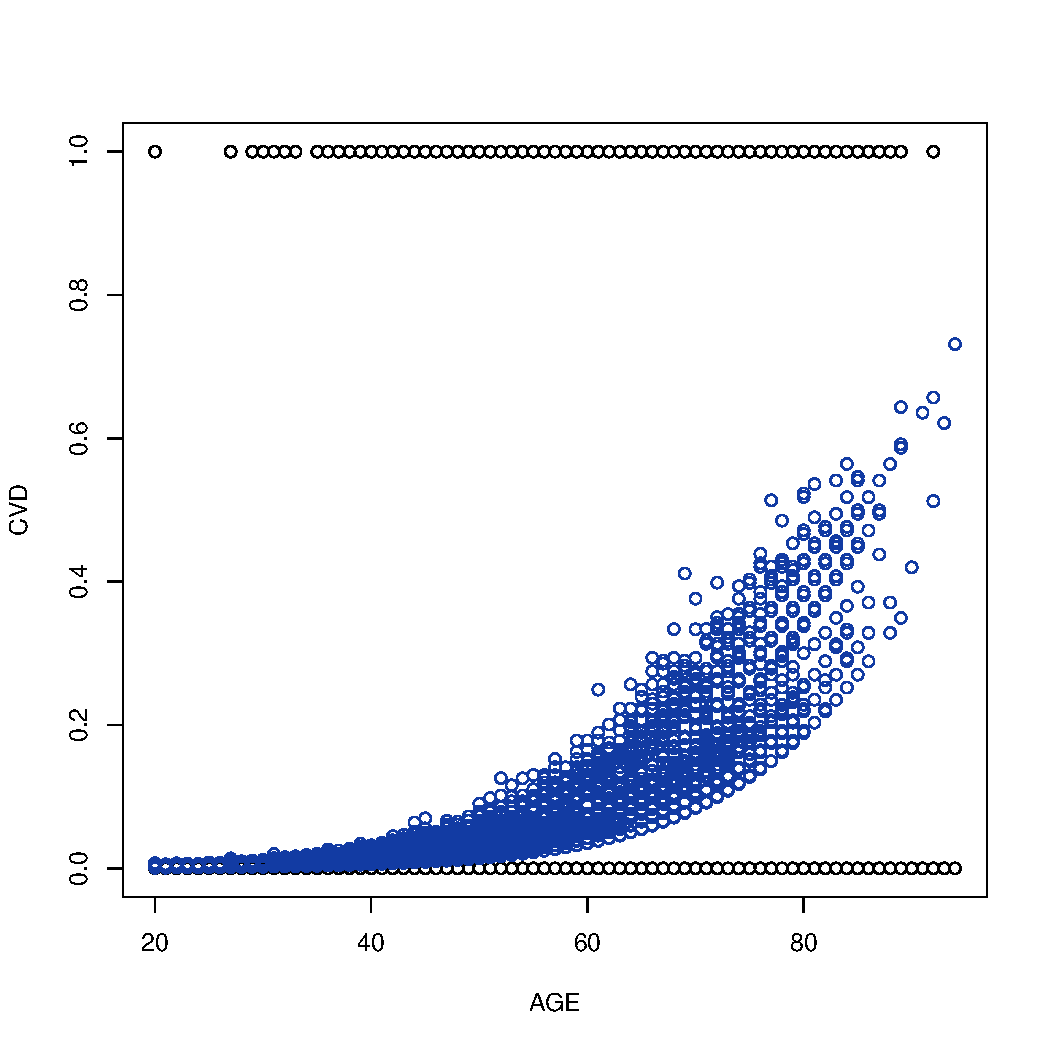
\includegraphics[width=\maxwidth]{figure/RLM_Plot_ModelloSignificativo-1} 
\end{knitrout}
  
  \subsection{Commento}
    \begin{itemize}
      \item Il modello risulta essere: \\
            Modello: CVD$\sim$ Sex + Age + BMI + Fitness + Smoke
      \item Come visto nelle regressioni logistiche semplici, le variabili
            sexMale, Age e BMI continuano ad influenzare positivamente la 
            comparsa di problemi cardiovascolari.
      \item Al contrario, le variabili significative Fitness e Smoke (per la 
            categoria "Former" e la categoria "NO") riducono la possibilità di 
            avere un CVD.
      \item Di conseguenza la categoria Smoke:Current ha una probabilità 
            maggiore nell'insorgenza di CVD.
    \end{itemize}
  
  \subsection{Dati di esempio}
    Effettuiamo una valutazione della probabilità su degli individui casuali 
    in base ai modelli precedentemente analizzati. \par
    Visualizziamo i coefficienti del modello completo e quello significativo.
    
\begin{knitrout}
\definecolor{shadecolor}{rgb}{0.969, 0.969, 0.969}\color{fgcolor}\begin{kframe}
\begin{alltt}
\hlcom{#Coefficienti Modello Completo}
\hlkwd{coef}\hlstd{(fit.all)}
\end{alltt}
\begin{verbatim}
##     (Intercept)     nmc$sexMale         nmc$age         nmc$bmi     nmc$fitness 
##     -7.47566727      0.79913169      0.09267966      0.23512007     -0.18174054 
##          nmc$pa nmc$smokeFormer     nmc$smokeNO         nmc$alc 
##      0.03556271     -0.33215760     -0.37400050     -0.05640352
\end{verbatim}
\end{kframe}
\end{knitrout}
    
\begin{knitrout}
\definecolor{shadecolor}{rgb}{0.969, 0.969, 0.969}\color{fgcolor}\begin{kframe}
\begin{alltt}
\hlcom{#Coefficienti Modello Significativo}
\hlkwd{coef}\hlstd{(fit)}
\end{alltt}
\begin{verbatim}
##     (Intercept)     nmc$sexMale         nmc$age         nmc$bmi     nmc$fitness 
##     -7.61472806      0.78641659      0.09298766      0.24020007     -0.18621360 
## nmc$smokeFormer     nmc$smokeNO 
##     -0.33187854     -0.35197684
\end{verbatim}
\end{kframe}
\end{knitrout}
    
    Verifichiamo la probabilità di avere un CVD per un Uomo (Sex 1) di 45 anni 
    fumatore, con BMI pari a 32 (BMI dicotomizzato a 1), che non fa consumo di 
    alchol (Alchol 1), in ottima salute (Fitness 5) e PA=1.
    
\begin{knitrout}
\definecolor{shadecolor}{rgb}{0.969, 0.969, 0.969}\color{fgcolor}\begin{kframe}
\begin{alltt}
\hlcom{#Stima per il Modello Completo}
\hlcom{#Dato}
\hlcom{#Intercetta: 1, Sex: 1, Age: 45, BMI: 1, Fitness: 5, }
\hlcom{#PA: 1, Smoke:Former: 0, Smoke:NO: 0, Alchol: 1 }
\hlstd{man45.all} \hlkwb{<-} \hlkwd{c}\hlstd{(}\hlnum{1}\hlstd{,} \hlnum{1}\hlstd{,} \hlnum{45}\hlstd{,} \hlnum{1}\hlstd{,} \hlnum{5}\hlstd{,} \hlnum{1}\hlstd{,} \hlnum{0}\hlstd{,} \hlnum{0}\hlstd{,} \hlnum{1}\hlstd{)}
\hlstd{stima.man45.all} \hlkwb{<-} \hlkwd{exp}\hlstd{(}\hlkwd{coef}\hlstd{(fit.all)}\hlopt\hlstd{man45.all)}\hlopt{/}
                       \hlstd{(}\hlnum{1}\hlopt{+}\hlkwd{exp}\hlstd{(}\hlkwd{coef}\hlstd{(fit.all)}\hlopt\hlstd{man45.all))}
\hlstd{stima.man45.all}
\end{alltt}
\begin{verbatim}
##            [,1]
## [1,] 0.03915164
\end{verbatim}
\end{kframe}
\end{knitrout}
    
\begin{knitrout}
\definecolor{shadecolor}{rgb}{0.969, 0.969, 0.969}\color{fgcolor}\begin{kframe}
\begin{alltt}
\hlcom{#Stima per il Modello Significativo}
\hlcom{#Dato}
\hlcom{#Intercetta: 1, Sex: 1, Age: 45, BMI: 1, Fitness: 5, }
\hlcom{#Smoke:Former: 0, Smoke:NO: 0}
\hlstd{man45} \hlkwb{<-} \hlkwd{c}\hlstd{(}\hlnum{1}\hlstd{,} \hlnum{1}\hlstd{,} \hlnum{45}\hlstd{,} \hlnum{1}\hlstd{,} \hlnum{5}\hlstd{,} \hlnum{0}\hlstd{,} \hlnum{0}\hlstd{)}
\hlstd{stima.man45} \hlkwb{<-} \hlkwd{exp}\hlstd{(}\hlkwd{coef}\hlstd{(fit)}\hlopt\hlstd{man45)}\hlopt{/}\hlstd{(}\hlnum{1}\hlopt{+}\hlkwd{exp}\hlstd{(}\hlkwd{coef}\hlstd{(fit)}\hlopt\hlstd{man45))}
\hlstd{stima.man45}
\end{alltt}
\begin{verbatim}
##            [,1]
## [1,] 0.03439862
\end{verbatim}
\end{kframe}
\end{knitrout}
    
    Risulta che:
    \begin{itemize}
      \item per il Modello Completo: $\hat{\pi}$ = 0.0391
      \item per il Modello Significativo: $\hat{\pi}$ = 0.0343
    \end{itemize}
    
    Verifichiamo adesso la probabilità di avere un CVD per una Donna (Sex 0) di 
    60 anni ex fumatrice, con BMI pari a 35 (BMI dicotomizzato 1), che beve 
    alchol nella media (Alchol 4), in buona salute (Fitness 4), e PA = 1.
    
\begin{knitrout}
\definecolor{shadecolor}{rgb}{0.969, 0.969, 0.969}\color{fgcolor}\begin{kframe}
\begin{alltt}
\hlcom{#Stima per il Modello Completo}
\hlcom{#Dato}
\hlcom{#Intercetta: 1, Sex: 0, Age: 60, BMI: 1, Fitness: 4, }
\hlcom{#PA: 1, Smoke:Former: 1, Smoke:NO: 0, Alchol: 4 }
\hlstd{woman60.all} \hlkwb{<-} \hlkwd{c}\hlstd{(}\hlnum{1}\hlstd{,} \hlnum{0}\hlstd{,} \hlnum{60}\hlstd{,} \hlnum{1}\hlstd{,} \hlnum{4}\hlstd{,} \hlnum{1}\hlstd{,} \hlnum{1}\hlstd{,} \hlnum{0}\hlstd{,} \hlnum{4}\hlstd{)}
\hlstd{stima.woman60.all} \hlkwb{<-} \hlkwd{exp}\hlstd{(}\hlkwd{coef}\hlstd{(fit.all)}\hlopt\hlstd{woman60.all)}\hlopt{/}
                       \hlstd{(}\hlnum{1}\hlopt{+}\hlkwd{exp}\hlstd{(}\hlkwd{coef}\hlstd{(fit.all)}\hlopt\hlstd{woman60.all))}
\hlstd{stima.woman60.all}
\end{alltt}
\begin{verbatim}
##            [,1]
## [1,] 0.05074142
\end{verbatim}
\end{kframe}
\end{knitrout}
    
\begin{knitrout}
\definecolor{shadecolor}{rgb}{0.969, 0.969, 0.969}\color{fgcolor}\begin{kframe}
\begin{alltt}
\hlcom{#Stima per il Modello Significativo}
\hlcom{#Intercetta: 1, Sex: 0, Age: 60, BMI: 1, Fitness: 4, }
\hlcom{#Smoke:Former: 1, Smoke:NO: 0}
\hlstd{woman60} \hlkwb{<-} \hlkwd{c}\hlstd{(}\hlnum{1}\hlstd{,} \hlnum{0}\hlstd{,} \hlnum{60}\hlstd{,} \hlnum{1}\hlstd{,} \hlnum{4}\hlstd{,} \hlnum{1}\hlstd{,} \hlnum{0}\hlstd{)}
\hlstd{stima.woman60} \hlkwb{<-} \hlkwd{exp}\hlstd{(}\hlkwd{coef}\hlstd{(fit)}\hlopt\hlstd{woman60)}\hlopt{/}\hlstd{(}\hlnum{1}\hlopt{+}\hlkwd{exp}\hlstd{(}\hlkwd{coef}\hlstd{(fit)}\hlopt\hlstd{woman60))}
\hlstd{stima.woman60}
\end{alltt}
\begin{verbatim}
##            [,1]
## [1,] 0.05355512
\end{verbatim}
\end{kframe}
\end{knitrout}
    
    Risulta che:
    \begin{itemize}
      \item Modello Completo: $\hat{\pi}$ = 0.0507
      \item Modello Significativo: $\hat{\pi}$ = 0.0535
    \end{itemize}
    
    In conclusione possiamo vedere come la probabilità del modello completo e
    del modello con solo variabili significative si mostrino particolarmente 
    simili.

\clearpage    


\section{Considerazioni sul Modello}
  In questo capitolo confronteremo il comportamento del modello su una specifica      categoria di invidividui.

  \subsection{Maschio e Femmina} 
    Nei precedenti capitoli, durante l'analisi delle singole variabili e dei vari 
    modelli, abbiamo notato come ci siano stati sempre diverse probabilità 
    tra il sesso maschile e il sesso femmile.\par
    Valutiamo ancora all'interno di un grafico se questa nostra ipotesi si 
    verifica in un modello più complesso di quello marginale.
      
\begin{knitrout}
\definecolor{shadecolor}{rgb}{0.969, 0.969, 0.969}\color{fgcolor}\begin{kframe}
\begin{alltt}
\hlcom{#Modello Sesso Maschile}
\hlcom{#Sex: Male}
\hlstd{fit.male} \hlkwb{<-} \hlkwd{glm}\hlstd{(nmc}\hlopt{$}\hlstd{cvd[nmc}\hlopt{$}\hlstd{sex}\hlopt{==}\hlstr{"Male"}\hlstd{]} \hlopt{~}
                  \hlstd{nmc}\hlopt{$}\hlstd{age[nmc}\hlopt{$}\hlstd{sex}\hlopt{==}\hlstr{"Male"}\hlstd{]}\hlopt{+}
                  \hlstd{nmc}\hlopt{$}\hlstd{bmi[nmc}\hlopt{$}\hlstd{sex}\hlopt{==}\hlstr{"Male"}\hlstd{]}\hlopt{+}
                  \hlstd{nmc}\hlopt{$}\hlstd{fitness[nmc}\hlopt{$}\hlstd{sex}\hlopt{==}\hlstr{"Male"}\hlstd{]}\hlopt{+}
                  \hlstd{nmc}\hlopt{$}\hlstd{smoke[nmc}\hlopt{$}\hlstd{sex}\hlopt{==}\hlstr{"Male"}\hlstd{],}
                  \hlkwc{family}\hlstd{=binomial)}
\hlkwd{summary}\hlstd{(fit.male)}
\end{alltt}
\begin{verbatim}
## 
## Call:
## glm(formula = nmc$cvd[nmc$sex == "Male"] ~ nmc$age[nmc$sex == 
##     "Male"] + nmc$bmi[nmc$sex == "Male"] + nmc$fitness[nmc$sex == 
##     "Male"] + nmc$smoke[nmc$sex == "Male"], family = binomial)
## 
## Deviance Residuals: 
##     Min       1Q   Median       3Q      Max  
## -1.5009  -0.4634  -0.2744  -0.1136   3.4503  
## 
## Coefficients:
##                                     Estimate Std. Error z value Pr(>|z|)    
## (Intercept)                        -6.310134   0.257771 -24.480  < 2e-16 ***
## nmc$age[nmc$sex == "Male"]          0.086098   0.003316  25.968  < 2e-16 ***
## nmc$bmi[nmc$sex == "Male"]          0.135192   0.157317   0.859 0.390142    
## nmc$fitness[nmc$sex == "Male"]     -0.156521   0.042188  -3.710 0.000207 ***
## nmc$smoke[nmc$sex == "Male"]Former -0.472766   0.146244  -3.233 0.001226 ** 
## nmc$smoke[nmc$sex == "Male"]NO     -0.579023   0.142624  -4.060 4.91e-05 ***
## ---
## Signif. codes:  0 '***' 0.001 '**' 0.01 '*' 0.05 '.' 0.1 ' ' 1
## 
## (Dispersion parameter for binomial family taken to be 1)
## 
##     Null deviance: 6344.1  on 11129  degrees of freedom
## Residual deviance: 5297.3  on 11124  degrees of freedom
## AIC: 5309.3
## 
## Number of Fisher Scoring iterations: 6
\end{verbatim}
\begin{alltt}
\hlstd{pstima.male} \hlkwb{<-} \hlstd{fit.male}\hlopt{$}\hlstd{fitted.values}
\end{alltt}
\end{kframe}
\end{knitrout}
    
\begin{knitrout}
\definecolor{shadecolor}{rgb}{0.969, 0.969, 0.969}\color{fgcolor}\begin{kframe}
\begin{alltt}
\hlcom{#Modello Sesso Femminile}
\hlcom{#Sex: Female}
\hlstd{fit.female} \hlkwb{<-} \hlkwd{glm}\hlstd{(nmc}\hlopt{$}\hlstd{cvd[nmc}\hlopt{$}\hlstd{sex}\hlopt{==}\hlstr{"Female"}\hlstd{]} \hlopt{~}
                    \hlstd{nmc}\hlopt{$}\hlstd{age[nmc}\hlopt{$}\hlstd{sex}\hlopt{==}\hlstr{"Female"}\hlstd{]}\hlopt{+}
                    \hlstd{nmc}\hlopt{$}\hlstd{bmi[nmc}\hlopt{$}\hlstd{sex}\hlopt{==}\hlstr{"Female"}\hlstd{]}\hlopt{+}
                    \hlstd{nmc}\hlopt{$}\hlstd{fitness[nmc}\hlopt{$}\hlstd{sex}\hlopt{==}\hlstr{"Female"}\hlstd{]}\hlopt{+}
                    \hlstd{nmc}\hlopt{$}\hlstd{smoke[nmc}\hlopt{$}\hlstd{sex}\hlopt{==}\hlstr{"Female"}\hlstd{],}
                    \hlkwc{family}\hlstd{=binomial)}
\hlkwd{summary}\hlstd{(fit.female)}
\end{alltt}
\begin{verbatim}
## 
## Call:
## glm(formula = nmc$cvd[nmc$sex == "Female"] ~ nmc$age[nmc$sex == 
##     "Female"] + nmc$bmi[nmc$sex == "Female"] + nmc$fitness[nmc$sex == 
##     "Female"] + nmc$smoke[nmc$sex == "Female"], family = binomial)
## 
## Deviance Residuals: 
##     Min       1Q   Median       3Q      Max  
## -1.5166  -0.2829  -0.1632  -0.0847   3.7175  
## 
## Coefficients:
##                                       Estimate Std. Error z value Pr(>|z|)    
## (Intercept)                          -8.132620   0.277110 -29.348  < 2e-16 ***
## nmc$age[nmc$sex == "Female"]          0.099409   0.003598  27.630  < 2e-16 ***
## nmc$bmi[nmc$sex == "Female"]          0.284497   0.123459   2.304   0.0212 *  
## nmc$fitness[nmc$sex == "Female"]     -0.210839   0.043547  -4.842 1.29e-06 ***
## nmc$smoke[nmc$sex == "Female"]Former -0.182839   0.174076  -1.050   0.2936    
## nmc$smoke[nmc$sex == "Female"]NO     -0.132124   0.160494  -0.823   0.4104    
## ---
## Signif. codes:  0 '***' 0.001 '**' 0.01 '*' 0.05 '.' 0.1 ' ' 1
## 
## (Dispersion parameter for binomial family taken to be 1)
## 
##     Null deviance: 6729.3  on 22196  degrees of freedom
## Residual deviance: 5573.1  on 22191  degrees of freedom
## AIC: 5585.1
## 
## Number of Fisher Scoring iterations: 7
\end{verbatim}
\begin{alltt}
\hlstd{pstima.female} \hlkwb{<-} \hlstd{fit.female}\hlopt{$}\hlstd{fitted.values}
\end{alltt}
\end{kframe}
\end{knitrout}
    
\begin{knitrout}
\definecolor{shadecolor}{rgb}{0.969, 0.969, 0.969}\color{fgcolor}\begin{kframe}
\begin{alltt}
\hlcom{#Plot}
\hlkwd{plot}\hlstd{(nmc}\hlopt{$}\hlstd{age[nmc}\hlopt{$}\hlstd{sex}\hlopt{==}\hlstr{"Male"}\hlstd{], nmc}\hlopt{$}\hlstd{cvd[nmc}\hlopt{$}\hlstd{sex}\hlopt{==}\hlstr{"Male"}\hlstd{],}
     \hlkwc{xlab}\hlstd{=}\hlstr{"Age"}\hlstd{,} \hlkwc{ylab}\hlstd{=}\hlstr{"CVD"}\hlstd{,} \hlkwc{col}\hlstd{=}\hlstr{"blue"}\hlstd{)}
\hlkwd{points}\hlstd{(nmc}\hlopt{$}\hlstd{age[nmc}\hlopt{$}\hlstd{sex}\hlopt{==}\hlstr{"Female"}\hlstd{], nmc}\hlopt{$}\hlstd{cvd[nmc}\hlopt{$}\hlstd{sex}\hlopt{==}\hlstr{"Female"}\hlstd{],}
       \hlkwc{col}\hlstd{=}\hlstr{"red"}\hlstd{)}
\hlkwd{points}\hlstd{(}\hlkwd{sort}\hlstd{(nmc}\hlopt{$}\hlstd{age[nmc}\hlopt{$}\hlstd{sex}\hlopt{==}\hlstr{"Male"}\hlstd{]),}
      \hlstd{pstima.male[}\hlkwd{order}\hlstd{(nmc}\hlopt{$}\hlstd{age[nmc}\hlopt{$}\hlstd{sex}\hlopt{==}\hlstr{"Male"}\hlstd{])],}
      \hlkwc{col}\hlstd{=}\hlstr{"blue"}\hlstd{)}
\hlkwd{points}\hlstd{(}\hlkwd{sort}\hlstd{(nmc}\hlopt{$}\hlstd{age[nmc}\hlopt{$}\hlstd{sex}\hlopt{==}\hlstr{"Female"}\hlstd{]),}
      \hlstd{pstima.female[}\hlkwd{order}\hlstd{(nmc}\hlopt{$}\hlstd{age[nmc}\hlopt{$}\hlstd{sex}\hlopt{==}\hlstr{"Female"}\hlstd{])],}
      \hlkwc{col}\hlstd{=}\hlstr{"red"}\hlstd{)}
\hlkwd{legend}\hlstd{(}\hlkwc{x}\hlstd{=}\hlstr{"left"}\hlstd{,} \hlkwc{legend}\hlstd{=}\hlkwd{c}\hlstd{(}\hlstr{"Male"}\hlstd{,} \hlstr{"Female"}\hlstd{),} \hlkwc{lty}\hlstd{=}\hlkwd{c}\hlstd{(}\hlnum{1}\hlstd{,} \hlnum{1}\hlstd{),}
       \hlkwc{col}\hlstd{=}\hlkwd{c}\hlstd{(}\hlstr{"blue"}\hlstd{,}\hlstr{"red"}\hlstd{),} \hlkwc{lwd}\hlstd{=}\hlnum{1}\hlstd{)}
\end{alltt}
\end{kframe}
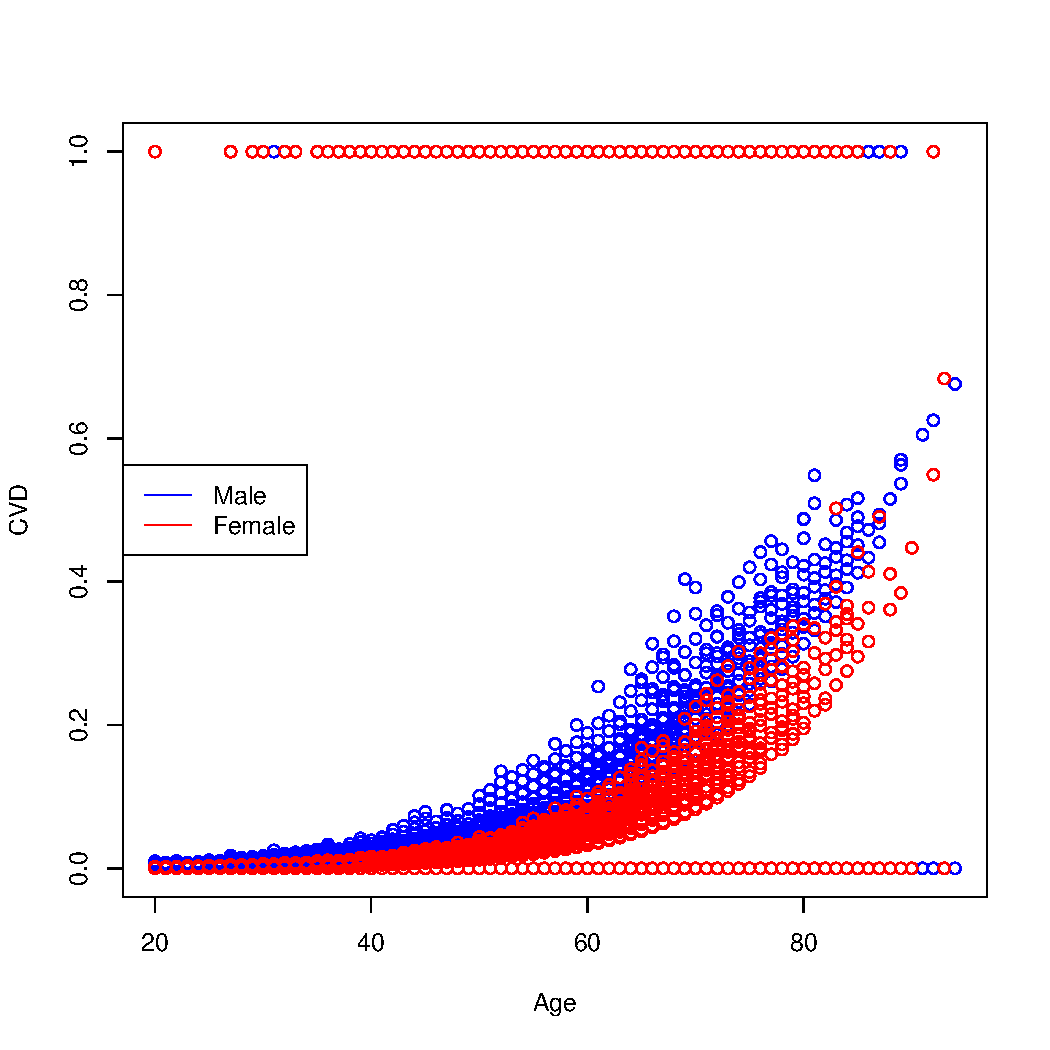
\includegraphics[width=\maxwidth]{figure/Plot_Analisi_ModelloSex-1} 
\end{knitrout}
    
    Statisticamente il sesso maschile rimane il soggetto che ha più rischi di 
    CVD rispetto al genere femminile, anche nel modello più complesso.
  
  \subsection{Attività Fisica}
    Dato che la variabile PA nelle valutazione dei modelli è sempre stata 
    scartata, verifichiamo se all'interno del nostro modello possono esserci 
    delle differenze tra le due categorie di PA per il calcolo del CVD.
    
\begin{knitrout}
\definecolor{shadecolor}{rgb}{0.969, 0.969, 0.969}\color{fgcolor}\begin{kframe}
\begin{alltt}
\hlcom{#Modello PA 0}
\hlstd{fit.pa.0} \hlkwb{<-} \hlkwd{glm}\hlstd{(nmc}\hlopt{$}\hlstd{cvd[nmc}\hlopt{$}\hlstd{pa}\hlopt{==}\hlnum{0}\hlstd{]} \hlopt{~} \hlstd{nmc}\hlopt{$}\hlstd{sex[nmc}\hlopt{$}\hlstd{pa}\hlopt{==}\hlnum{0}\hlstd{]} \hlopt{+}
                  \hlstd{nmc}\hlopt{$}\hlstd{age[nmc}\hlopt{$}\hlstd{pa}\hlopt{==}\hlnum{0}\hlstd{]} \hlopt{+} \hlstd{nmc}\hlopt{$}\hlstd{bmi[nmc}\hlopt{$}\hlstd{pa}\hlopt{==}\hlnum{0}\hlstd{]} \hlopt{+}
                  \hlstd{nmc}\hlopt{$}\hlstd{fitness[nmc}\hlopt{$}\hlstd{pa}\hlopt{==}\hlnum{0}\hlstd{]} \hlopt{+} \hlstd{nmc}\hlopt{$}\hlstd{smoke[nmc}\hlopt{$}\hlstd{pa}\hlopt{==}\hlnum{0}\hlstd{],}
                \hlkwc{family}\hlstd{=binomial)}
\hlkwd{summary}\hlstd{(fit.pa.0)}
\end{alltt}
\begin{verbatim}
## 
## Call:
## glm(formula = nmc$cvd[nmc$pa == 0] ~ nmc$sex[nmc$pa == 0] + nmc$age[nmc$pa == 
##     0] + nmc$bmi[nmc$pa == 0] + nmc$fitness[nmc$pa == 0] + nmc$smoke[nmc$pa == 
##     0], family = binomial)
## 
## Deviance Residuals: 
##     Min       1Q   Median       3Q      Max  
## -1.6202  -0.3396  -0.1936  -0.0931   3.6511  
## 
## Coefficients:
##                               Estimate Std. Error z value Pr(>|z|)    
## (Intercept)                  -7.644393   0.199721 -38.275  < 2e-16 ***
## nmc$sex[nmc$pa == 0]Male      0.782201   0.055911  13.990  < 2e-16 ***
## nmc$age[nmc$pa == 0]          0.092985   0.002545  36.533  < 2e-16 ***
## nmc$bmi[nmc$pa == 0]          0.187919   0.104915   1.791  0.07327 .  
## nmc$fitness[nmc$pa == 0]     -0.175433   0.032345  -5.424 5.84e-08 ***
## nmc$smoke[nmc$pa == 0]Former -0.346614   0.116950  -2.964  0.00304 ** 
## nmc$smoke[nmc$pa == 0]NO     -0.353123   0.111011  -3.181  0.00147 ** 
## ---
## Signif. codes:  0 '***' 0.001 '**' 0.01 '*' 0.05 '.' 0.1 ' ' 1
## 
## (Dispersion parameter for binomial family taken to be 1)
## 
##     Null deviance: 12486  on 30907  degrees of freedom
## Residual deviance: 10141  on 30901  degrees of freedom
## AIC: 10155
## 
## Number of Fisher Scoring iterations: 7
\end{verbatim}
\begin{alltt}
\hlstd{pstima.pa.0} \hlkwb{<-} \hlstd{fit.pa.0}\hlopt{$}\hlstd{fitted.values}
\end{alltt}
\end{kframe}
\end{knitrout}
    
\begin{knitrout}
\definecolor{shadecolor}{rgb}{0.969, 0.969, 0.969}\color{fgcolor}\begin{kframe}
\begin{alltt}
\hlcom{#Modello PA 1}
\hlstd{fit.pa.1} \hlkwb{<-} \hlkwd{glm}\hlstd{(nmc}\hlopt{$}\hlstd{cvd[nmc}\hlopt{$}\hlstd{pa}\hlopt{==}\hlnum{1}\hlstd{]} \hlopt{~} \hlstd{nmc}\hlopt{$}\hlstd{sex[nmc}\hlopt{$}\hlstd{pa}\hlopt{==}\hlnum{1}\hlstd{]} \hlopt{+}
                  \hlstd{nmc}\hlopt{$}\hlstd{age[nmc}\hlopt{$}\hlstd{pa}\hlopt{==}\hlnum{1}\hlstd{]} \hlopt{+} \hlstd{nmc}\hlopt{$}\hlstd{bmi[nmc}\hlopt{$}\hlstd{pa}\hlopt{==}\hlnum{1}\hlstd{]} \hlopt{+}
                  \hlstd{nmc}\hlopt{$}\hlstd{fitness[nmc}\hlopt{$}\hlstd{pa}\hlopt{==}\hlnum{1}\hlstd{]} \hlopt{+} \hlstd{nmc}\hlopt{$}\hlstd{smoke[nmc}\hlopt{$}\hlstd{pa}\hlopt{==}\hlnum{1}\hlstd{],}
                \hlkwc{family}\hlstd{=binomial)}
\hlkwd{summary}\hlstd{(fit.pa.1)}
\end{alltt}
\begin{verbatim}
## 
## Call:
## glm(formula = nmc$cvd[nmc$pa == 1] ~ nmc$sex[nmc$pa == 1] + nmc$age[nmc$pa == 
##     1] + nmc$bmi[nmc$pa == 1] + nmc$fitness[nmc$pa == 1] + nmc$smoke[nmc$pa == 
##     1], family = binomial)
## 
## Deviance Residuals: 
##     Min       1Q   Median       3Q      Max  
## -1.4512  -0.3135  -0.1902  -0.1060   2.9592  
## 
## Coefficients:
##                               Estimate Std. Error z value Pr(>|z|)    
## (Intercept)                  -7.463732   0.614386 -12.148  < 2e-16 ***
## nmc$sex[nmc$pa == 1]Male      0.833173   0.210572   3.957  7.6e-05 ***
## nmc$age[nmc$pa == 1]          0.093239   0.008655  10.773  < 2e-16 ***
## nmc$bmi[nmc$pa == 1]          0.543559   0.264374   2.056   0.0398 *  
## nmc$fitness[nmc$pa == 1]     -0.284719   0.111611  -2.551   0.0107 *  
## nmc$smoke[nmc$pa == 1]Former -0.184548   0.359510  -0.513   0.6077    
## nmc$smoke[nmc$pa == 1]NO     -0.347033   0.343785  -1.009   0.3128    
## ---
## Signif. codes:  0 '***' 0.001 '**' 0.01 '*' 0.05 '.' 0.1 ' ' 1
## 
## (Dispersion parameter for binomial family taken to be 1)
## 
##     Null deviance: 913.04  on 2418  degrees of freedom
## Residual deviance: 740.78  on 2412  degrees of freedom
## AIC: 754.78
## 
## Number of Fisher Scoring iterations: 7
\end{verbatim}
\begin{alltt}
\hlstd{pstima.pa.1} \hlkwb{<-} \hlstd{fit.pa.1}\hlopt{$}\hlstd{fitted.values}
\end{alltt}
\end{kframe}
\end{knitrout}
    
\begin{knitrout}
\definecolor{shadecolor}{rgb}{0.969, 0.969, 0.969}\color{fgcolor}\begin{kframe}
\begin{alltt}
\hlcom{#Plot}
\hlkwd{plot}\hlstd{(nmc}\hlopt{$}\hlstd{age[nmc}\hlopt{$}\hlstd{pa}\hlopt{==}\hlnum{0}\hlstd{], nmc}\hlopt{$}\hlstd{cvd[nmc}\hlopt{$}\hlstd{pa}\hlopt{==}\hlnum{0}\hlstd{],} \hlkwc{xlab}\hlstd{=}\hlstr{"Age"}\hlstd{,} \hlkwc{ylab}\hlstd{=}\hlstr{"CVD"}\hlstd{,} \hlkwc{col}\hlstd{=}\hlstr{"red"}\hlstd{)}
\hlkwd{points}\hlstd{(nmc}\hlopt{$}\hlstd{age[nmc}\hlopt{$}\hlstd{pa}\hlopt{==}\hlnum{1}\hlstd{], nmc}\hlopt{$}\hlstd{cvd[nmc}\hlopt{$}\hlstd{pa}\hlopt{==}\hlnum{1}\hlstd{],} \hlkwc{col}\hlstd{=}\hlstr{"blue"}\hlstd{)}
\hlkwd{points}\hlstd{(nmc}\hlopt{$}\hlstd{age[nmc}\hlopt{$}\hlstd{pa}\hlopt{==}\hlnum{0}\hlstd{], pstima.pa.0,} \hlkwc{col}\hlstd{=}\hlstr{"red"}\hlstd{)}
\hlkwd{points}\hlstd{(nmc}\hlopt{$}\hlstd{age[nmc}\hlopt{$}\hlstd{pa}\hlopt{==}\hlnum{1}\hlstd{], pstima.pa.1,} \hlkwc{col}\hlstd{=}\hlstr{"blue"}\hlstd{)}
\end{alltt}
\end{kframe}
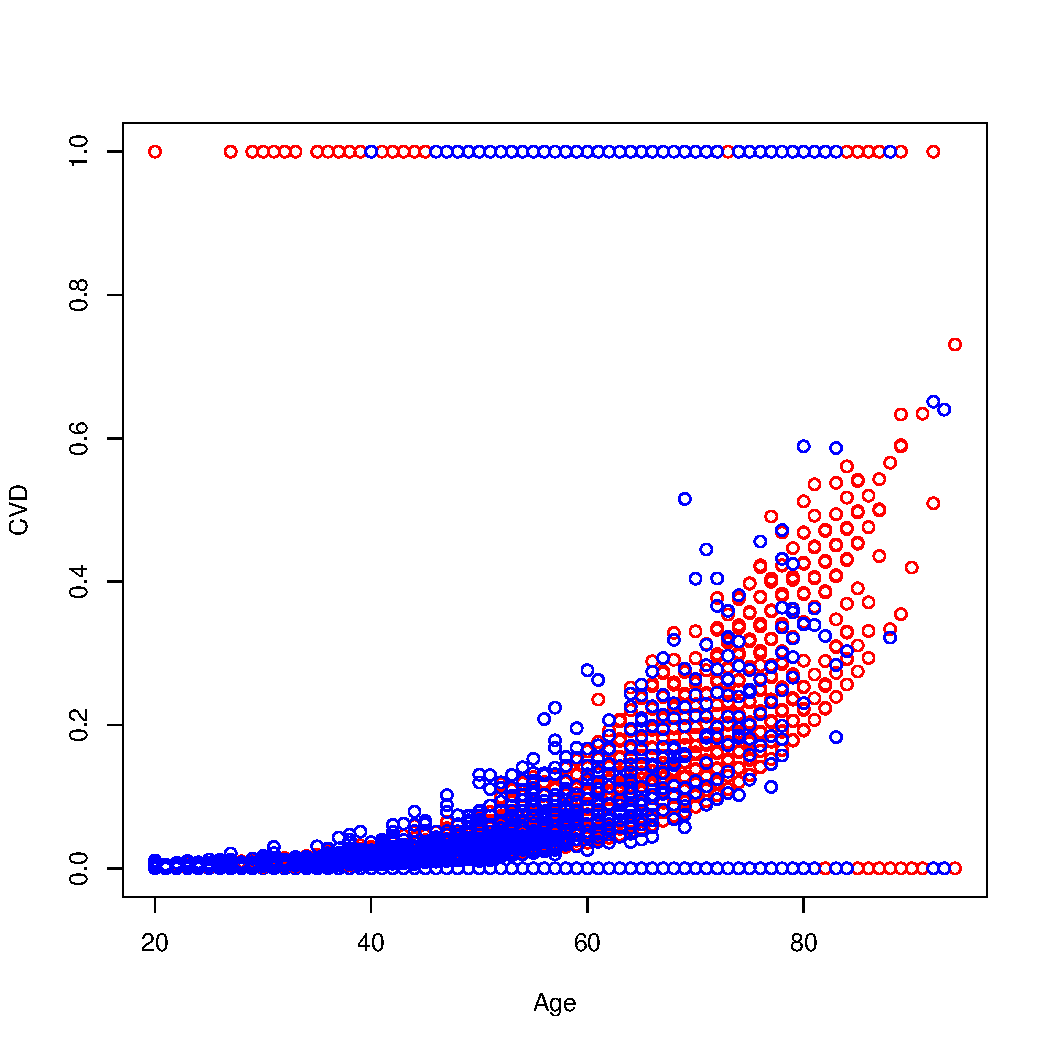
\includegraphics[width=\maxwidth]{figure/Plot_Analisi_ModelloPA-1} 
\end{knitrout}
    
    Il grafico non sembra mostrare differenze tra le due categorie di PA.

\clearpage


\section{Interazioni fra le variabili}
  Valutiamo se all'interno del modello ci sia la possibilità di interazioni
  fra le variabili. \par
  Consideriamo i casi nei quali le variabili come Smoke, Alchol, PA o Sex possano 
  interagire con le altre variabili, limitandoci unicamente nelle interazioni 
  del secondo ordine.
  
  \subsection{Smoke e Alchol}
  Analizziamo il caso nel quale il consumo di alchol, combinato con l'uso di 
  sigaretta, possa o meno aumentare le probabilità di CVD.
  
\begin{knitrout}
\definecolor{shadecolor}{rgb}{0.969, 0.969, 0.969}\color{fgcolor}\begin{kframe}
\begin{alltt}
\hlcom{#Modello con interazione: Smoke e Alchol}
\hlstd{fit.smokealchol} \hlkwb{<-} \hlkwd{glm}\hlstd{(nmc}\hlopt{$}\hlstd{cvd} \hlopt{~} \hlstd{nmc}\hlopt{$}\hlstd{sex}\hlopt{+}\hlstd{nmc}\hlopt{$}\hlstd{age}\hlopt{+}\hlstd{nmc}\hlopt{$}\hlstd{bmi}\hlopt{+}
                         \hlstd{nmc}\hlopt{$}\hlstd{fitness}\hlopt{+}\hlstd{nmc}\hlopt{$}\hlstd{smoke}\hlopt{+}
                         \hlstd{nmc}\hlopt{$}\hlstd{smoke}\hlopt{*}\hlstd{nmc}\hlopt{$}\hlstd{alc,}
                         \hlkwc{family}\hlstd{=binomial)}
\hlkwd{summary}\hlstd{(fit.smokealchol)}
\end{alltt}
\begin{verbatim}
## 
## Call:
## glm(formula = nmc$cvd ~ nmc$sex + nmc$age + nmc$bmi + nmc$fitness + 
##     nmc$smoke + nmc$smoke * nmc$alc, family = binomial)
## 
## Deviance Residuals: 
##     Min       1Q   Median       3Q      Max  
## -1.6094  -0.3392  -0.1936  -0.0952   3.6495  
## 
## Coefficients:
##                          Estimate Std. Error z value Pr(>|z|)    
## (Intercept)             -7.777741   0.409428 -18.997  < 2e-16 ***
## nmc$sexMale              0.800386   0.054612  14.656  < 2e-16 ***
## nmc$age                  0.092757   0.002449  37.869  < 2e-16 ***
## nmc$bmi                  0.233538   0.097010   2.407   0.0161 *  
## nmc$fitness             -0.183944   0.030378  -6.055  1.4e-09 ***
## nmc$smokeFormer          0.239303   0.425957   0.562   0.5743    
## nmc$smokeNO             -0.120962   0.395698  -0.306   0.7598    
## nmc$alc                  0.062892   0.142152   0.442   0.6582    
## nmc$smokeFormer:nmc$alc -0.223037   0.158794  -1.405   0.1602    
## nmc$smokeNO:nmc$alc     -0.094178   0.148217  -0.635   0.5252    
## ---
## Signif. codes:  0 '***' 0.001 '**' 0.01 '*' 0.05 '.' 0.1 ' ' 1
## 
## (Dispersion parameter for binomial family taken to be 1)
## 
##     Null deviance: 13400  on 33326  degrees of freedom
## Residual deviance: 10880  on 33317  degrees of freedom
## AIC: 10900
## 
## Number of Fisher Scoring iterations: 7
\end{verbatim}
\end{kframe}
\end{knitrout}
  
  I dati sembrano non mostrare l'interazione fra Smoke e Alchol.
  
  \subsection{Smoke e BMI}
  Vediamo se l'uso di sigaretta per una persona con un alto indice di massa 
  corporea possa aumentarne le probabilità.
  
\begin{knitrout}
\definecolor{shadecolor}{rgb}{0.969, 0.969, 0.969}\color{fgcolor}\begin{kframe}
\begin{alltt}
\hlcom{#Modello con interazione: Smoke e BMI}
\hlstd{fit.smokebmi} \hlkwb{<-} \hlkwd{glm}\hlstd{(nmc}\hlopt{$}\hlstd{cvd} \hlopt{~} \hlstd{nmc}\hlopt{$}\hlstd{sex}\hlopt{+}\hlstd{nmc}\hlopt{$}\hlstd{age}\hlopt{+}\hlstd{nmc}\hlopt{$}\hlstd{bmi}\hlopt{+}
                         \hlstd{nmc}\hlopt{$}\hlstd{fitness}\hlopt{+}\hlstd{nmc}\hlopt{$}\hlstd{smoke}\hlopt{+}
                         \hlstd{nmc}\hlopt{$}\hlstd{smoke}\hlopt{*}\hlstd{nmc}\hlopt{$}\hlstd{bmi,}
                         \hlkwc{family}\hlstd{=binomial)}
\hlkwd{summary}\hlstd{(fit.smokebmi)}
\end{alltt}
\begin{verbatim}
## 
## Call:
## glm(formula = nmc$cvd ~ nmc$sex + nmc$age + nmc$bmi + nmc$fitness + 
##     nmc$smoke + nmc$smoke * nmc$bmi, family = binomial)
## 
## Deviance Residuals: 
##     Min       1Q   Median       3Q      Max  
## -1.6167  -0.3389  -0.1923  -0.0938   3.6547  
## 
## Coefficients:
##                          Estimate Std. Error z value Pr(>|z|)    
## (Intercept)             -7.538233   0.187909 -40.116  < 2e-16 ***
## nmc$sexMale              0.789657   0.054027  14.616  < 2e-16 ***
## nmc$age                  0.092953   0.002438  38.128  < 2e-16 ***
## nmc$bmi                 -1.495180   0.726032  -2.059 0.039457 *  
## nmc$fitness             -0.186487   0.030356  -6.143 8.08e-10 ***
## nmc$smokeFormer         -0.400699   0.113377  -3.534 0.000409 ***
## nmc$smokeNO             -0.438392   0.107190  -4.090 4.32e-05 ***
## nmc$bmi:nmc$smokeFormer  1.667155   0.744567   2.239 0.025150 *  
## nmc$bmi:nmc$smokeNO      1.874406   0.734922   2.550 0.010757 *  
## ---
## Signif. codes:  0 '***' 0.001 '**' 0.01 '*' 0.05 '.' 0.1 ' ' 1
## 
## (Dispersion parameter for binomial family taken to be 1)
## 
##     Null deviance: 13400  on 33326  degrees of freedom
## Residual deviance: 10874  on 33318  degrees of freedom
## AIC: 10892
## 
## Number of Fisher Scoring iterations: 7
\end{verbatim}
\end{kframe}
\end{knitrout}
  
  A differenza di Smoke e Alchol, l'interazione tra Smoke e BMI 
  mostra un'interazione significativa, variando il valore stimato e diminuendo la 
  significatività della variabile BMI. In questo caso la variabile BMI assume 
  valore stimato negativo, influendo negativamente nella comparsa di CVD.
  
  \subsection{Alchol e BMI}
  Come per il caso di Smoke, verifichiamo se il consumo di alchol associato ad un
  maggior indice di massa corporea influisca nella probabilità di CVD.
  
\begin{knitrout}
\definecolor{shadecolor}{rgb}{0.969, 0.969, 0.969}\color{fgcolor}\begin{kframe}
\begin{alltt}
\hlcom{#Modello con interazione: Alchol e BMI}
\hlstd{fit.alcholbmi} \hlkwb{<-} \hlkwd{glm}\hlstd{(nmc}\hlopt{$}\hlstd{cvd} \hlopt{~} \hlstd{nmc}\hlopt{$}\hlstd{sex}\hlopt{+}\hlstd{nmc}\hlopt{$}\hlstd{age}\hlopt{+}\hlstd{nmc}\hlopt{$}\hlstd{bmi}\hlopt{+}
                         \hlstd{nmc}\hlopt{$}\hlstd{fitness}\hlopt{+}\hlstd{nmc}\hlopt{$}\hlstd{smoke}\hlopt{+}
                         \hlstd{nmc}\hlopt{$}\hlstd{alc}\hlopt{*}\hlstd{nmc}\hlopt{$}\hlstd{bmi,}
                         \hlkwc{family}\hlstd{=binomial)}
\hlkwd{summary}\hlstd{(fit.alcholbmi)}
\end{alltt}
\begin{verbatim}
## 
## Call:
## glm(formula = nmc$cvd ~ nmc$sex + nmc$age + nmc$bmi + nmc$fitness + 
##     nmc$smoke + nmc$alc * nmc$bmi, family = binomial)
## 
## Deviance Residuals: 
##     Min       1Q   Median       3Q      Max  
## -1.5941  -0.3386  -0.1936  -0.0950   3.6460  
## 
## Coefficients:
##                  Estimate Std. Error z value Pr(>|z|)    
## (Intercept)     -7.436723   0.211379 -35.182  < 2e-16 ***
## nmc$sexMale      0.798024   0.054655  14.601  < 2e-16 ***
## nmc$age          0.092645   0.002442  37.932  < 2e-16 ***
## nmc$bmi         -0.031850   0.282019  -0.113 0.910080    
## nmc$fitness     -0.184203   0.030379  -6.063 1.33e-09 ***
## nmc$smokeFormer -0.332279   0.111100  -2.991 0.002782 ** 
## nmc$smokeNO     -0.374629   0.106482  -3.518 0.000434 ***
## nmc$alc         -0.067192   0.037109  -1.811 0.070191 .  
## nmc$bmi:nmc$alc  0.120560   0.118070   1.021 0.307213    
## ---
## Signif. codes:  0 '***' 0.001 '**' 0.01 '*' 0.05 '.' 0.1 ' ' 1
## 
## (Dispersion parameter for binomial family taken to be 1)
## 
##     Null deviance: 13400  on 33326  degrees of freedom
## Residual deviance: 10882  on 33318  degrees of freedom
## AIC: 10900
## 
## Number of Fisher Scoring iterations: 7
\end{verbatim}
\end{kframe}
\end{knitrout}
  
  A differenza di Smoke*BMI, l'interazione tra Alchol e BMI non è supportata.
  
  \subsection{Sex e Smoke}
  Verifichiamo se l'utilizzo di sigaretta sia peggiorativo in uno dei due 
  sessi.
  
\begin{knitrout}
\definecolor{shadecolor}{rgb}{0.969, 0.969, 0.969}\color{fgcolor}\begin{kframe}
\begin{alltt}
\hlcom{#Modello con interazione: Sex e Smoke}
\hlstd{fit.sexsmoke} \hlkwb{<-} \hlkwd{glm}\hlstd{(nmc}\hlopt{$}\hlstd{cvd} \hlopt{~} \hlstd{nmc}\hlopt{$}\hlstd{sex}\hlopt{+}\hlstd{nmc}\hlopt{$}\hlstd{age}\hlopt{+}\hlstd{nmc}\hlopt{$}\hlstd{bmi}\hlopt{+}
                    \hlstd{nmc}\hlopt{$}\hlstd{fitness}\hlopt{+}\hlstd{nmc}\hlopt{$}\hlstd{smoke}\hlopt{+}
                    \hlstd{nmc}\hlopt{$}\hlstd{sex}\hlopt{*}\hlstd{nmc}\hlopt{$}\hlstd{smoke,}
                    \hlkwc{family}\hlstd{=binomial)}
\hlkwd{summary}\hlstd{(fit.sexsmoke)}
\end{alltt}
\begin{verbatim}
## 
## Call:
## glm(formula = nmc$cvd ~ nmc$sex + nmc$age + nmc$bmi + nmc$fitness + 
##     nmc$smoke + nmc$sex * nmc$smoke, family = binomial)
## 
## Deviance Residuals: 
##     Min       1Q   Median       3Q      Max  
## -1.5936  -0.3413  -0.1902  -0.0948   3.6359  
## 
## Coefficients:
##                              Estimate Std. Error z value Pr(>|z|)    
## (Intercept)                 -7.823919   0.218529 -35.803  < 2e-16 ***
## nmc$sexMale                  1.213811   0.200893   6.042 1.52e-09 ***
## nmc$age                      0.092548   0.002447  37.822  < 2e-16 ***
## nmc$bmi                      0.237345   0.096938   2.448   0.0143 *  
## nmc$fitness                 -0.182865   0.030381  -6.019 1.75e-09 ***
## nmc$smokeFormer             -0.168152   0.173095  -0.971   0.3313    
## nmc$smokeNO                 -0.086983   0.158493  -0.549   0.5831    
## nmc$sexMale:nmc$smokeFormer -0.332887   0.226013  -1.473   0.1408    
## nmc$sexMale:nmc$smokeNO     -0.513869   0.211536  -2.429   0.0151 *  
## ---
## Signif. codes:  0 '***' 0.001 '**' 0.01 '*' 0.05 '.' 0.1 ' ' 1
## 
## (Dispersion parameter for binomial family taken to be 1)
## 
##     Null deviance: 13400  on 33326  degrees of freedom
## Residual deviance: 10879  on 33318  degrees of freedom
## AIC: 10897
## 
## Number of Fisher Scoring iterations: 7
\end{verbatim}
\end{kframe}
\end{knitrout}
  
  L'interazione fra le variabili Sex e Smoke risulta non significativa.
  
  \subsection{Sex e Age}
  Analizziamo ora il caso nel quale l'aumento dell'età possa influenzare in
  maniera differente tra i due sessi.
  
\begin{knitrout}
\definecolor{shadecolor}{rgb}{0.969, 0.969, 0.969}\color{fgcolor}\begin{kframe}
\begin{alltt}
\hlcom{#Modello con interazione: Sex e Age}
\hlstd{fit.sexage} \hlkwb{<-} \hlkwd{glm}\hlstd{(nmc}\hlopt{$}\hlstd{cvd} \hlopt{~} \hlstd{nmc}\hlopt{$}\hlstd{sex}\hlopt{+}\hlstd{nmc}\hlopt{$}\hlstd{age}\hlopt{+}\hlstd{nmc}\hlopt{$}\hlstd{bmi}\hlopt{+}
                    \hlstd{nmc}\hlopt{$}\hlstd{fitness}\hlopt{+}\hlstd{nmc}\hlopt{$}\hlstd{smoke}\hlopt{+}
                    \hlstd{nmc}\hlopt{$}\hlstd{sex}\hlopt{*}\hlstd{nmc}\hlopt{$}\hlstd{age,}
                    \hlkwc{family}\hlstd{=binomial)}
\hlkwd{summary}\hlstd{(fit.sexage)}
\end{alltt}
\begin{verbatim}
## 
## Call:
## glm(formula = nmc$cvd ~ nmc$sex + nmc$age + nmc$bmi + nmc$fitness + 
##     nmc$smoke + nmc$sex * nmc$age, family = binomial)
## 
## Deviance Residuals: 
##     Min       1Q   Median       3Q      Max  
## -1.5257  -0.3426  -0.1892  -0.0925   3.7386  
## 
## Coefficients:
##                      Estimate Std. Error z value Pr(>|z|)    
## (Intercept)         -8.072593   0.247550 -32.610  < 2e-16 ***
## nmc$sexMale          1.686372   0.306886   5.495 3.90e-08 ***
## nmc$age              0.100329   0.003529  28.427  < 2e-16 ***
## nmc$bmi              0.233344   0.096960   2.407 0.016102 *  
## nmc$fitness         -0.185576   0.030249  -6.135 8.52e-10 ***
## nmc$smokeFormer     -0.328928   0.111095  -2.961 0.003069 ** 
## nmc$smokeNO         -0.364822   0.105629  -3.454 0.000553 ***
## nmc$sexMale:nmc$age -0.014186   0.004760  -2.980 0.002879 ** 
## ---
## Signif. codes:  0 '***' 0.001 '**' 0.01 '*' 0.05 '.' 0.1 ' ' 1
## 
## (Dispersion parameter for binomial family taken to be 1)
## 
##     Null deviance: 13400  on 33326  degrees of freedom
## Residual deviance: 10877  on 33319  degrees of freedom
## AIC: 10893
## 
## Number of Fisher Scoring iterations: 7
\end{verbatim}
\end{kframe}
\end{knitrout}
  
  Contrariamente a quello che ci si poteva aspettare, esiste un interazione 
  significativa tra la variabile Sex e Age. Per il sesso maschile con l'aumentare
  dell'età ha, anche se piccola, una riduzione nella probabilità di CVD. \par
  Analizzeremo successivamente se questa interazione può risultare utile ai fini
  del nostro problema.
  
  \subsection{PA e Age}
  Verifichiamo se l'attività fisica di un individuo è influenzata in base
  alla sua età.
\begin{knitrout}
\definecolor{shadecolor}{rgb}{0.969, 0.969, 0.969}\color{fgcolor}\begin{kframe}
\begin{alltt}
\hlcom{#Modello con interazione PA e Age}
\hlstd{fit.sexsmoke} \hlkwb{<-} \hlkwd{glm}\hlstd{(nmc}\hlopt{$}\hlstd{cvd} \hlopt{~} \hlstd{nmc}\hlopt{$}\hlstd{sex}\hlopt{+}\hlstd{nmc}\hlopt{$}\hlstd{age}\hlopt{+}\hlstd{nmc}\hlopt{$}\hlstd{bmi}\hlopt{+}
                    \hlstd{nmc}\hlopt{$}\hlstd{fitness}\hlopt{+}\hlstd{nmc}\hlopt{$}\hlstd{smoke}\hlopt{+}
                    \hlstd{nmc}\hlopt{$}\hlstd{pa}\hlopt{*}\hlstd{nmc}\hlopt{$}\hlstd{age,}
                    \hlkwc{family}\hlstd{=binomial)}
\hlkwd{summary}\hlstd{(fit.sexsmoke)}
\end{alltt}
\begin{verbatim}
## 
## Call:
## glm(formula = nmc$cvd ~ nmc$sex + nmc$age + nmc$bmi + nmc$fitness + 
##     nmc$smoke + nmc$pa * nmc$age, family = binomial)
## 
## Deviance Residuals: 
##     Min       1Q   Median       3Q      Max  
## -1.6223  -0.3380  -0.1931  -0.0944   3.6547  
## 
## Coefficients:
##                  Estimate Std. Error z value Pr(>|z|)    
## (Intercept)     -7.637524   0.196623 -38.844  < 2e-16 ***
## nmc$sexMale      0.785270   0.054030  14.534  < 2e-16 ***
## nmc$age          0.093182   0.002543  36.636  < 2e-16 ***
## nmc$bmi          0.239306   0.096938   2.469 0.013563 *  
## nmc$fitness     -0.183966   0.031043  -5.926  3.1e-09 ***
## nmc$smokeFormer -0.331027   0.111137  -2.979 0.002896 ** 
## nmc$smokeNO     -0.351321   0.105525  -3.329 0.000871 ***
## nmc$pa           0.150329   0.532956   0.282 0.777893    
## nmc$age:nmc$pa  -0.001873   0.008691  -0.216 0.829356    
## ---
## Signif. codes:  0 '***' 0.001 '**' 0.01 '*' 0.05 '.' 0.1 ' ' 1
## 
## (Dispersion parameter for binomial family taken to be 1)
## 
##     Null deviance: 13400  on 33326  degrees of freedom
## Residual deviance: 10886  on 33318  degrees of freedom
## AIC: 10904
## 
## Number of Fisher Scoring iterations: 7
\end{verbatim}
\end{kframe}
\end{knitrout}
  
  Non è verificata l'interazione fra le variabili PA e Age.
  
  \subsection{PA e Fitness}
  Analliziamo il caso nel quale l'attività fisica e lo stato di salute di un
  individuo possano aumentare le probabilità di CVD.
  
\begin{knitrout}
\definecolor{shadecolor}{rgb}{0.969, 0.969, 0.969}\color{fgcolor}\begin{kframe}
\begin{alltt}
\hlcom{#Modello con interazione PA e Fitness}
\hlstd{fit.sexsmoke} \hlkwb{<-} \hlkwd{glm}\hlstd{(nmc}\hlopt{$}\hlstd{cvd} \hlopt{~} \hlstd{nmc}\hlopt{$}\hlstd{sex}\hlopt{+}\hlstd{nmc}\hlopt{$}\hlstd{age}\hlopt{+}\hlstd{nmc}\hlopt{$}\hlstd{bmi}\hlopt{+}
                    \hlstd{nmc}\hlopt{$}\hlstd{fitness}\hlopt{+}\hlstd{nmc}\hlopt{$}\hlstd{smoke}\hlopt{+}
                    \hlstd{nmc}\hlopt{$}\hlstd{pa}\hlopt{*}\hlstd{nmc}\hlopt{$}\hlstd{fitness,}
                    \hlkwc{family}\hlstd{=binomial)}
\hlkwd{summary}\hlstd{(fit.sexsmoke)}
\end{alltt}
\begin{verbatim}
## 
## Call:
## glm(formula = nmc$cvd ~ nmc$sex + nmc$age + nmc$bmi + nmc$fitness + 
##     nmc$smoke + nmc$pa * nmc$fitness, family = binomial)
## 
## Deviance Residuals: 
##     Min       1Q   Median       3Q      Max  
## -1.6172  -0.3387  -0.1939  -0.0944   3.6542  
## 
## Coefficients:
##                    Estimate Std. Error z value Pr(>|z|)    
## (Intercept)        -7.66807    0.19391 -39.545  < 2e-16 ***
## nmc$sexMale         0.78531    0.05400  14.543  < 2e-16 ***
## nmc$age             0.09301    0.00244  38.121  < 2e-16 ***
## nmc$bmi             0.23582    0.09706   2.430 0.015113 *  
## nmc$fitness        -0.17257    0.03220  -5.358  8.4e-08 ***
## nmc$smokeFormer    -0.33083    0.11115  -2.976 0.002917 ** 
## nmc$smokeNO        -0.34965    0.10557  -3.312 0.000926 ***
## nmc$pa              0.44155    0.31777   1.390 0.164666    
## nmc$fitness:nmc$pa -0.14624    0.10964  -1.334 0.182252    
## ---
## Signif. codes:  0 '***' 0.001 '**' 0.01 '*' 0.05 '.' 0.1 ' ' 1
## 
## (Dispersion parameter for binomial family taken to be 1)
## 
##     Null deviance: 13400  on 33326  degrees of freedom
## Residual deviance: 10884  on 33318  degrees of freedom
## AIC: 10902
## 
## Number of Fisher Scoring iterations: 7
\end{verbatim}
\end{kframe}
\end{knitrout}
  
  Il modello mostra come non ci sia interazione fra le variabili PA e Fitness.
  
  \subsection{Modello con interazioni}
  Analizziamo ora il modello con solo variabili significative aggiungendo
  le interazioni che precedentemente abbiamo valutato come significative.\par
  Il modello da valutare sarà quindi:\\
  Modello: CVD $\sim$ Sex + Age + BMI + Fitness + Smoke + Sex*Age + Smoke*BMI.
  
\begin{knitrout}
\definecolor{shadecolor}{rgb}{0.969, 0.969, 0.969}\color{fgcolor}\begin{kframe}
\begin{alltt}
\hlcom{#Modello con interazione: Sex*Age + Smoke*BMI}
\hlstd{fit.int} \hlkwb{<-} \hlkwd{glm}\hlstd{(nmc}\hlopt{$}\hlstd{cvd} \hlopt{~} \hlstd{nmc}\hlopt{$}\hlstd{sex}\hlopt{+}\hlstd{nmc}\hlopt{$}\hlstd{age}\hlopt{+}\hlstd{nmc}\hlopt{$}\hlstd{bmi}\hlopt{+}
                 \hlstd{nmc}\hlopt{$}\hlstd{fitness}\hlopt{+}\hlstd{nmc}\hlopt{$}\hlstd{smoke}\hlopt{+}
                 \hlstd{nmc}\hlopt{$}\hlstd{sex}\hlopt{*}\hlstd{nmc}\hlopt{$}\hlstd{age}\hlopt{+}
                 \hlstd{nmc}\hlopt{$}\hlstd{smoke}\hlopt{*}\hlstd{nmc}\hlopt{$}\hlstd{bmi,}
                 \hlkwc{family}\hlstd{=binomial)}
\hlkwd{summary}\hlstd{(fit.int)}
\end{alltt}
\begin{verbatim}
## 
## Call:
## glm(formula = nmc$cvd ~ nmc$sex + nmc$age + nmc$bmi + nmc$fitness + 
##     nmc$smoke + nmc$sex * nmc$age + nmc$smoke * nmc$bmi, family = binomial)
## 
## Deviance Residuals: 
##     Min       1Q   Median       3Q      Max  
## -1.5214  -0.3437  -0.1885  -0.0913   3.7412  
## 
## Coefficients:
##                          Estimate Std. Error z value Pr(>|z|)    
## (Intercept)             -7.994945   0.248199 -32.212  < 2e-16 ***
## nmc$sexMale              1.684991   0.307149   5.486 4.11e-08 ***
## nmc$age                  0.100260   0.003532  28.386  < 2e-16 ***
## nmc$bmi                 -1.494470   0.726361  -2.057 0.039641 *  
## nmc$fitness             -0.185813   0.030262  -6.140 8.24e-10 ***
## nmc$smokeFormer         -0.396574   0.113345  -3.499 0.000467 ***
## nmc$smokeNO             -0.450336   0.107284  -4.198 2.70e-05 ***
## nmc$sexMale:nmc$age     -0.014114   0.004764  -2.963 0.003050 ** 
## nmc$bmi:nmc$smokeFormer  1.656064   0.744884   2.223 0.026199 *  
## nmc$bmi:nmc$smokeNO      1.867843   0.735274   2.540 0.011075 *  
## ---
## Signif. codes:  0 '***' 0.001 '**' 0.01 '*' 0.05 '.' 0.1 ' ' 1
## 
## (Dispersion parameter for binomial family taken to be 1)
## 
##     Null deviance: 13400  on 33326  degrees of freedom
## Residual deviance: 10866  on 33317  degrees of freedom
## AIC: 10886
## 
## Number of Fisher Scoring iterations: 7
\end{verbatim}
\end{kframe}
\end{knitrout}

  \subsection{Commento}
    Nonostante il modello con le due interazioni Smoke*BMI e Sex*Age risulti
    significativo, vediamo come questo si comporti in maniera differente dalle
    valutazioni che abbiamo analizzato precedentemente.\par
    Il modello con interazioni mostra una minor probabilità per un individuo che
    fuma e con alto indice di massa corporea, o come un individuo di sesso
    maschile abbia una minima riduzione di probabilità con l'aumentare dell'
    età.\par
    Inoltre il significato della variabile BMI varia rispetto al modello con 
    solo variabili significative e al modello con la sola regressione logistica 
    semplice, diminuendone anche la significatività. \par
    Decido quindi di non considerare questo modello perchè, oltre ad aumentarne 
    il grado, non fornisce un contributo decisivo per il nostro problema,
    andando contro anche alle analisi che fino a qui abbiamo valutato. \par

\clearpage


\section{Selezione del Modello}
  Utilizziamo adesso i metodi Backward, Forward e Both basati sui criteri di 
  penalizzazione AIC e BIC per la selezione del modello.\par
  Per eseguire le varie procedure, prenderemo in considerazione la formula base 
  con solo l'intercetta e il modello che comprende tutte le variabili fornite 
  dal dataset, senza interazioni.
  
\begin{knitrout}
\definecolor{shadecolor}{rgb}{0.969, 0.969, 0.969}\color{fgcolor}\begin{kframe}
\begin{alltt}
\hlcom{#Iniziliazziamo la formula base con intercetta}
\hlstd{fit.0} \hlkwb{<-} \hlkwd{glm}\hlstd{(nmc}\hlopt{$}\hlstd{cvd} \hlopt{~} \hlnum{1}\hlstd{,} \hlkwc{family}\hlstd{=} \hlstr{"binomial"}\hlstd{)}
\end{alltt}
\end{kframe}
\end{knitrout}

   \subsection{Backward}
      Verifichiamo le formule della procedura Backward con AIC e BIC.
        \subsubsection{AIC}
\begin{knitrout}
\definecolor{shadecolor}{rgb}{0.969, 0.969, 0.969}\color{fgcolor}\begin{kframe}
\begin{alltt}
\hlcom{#Backward: AIC}
\hlstd{backward.AIC} \hlkwb{<-} \hlkwd{step}\hlstd{(fit.all,} \hlkwc{direction}\hlstd{=}\hlstr{"backward"}\hlstd{,} \hlkwc{k}\hlstd{=}\hlnum{2}\hlstd{)}
\end{alltt}
\begin{verbatim}
## Start:  AIC=10901.21
## nmc$cvd ~ nmc$sex + nmc$age + nmc$bmi + nmc$fitness + nmc$pa + 
##     nmc$smoke + nmc$alc
## 
##               Df Deviance   AIC
## - nmc$pa       1    10883 10899
## <none>              10883 10901
## - nmc$alc      1    10886 10902
## - nmc$bmi      1    10889 10905
## - nmc$smoke    2    10895 10909
## - nmc$fitness  1    10917 10933
## - nmc$sex      1    11097 11113
## - nmc$age      1    13043 13059
## 
## Step:  AIC=10899.32
## nmc$cvd ~ nmc$sex + nmc$age + nmc$bmi + nmc$fitness + nmc$smoke + 
##     nmc$alc
## 
##               Df Deviance   AIC
## <none>              10883 10899
## - nmc$alc      1    10886 10900
## - nmc$bmi      1    10889 10903
## - nmc$smoke    2    10895 10907
## - nmc$fitness  1    10920 10934
## - nmc$sex      1    11098 11112
## - nmc$age      1    13045 13059
\end{verbatim}
\begin{alltt}
\hlkwd{formula}\hlstd{(backward.AIC)}
\end{alltt}
\begin{verbatim}
## nmc$cvd ~ nmc$sex + nmc$age + nmc$bmi + nmc$fitness + nmc$smoke + 
##     nmc$alc
\end{verbatim}
\begin{alltt}
\hlkwd{summary}\hlstd{(backward.AIC)}
\end{alltt}
\begin{verbatim}
## 
## Call:
## glm(formula = nmc$cvd ~ nmc$sex + nmc$age + nmc$bmi + nmc$fitness + 
##     nmc$smoke + nmc$alc, family = binomial)
## 
## Deviance Residuals: 
##     Min       1Q   Median       3Q      Max  
## -1.5978  -0.3371  -0.1941  -0.0950   3.6471  
## 
## Coefficients:
##                  Estimate Std. Error z value Pr(>|z|)    
## (Intercept)     -7.462934   0.209921 -35.551  < 2e-16 ***
## nmc$sexMale      0.799887   0.054643  14.638  < 2e-16 ***
## nmc$age          0.092640   0.002442  37.930  < 2e-16 ***
## nmc$bmi          0.235857   0.096958   2.433 0.014992 *  
## nmc$fitness     -0.183877   0.030378  -6.053 1.42e-09 ***
## nmc$smokeFormer -0.332592   0.111097  -2.994 0.002756 ** 
## nmc$smokeNO     -0.374525   0.106476  -3.517 0.000436 ***
## nmc$alc         -0.056553   0.035625  -1.587 0.112413    
## ---
## Signif. codes:  0 '***' 0.001 '**' 0.01 '*' 0.05 '.' 0.1 ' ' 1
## 
## (Dispersion parameter for binomial family taken to be 1)
## 
##     Null deviance: 13400  on 33326  degrees of freedom
## Residual deviance: 10883  on 33319  degrees of freedom
## AIC: 10899
## 
## Number of Fisher Scoring iterations: 7
\end{verbatim}
\end{kframe}
\end{knitrout}
          
        \subsubsection{BIC}
\begin{knitrout}
\definecolor{shadecolor}{rgb}{0.969, 0.969, 0.969}\color{fgcolor}\begin{kframe}
\begin{alltt}
\hlcom{#Backward: BIC }
\hlstd{backward.BIC} \hlkwb{<-} \hlkwd{step}\hlstd{(fit.all,} \hlkwc{direction}\hlstd{=}\hlstr{"backward"}\hlstd{,}
                    \hlkwc{k}\hlstd{=}\hlkwd{log}\hlstd{(}\hlkwd{length}\hlstd{(nmc}\hlopt{$}\hlstd{cvd)))}
\end{alltt}
\begin{verbatim}
## Start:  AIC=10976.94
## nmc$cvd ~ nmc$sex + nmc$age + nmc$bmi + nmc$fitness + nmc$pa + 
##     nmc$smoke + nmc$alc
## 
##               Df Deviance   AIC
## - nmc$pa       1    10883 10967
## - nmc$smoke    2    10895 10968
## - nmc$alc      1    10886 10969
## - nmc$bmi      1    10889 10972
## <none>              10883 10977
## - nmc$fitness  1    10917 11001
## - nmc$sex      1    11097 11180
## - nmc$age      1    13043 13127
## 
## Step:  AIC=10966.63
## nmc$cvd ~ nmc$sex + nmc$age + nmc$bmi + nmc$fitness + nmc$smoke + 
##     nmc$alc
## 
##               Df Deviance   AIC
## - nmc$smoke    2    10895 10957
## - nmc$alc      1    10886 10959
## - nmc$bmi      1    10889 10962
## <none>              10883 10967
## - nmc$fitness  1    10920 10993
## - nmc$sex      1    11098 11170
## - nmc$age      1    13045 13118
## 
## Step:  AIC=10957.36
## nmc$cvd ~ nmc$sex + nmc$age + nmc$bmi + nmc$fitness + nmc$alc
## 
##               Df Deviance   AIC
## - nmc$alc      1    10896 10948
## - nmc$bmi      1    10900 10952
## <none>              10895 10957
## - nmc$fitness  1    10936 10988
## - nmc$sex      1    11114 11167
## - nmc$age      1    13050 13102
## 
## Step:  AIC=10948.37
## nmc$cvd ~ nmc$sex + nmc$age + nmc$bmi + nmc$fitness
## 
##               Df Deviance   AIC
## - nmc$bmi      1    10902 10943
## <none>              10896 10948
## - nmc$fitness  1    10938 10979
## - nmc$sex      1    11117 11159
## - nmc$age      1    13059 13100
## 
## Step:  AIC=10943.43
## nmc$cvd ~ nmc$sex + nmc$age + nmc$fitness
## 
##               Df Deviance   AIC
## <none>              10902 10943
## - nmc$fitness  1    10952 10983
## - nmc$sex      1    11120 11151
## - nmc$age      1    13073 13104
\end{verbatim}
\begin{alltt}
\hlkwd{formula}\hlstd{(backward.BIC)}
\end{alltt}
\begin{verbatim}
## nmc$cvd ~ nmc$sex + nmc$age + nmc$fitness
\end{verbatim}
\begin{alltt}
\hlkwd{summary}\hlstd{(backward.BIC)}
\end{alltt}
\begin{verbatim}
## 
## Call:
## glm(formula = nmc$cvd ~ nmc$sex + nmc$age + nmc$fitness, family = binomial)
## 
## Deviance Residuals: 
##     Min       1Q   Median       3Q      Max  
## -1.6340  -0.3381  -0.1940  -0.0966   3.6228  
## 
## Coefficients:
##              Estimate Std. Error z value Pr(>|z|)    
## (Intercept) -7.771416   0.170954  -45.46  < 2e-16 ***
## nmc$sexMale  0.783860   0.053038   14.78  < 2e-16 ***
## nmc$age      0.091980   0.002398   38.35  < 2e-16 ***
## nmc$fitness -0.209655   0.029570   -7.09 1.34e-12 ***
## ---
## Signif. codes:  0 '***' 0.001 '**' 0.01 '*' 0.05 '.' 0.1 ' ' 1
## 
## (Dispersion parameter for binomial family taken to be 1)
## 
##     Null deviance: 13400  on 33326  degrees of freedom
## Residual deviance: 10902  on 33323  degrees of freedom
## AIC: 10910
## 
## Number of Fisher Scoring iterations: 7
\end{verbatim}
\end{kframe}
\end{knitrout}
          
    \subsection{Forward} 
      Verifichiamo adesso le formule della procedura Forward con AIC e BIC.
        \subsubsection{AIC}
\begin{knitrout}
\definecolor{shadecolor}{rgb}{0.969, 0.969, 0.969}\color{fgcolor}\begin{kframe}
\begin{alltt}
\hlcom{#Forward: AIC}
\hlstd{forward.AIC} \hlkwb{<-} \hlkwd{step}\hlstd{(fit.0,} \hlkwc{scope}\hlstd{=}\hlkwd{formula}\hlstd{(fit.all),}
                   \hlkwc{direction}\hlstd{=}\hlstr{"forward"}\hlstd{,} \hlkwc{k}\hlstd{=}\hlnum{2}\hlstd{,} \hlkwc{trace}\hlstd{=}\hlnum{FALSE}\hlstd{)}
\hlkwd{formula}\hlstd{(forward.AIC)}
\end{alltt}
\begin{verbatim}
## nmc$cvd ~ nmc$age + nmc$sex + nmc$fitness + nmc$smoke + nmc$bmi + 
##     nmc$alc
\end{verbatim}
\begin{alltt}
\hlkwd{summary}\hlstd{(forward.AIC)}
\end{alltt}
\begin{verbatim}
## 
## Call:
## glm(formula = nmc$cvd ~ nmc$age + nmc$sex + nmc$fitness + nmc$smoke + 
##     nmc$bmi + nmc$alc, family = "binomial")
## 
## Deviance Residuals: 
##     Min       1Q   Median       3Q      Max  
## -1.5978  -0.3371  -0.1941  -0.0950   3.6471  
## 
## Coefficients:
##                  Estimate Std. Error z value Pr(>|z|)    
## (Intercept)     -7.462934   0.209921 -35.551  < 2e-16 ***
## nmc$age          0.092640   0.002442  37.930  < 2e-16 ***
## nmc$sexMale      0.799887   0.054643  14.638  < 2e-16 ***
## nmc$fitness     -0.183877   0.030378  -6.053 1.42e-09 ***
## nmc$smokeFormer -0.332592   0.111097  -2.994 0.002756 ** 
## nmc$smokeNO     -0.374525   0.106476  -3.517 0.000436 ***
## nmc$bmi          0.235857   0.096958   2.433 0.014992 *  
## nmc$alc         -0.056553   0.035625  -1.587 0.112413    
## ---
## Signif. codes:  0 '***' 0.001 '**' 0.01 '*' 0.05 '.' 0.1 ' ' 1
## 
## (Dispersion parameter for binomial family taken to be 1)
## 
##     Null deviance: 13400  on 33326  degrees of freedom
## Residual deviance: 10883  on 33319  degrees of freedom
## AIC: 10899
## 
## Number of Fisher Scoring iterations: 7
\end{verbatim}
\end{kframe}
\end{knitrout}
          
        \subsubsection{BIC}
\begin{knitrout}
\definecolor{shadecolor}{rgb}{0.969, 0.969, 0.969}\color{fgcolor}\begin{kframe}
\begin{alltt}
\hlcom{#Forward: BIC}
\hlstd{forward.BIC} \hlkwb{<-} \hlkwd{step}\hlstd{(fit.0,} \hlkwc{scope}\hlstd{=}\hlkwd{formula}\hlstd{(fit.all),}
                   \hlkwc{direction}\hlstd{=}\hlstr{"forward"}\hlstd{,}
                   \hlkwc{k}\hlstd{=}\hlkwd{log}\hlstd{(}\hlkwd{length}\hlstd{(nmc}\hlopt{$}\hlstd{cvd)),}
                   \hlkwc{trace}\hlstd{=}\hlnum{FALSE}\hlstd{)}
\hlkwd{formula}\hlstd{(forward.BIC)}
\end{alltt}
\begin{verbatim}
## nmc$cvd ~ nmc$age + nmc$sex + nmc$fitness
\end{verbatim}
\begin{alltt}
\hlkwd{summary}\hlstd{(forward.BIC)}
\end{alltt}
\begin{verbatim}
## 
## Call:
## glm(formula = nmc$cvd ~ nmc$age + nmc$sex + nmc$fitness, family = "binomial")
## 
## Deviance Residuals: 
##     Min       1Q   Median       3Q      Max  
## -1.6340  -0.3381  -0.1940  -0.0966   3.6228  
## 
## Coefficients:
##              Estimate Std. Error z value Pr(>|z|)    
## (Intercept) -7.771416   0.170954  -45.46  < 2e-16 ***
## nmc$age      0.091980   0.002398   38.35  < 2e-16 ***
## nmc$sexMale  0.783860   0.053038   14.78  < 2e-16 ***
## nmc$fitness -0.209655   0.029570   -7.09 1.34e-12 ***
## ---
## Signif. codes:  0 '***' 0.001 '**' 0.01 '*' 0.05 '.' 0.1 ' ' 1
## 
## (Dispersion parameter for binomial family taken to be 1)
## 
##     Null deviance: 13400  on 33326  degrees of freedom
## Residual deviance: 10902  on 33323  degrees of freedom
## AIC: 10910
## 
## Number of Fisher Scoring iterations: 7
\end{verbatim}
\end{kframe}
\end{knitrout}
          
    \subsection{Both}
      Infine vediamo le formule della procedura Both con AIC e BIC.
        \subsubsection{AIC}
\begin{knitrout}
\definecolor{shadecolor}{rgb}{0.969, 0.969, 0.969}\color{fgcolor}\begin{kframe}
\begin{alltt}
\hlcom{#Both: AIC }
\hlstd{both.AIC} \hlkwb{<-} \hlkwd{step}\hlstd{(fit.0,} \hlkwc{scope}\hlstd{=}\hlkwd{formula}\hlstd{(fit.all),}
                 \hlkwc{direction}\hlstd{=}\hlstr{"both"}\hlstd{,}
                 \hlkwc{k}\hlstd{=}\hlnum{2}\hlstd{,} \hlkwc{trace}\hlstd{=}\hlnum{FALSE}\hlstd{)}
\hlkwd{formula}\hlstd{(both.AIC)}
\end{alltt}
\begin{verbatim}
## nmc$cvd ~ nmc$age + nmc$sex + nmc$fitness + nmc$smoke + nmc$bmi + 
##     nmc$alc
\end{verbatim}
\begin{alltt}
\hlkwd{summary}\hlstd{(both.AIC)}
\end{alltt}
\begin{verbatim}
## 
## Call:
## glm(formula = nmc$cvd ~ nmc$age + nmc$sex + nmc$fitness + nmc$smoke + 
##     nmc$bmi + nmc$alc, family = "binomial")
## 
## Deviance Residuals: 
##     Min       1Q   Median       3Q      Max  
## -1.5978  -0.3371  -0.1941  -0.0950   3.6471  
## 
## Coefficients:
##                  Estimate Std. Error z value Pr(>|z|)    
## (Intercept)     -7.462934   0.209921 -35.551  < 2e-16 ***
## nmc$age          0.092640   0.002442  37.930  < 2e-16 ***
## nmc$sexMale      0.799887   0.054643  14.638  < 2e-16 ***
## nmc$fitness     -0.183877   0.030378  -6.053 1.42e-09 ***
## nmc$smokeFormer -0.332592   0.111097  -2.994 0.002756 ** 
## nmc$smokeNO     -0.374525   0.106476  -3.517 0.000436 ***
## nmc$bmi          0.235857   0.096958   2.433 0.014992 *  
## nmc$alc         -0.056553   0.035625  -1.587 0.112413    
## ---
## Signif. codes:  0 '***' 0.001 '**' 0.01 '*' 0.05 '.' 0.1 ' ' 1
## 
## (Dispersion parameter for binomial family taken to be 1)
## 
##     Null deviance: 13400  on 33326  degrees of freedom
## Residual deviance: 10883  on 33319  degrees of freedom
## AIC: 10899
## 
## Number of Fisher Scoring iterations: 7
\end{verbatim}
\end{kframe}
\end{knitrout}
          
        \subsubsection{BIC}
\begin{knitrout}
\definecolor{shadecolor}{rgb}{0.969, 0.969, 0.969}\color{fgcolor}\begin{kframe}
\begin{alltt}
\hlcom{#Bot: BIC}
\hlstd{both.BIC} \hlkwb{<-} \hlkwd{step}\hlstd{(fit.0,} \hlkwc{scope}\hlstd{=}\hlkwd{formula}\hlstd{(fit.all),}
                 \hlkwc{direction}\hlstd{=}\hlstr{"both"}\hlstd{,}
                 \hlkwc{k}\hlstd{=}\hlkwd{log}\hlstd{(}\hlkwd{length}\hlstd{(nmc}\hlopt{$}\hlstd{cvd)),}
                 \hlkwc{trace}\hlstd{=}\hlnum{FALSE}\hlstd{)}
\hlkwd{formula}\hlstd{(both.BIC)}
\end{alltt}
\begin{verbatim}
## nmc$cvd ~ nmc$age + nmc$sex + nmc$fitness
\end{verbatim}
\begin{alltt}
\hlkwd{summary}\hlstd{(both.BIC)}
\end{alltt}
\begin{verbatim}
## 
## Call:
## glm(formula = nmc$cvd ~ nmc$age + nmc$sex + nmc$fitness, family = "binomial")
## 
## Deviance Residuals: 
##     Min       1Q   Median       3Q      Max  
## -1.6340  -0.3381  -0.1940  -0.0966   3.6228  
## 
## Coefficients:
##              Estimate Std. Error z value Pr(>|z|)    
## (Intercept) -7.771416   0.170954  -45.46  < 2e-16 ***
## nmc$age      0.091980   0.002398   38.35  < 2e-16 ***
## nmc$sexMale  0.783860   0.053038   14.78  < 2e-16 ***
## nmc$fitness -0.209655   0.029570   -7.09 1.34e-12 ***
## ---
## Signif. codes:  0 '***' 0.001 '**' 0.01 '*' 0.05 '.' 0.1 ' ' 1
## 
## (Dispersion parameter for binomial family taken to be 1)
## 
##     Null deviance: 13400  on 33326  degrees of freedom
## Residual deviance: 10902  on 33323  degrees of freedom
## AIC: 10910
## 
## Number of Fisher Scoring iterations: 7
\end{verbatim}
\end{kframe}
\end{knitrout}
    
    \subsection{Commento}
      Le formule ottenute dalle tre procedure sono:
        \begin{itemize}
          \item Le procedure FORWARD, BACKWARD e BOTH AIC: \\
                CVD $\sim$ Age + Sex + Fitness + Smoke + BMI + Alchol
          \item Le procedure FORWARD, BACKWARD e BOTH BIC: \\
                CVD $\sim$ Age + Sex + Fitness
        \end{itemize}
        
      In questo caso, basandomi sulle procedure AIC e BIC, 
      seleziono il risultato dalla procedura AIC ed elimino, secondo il
      $\emph{p-value}$, la variabile non significativa Alchol, ottenendo un modello
      che si pone in mezzo alle procedure AIC e BIC. \par
      Il modello risultate da questa analisi risulta essere quello analizzato
      nel capitolo delle regressioni logistiche multiple. \par
      Modello: CVD $\sim$ Sex + Age + Fitness + Smoke + BMI. \par

\clearpage


\section{Test sul Modello}
  Verifichiamo adesso come il modello tende a calcolare la probabilità per un         campione di individui.
  
  \subsection{Age}
    Calcoliamo la probabilità di un ragazzo di 26 anni e di Uomo di 42 anni, 
    entrambi fumatori (Smoke:Current), con BMI pari a 25(BMI 0) che stanno male 
    (Fitness 2).
      
\begin{knitrout}
\definecolor{shadecolor}{rgb}{0.969, 0.969, 0.969}\color{fgcolor}\begin{kframe}
\begin{alltt}
\hlcom{#Dato ragazzo}
\hlcom{#Intercetta: 1, SexMale: 1, Age: 26, BMI: 0, Fitness: 2, }
\hlcom{#Smoke:Former: 0, Smoke:NO: 0 }
\hlstd{t.age.boy} \hlkwb{<-} \hlkwd{c}\hlstd{(}\hlnum{1}\hlstd{,} \hlnum{1}\hlstd{,} \hlnum{26}\hlstd{,} \hlnum{0}\hlstd{,} \hlnum{2}\hlstd{,} \hlnum{0}\hlstd{,} \hlnum{0}\hlstd{)}

\hlcom{#Dato Uomo}
\hlcom{#Intercetta: 1, SexMale: 1, Age: 42, BMI: 0, Fitness: 2, }
\hlcom{#Smoke:Former: 0, Smoke:NO: 0 }
\hlstd{t.age.man} \hlkwb{<-} \hlkwd{c}\hlstd{(}\hlnum{1}\hlstd{,} \hlnum{1}\hlstd{,} \hlnum{42}\hlstd{,} \hlnum{0}\hlstd{,} \hlnum{2}\hlstd{,} \hlnum{0}\hlstd{,} \hlnum{0}\hlstd{)}
\end{alltt}
\end{kframe}
\end{knitrout}
    
\begin{knitrout}
\definecolor{shadecolor}{rgb}{0.969, 0.969, 0.969}\color{fgcolor}\begin{kframe}
\begin{alltt}
\hlcom{#Stima per il ragazzo}
\hlstd{stima.age.boy} \hlkwb{<-} \hlkwd{exp}\hlstd{(}\hlkwd{coef}\hlstd{(fit)}\hlopt\hlstd{t.age.boy)}\hlopt{/}
                  \hlstd{(}\hlnum{1}\hlopt{+}\hlkwd{exp}\hlstd{(}\hlkwd{coef}\hlstd{(fit)}\hlopt\hlstd{t.age.boy))}
\hlstd{stima.age.boy}
\end{alltt}
\begin{verbatim}
##             [,1]
## [1,] 0.008300869
\end{verbatim}
\begin{alltt}
\hlcom{#Stima per l'uomo}
\hlstd{stima.age.man} \hlkwb{<-} \hlkwd{exp}\hlstd{(}\hlkwd{coef}\hlstd{(fit)}\hlopt\hlstd{t.age.man)}\hlopt{/}
                       \hlstd{(}\hlnum{1}\hlopt{+}\hlkwd{exp}\hlstd{(}\hlkwd{coef}\hlstd{(fit)}\hlopt\hlstd{t.age.man))}
\hlstd{stima.age.man}
\end{alltt}
\begin{verbatim}
##            [,1]
## [1,] 0.03573426
\end{verbatim}
\end{kframe}
\end{knitrout}
    
    \begin{itemize}
      \item Probabilità per il ragazzo: $\hat{\pi}$ = 0.008
      \item Probabilità per l'uomo: $\hat{\pi}$ = 0.036
    \end{itemize}
  
  \subsection{Sex}
    Calcoliamo la probabilità di una Donna e di un Uomo di 55 anni, 
    ex-fumatori (Smoke:Former 1), con BMI pari a 32(BMI 1) che godono di
    ottima salute(Fitness 5).
      
\begin{knitrout}
\definecolor{shadecolor}{rgb}{0.969, 0.969, 0.969}\color{fgcolor}\begin{kframe}
\begin{alltt}
\hlcom{#Dato Uomo}
\hlcom{#Intercetta: 1, sexMale: 1, Age: 55, BMI: 1, Fitness: 5, }
\hlcom{#Smoke:Former: 1, Smoke:NO: 0 }
\hlstd{t.sex.man} \hlkwb{<-} \hlkwd{c}\hlstd{(}\hlnum{1}\hlstd{,} \hlnum{1}\hlstd{,} \hlnum{55}\hlstd{,} \hlnum{1}\hlstd{,} \hlnum{5}\hlstd{,} \hlnum{1}\hlstd{,} \hlnum{0}\hlstd{)}

\hlcom{#Dato Donna}
\hlcom{#Intercetta: 1, sexMale: 0, Age: 55, BMI: 1, Fitness: 5, }
\hlcom{#Smoke:Former: 1, Smoke:NO: 0 }
\hlstd{t.sex.woman} \hlkwb{<-} \hlkwd{c}\hlstd{(}\hlnum{1}\hlstd{,} \hlnum{0}\hlstd{,} \hlnum{55}\hlstd{,} \hlnum{1}\hlstd{,} \hlnum{5}\hlstd{,} \hlnum{1}\hlstd{,} \hlnum{0}\hlstd{)}
\end{alltt}
\end{kframe}
\end{knitrout}
    
\begin{knitrout}
\definecolor{shadecolor}{rgb}{0.969, 0.969, 0.969}\color{fgcolor}\begin{kframe}
\begin{alltt}
\hlcom{#Stima per l'uomo}
\hlstd{stima.sex.man} \hlkwb{<-} \hlkwd{exp}\hlstd{(}\hlkwd{coef}\hlstd{(fit)}\hlopt\hlstd{t.sex.man)}\hlopt{/}
                  \hlstd{(}\hlnum{1}\hlopt{+}\hlkwd{exp}\hlstd{(}\hlkwd{coef}\hlstd{(fit)}\hlopt\hlstd{t.sex.man))}
\hlstd{stima.sex.man}
\end{alltt}
\begin{verbatim}
##           [,1]
## [1,] 0.0608401
\end{verbatim}
\begin{alltt}
\hlcom{#Stima per la donna}
\hlstd{stima.sex.woman} \hlkwb{<-} \hlkwd{exp}\hlstd{(}\hlkwd{coef}\hlstd{(fit)}\hlopt\hlstd{t.sex.woman)}\hlopt{/}
                       \hlstd{(}\hlnum{1}\hlopt{+}\hlkwd{exp}\hlstd{(}\hlkwd{coef}\hlstd{(fit)}\hlopt\hlstd{t.sex.woman))}
\hlstd{stima.sex.woman}
\end{alltt}
\begin{verbatim}
##            [,1]
## [1,] 0.02866058
\end{verbatim}
\end{kframe}
\end{knitrout}
    
    \begin{itemize}
      \item Probabilità per l'uomo: $\hat{\pi}$ = 0.061
      \item Probabilità per la donna: $\hat{\pi}$ = 0.029
    \end{itemize}
    
  \subsection{Smoke}
    Calcoliamo la probabilità di una Donna di 36 anni, fumatrice, ex-fumatrice 
    e non fumatrice, con BMI pari a 25(BMI 0) che è in buona salute (Fitness 4).
      
\begin{knitrout}
\definecolor{shadecolor}{rgb}{0.969, 0.969, 0.969}\color{fgcolor}\begin{kframe}
\begin{alltt}
\hlcom{#Dato SmokeCurrent}
\hlcom{#Intercetta: 1, Sex:0, Age: 36, BMI: 0, Fitness: 4, }
\hlcom{#Smoke:Former: 0, Smoke:NO: 0 }
\hlstd{t.smoke.current} \hlkwb{<-} \hlkwd{c}\hlstd{(}\hlnum{1}\hlstd{,} \hlnum{0}\hlstd{,} \hlnum{36}\hlstd{,} \hlnum{0}\hlstd{,} \hlnum{4}\hlstd{,} \hlnum{0}\hlstd{,} \hlnum{0}\hlstd{)}

\hlcom{#Dato SmokeCurrent}
\hlcom{#Intercetta: 1, Sex:0, Age: 36, BMI: 0, Fitness: 4, }
\hlcom{#Smoke:Former: 1, Smoke:NO: 0 }
\hlstd{t.smoke.former} \hlkwb{<-} \hlkwd{c}\hlstd{(}\hlnum{1}\hlstd{,} \hlnum{0}\hlstd{,} \hlnum{36}\hlstd{,} \hlnum{0}\hlstd{,} \hlnum{4}\hlstd{,} \hlnum{1}\hlstd{,} \hlnum{0}\hlstd{)}

\hlcom{#Dato SmokeNO}
\hlcom{#Intercetta: 1, Sex:0, Age: 36, BMI: 0, Fitness: 4, }
\hlcom{#Smoke:Former: 0, Smoke:NO: 1 }
\hlstd{t.smoke.no} \hlkwb{<-} \hlkwd{c}\hlstd{(}\hlnum{1}\hlstd{,} \hlnum{0}\hlstd{,} \hlnum{36}\hlstd{,} \hlnum{0}\hlstd{,} \hlnum{4}\hlstd{,} \hlnum{0}\hlstd{,} \hlnum{1}\hlstd{)}
\end{alltt}
\end{kframe}
\end{knitrout}
    
\begin{knitrout}
\definecolor{shadecolor}{rgb}{0.969, 0.969, 0.969}\color{fgcolor}\begin{kframe}
\begin{alltt}
\hlcom{#Stima SmokeCurrent}
\hlstd{stima.smoke.current} \hlkwb{<-} \hlkwd{exp}\hlstd{(}\hlkwd{coef}\hlstd{(fit)}\hlopt\hlstd{t.smoke.current)}\hlopt{/}
                          \hlstd{(}\hlnum{1}\hlopt{+}\hlkwd{exp}\hlstd{(}\hlkwd{coef}\hlstd{(fit)}\hlopt\hlstd{t.smoke.current))}
\hlstd{stima.smoke.current}
\end{alltt}
\begin{verbatim}
##             [,1]
## [1,] 0.006613369
\end{verbatim}
\begin{alltt}
\hlcom{#Stima SmokeFormer}
\hlstd{stima.smoke.former} \hlkwb{<-} \hlkwd{exp}\hlstd{(}\hlkwd{coef}\hlstd{(fit)}\hlopt\hlstd{t.smoke.former)}\hlopt{/}
                          \hlstd{(}\hlnum{1}\hlopt{+}\hlkwd{exp}\hlstd{(}\hlkwd{coef}\hlstd{(fit)}\hlopt\hlstd{t.smoke.former))}
\hlstd{stima.smoke.former}
\end{alltt}
\begin{verbatim}
##             [,1]
## [1,] 0.004754465
\end{verbatim}
\begin{alltt}
\hlcom{#Stima SmokeNO}
\hlstd{stima.smoke.no} \hlkwb{<-} \hlkwd{exp}\hlstd{(}\hlkwd{coef}\hlstd{(fit)}\hlopt\hlstd{t.smoke.no)}\hlopt{/}
                      \hlstd{(}\hlnum{1}\hlopt{+}\hlkwd{exp}\hlstd{(}\hlkwd{coef}\hlstd{(fit)}\hlopt\hlstd{t.smoke.no))}
\hlstd{stima.smoke.no}
\end{alltt}
\begin{verbatim}
##             [,1]
## [1,] 0.004660303
\end{verbatim}
\end{kframe}
\end{knitrout}
    
    \begin{itemize}
      \item Probabilità per Fumatrice: $\hat{\pi}$ = 0.007
      \item Probabilità per EX-Fumatrice: $\hat{\pi}$ = 0.005
      \item Probabilità per Non Fumatrice: $\hat{\pi}$ = 0.005
    \end{itemize}

\clearpage




\section{Visualizzazione del modello}
  Visualizziamo il grafo associato al modello scelto, che risulterà
  essere quello completamente indipendete.
  
\begin{knitrout}
\definecolor{shadecolor}{rgb}{0.969, 0.969, 0.969}\color{fgcolor}\begin{kframe}
\begin{alltt}
\hlcom{#Modello scelto}
\hlstd{m.fit} \hlkwb{<-} \hlkwd{dmod}\hlstd{(}\hlopt{~}\hlstd{sex}\hlopt{+}\hlstd{age}\hlopt{+}\hlstd{bmi}\hlopt{+}\hlstd{fitness}\hlopt{+}\hlstd{smoke,} \hlkwc{data}\hlstd{=nmc)}
\hlstd{m.fit}
\end{alltt}
\begin{verbatim}
## Model: A dModel with 5 variables
##  -2logL    :      466894.73 mdim :   82 aic :    467058.73 
##  ideviance :           0.00 idf  :    0 bic :    467748.69 
##  deviance  :       11626.84 df   : 4417
\end{verbatim}
\begin{alltt}
\hlkwd{plot}\hlstd{(m.fit)}
\end{alltt}
\end{kframe}
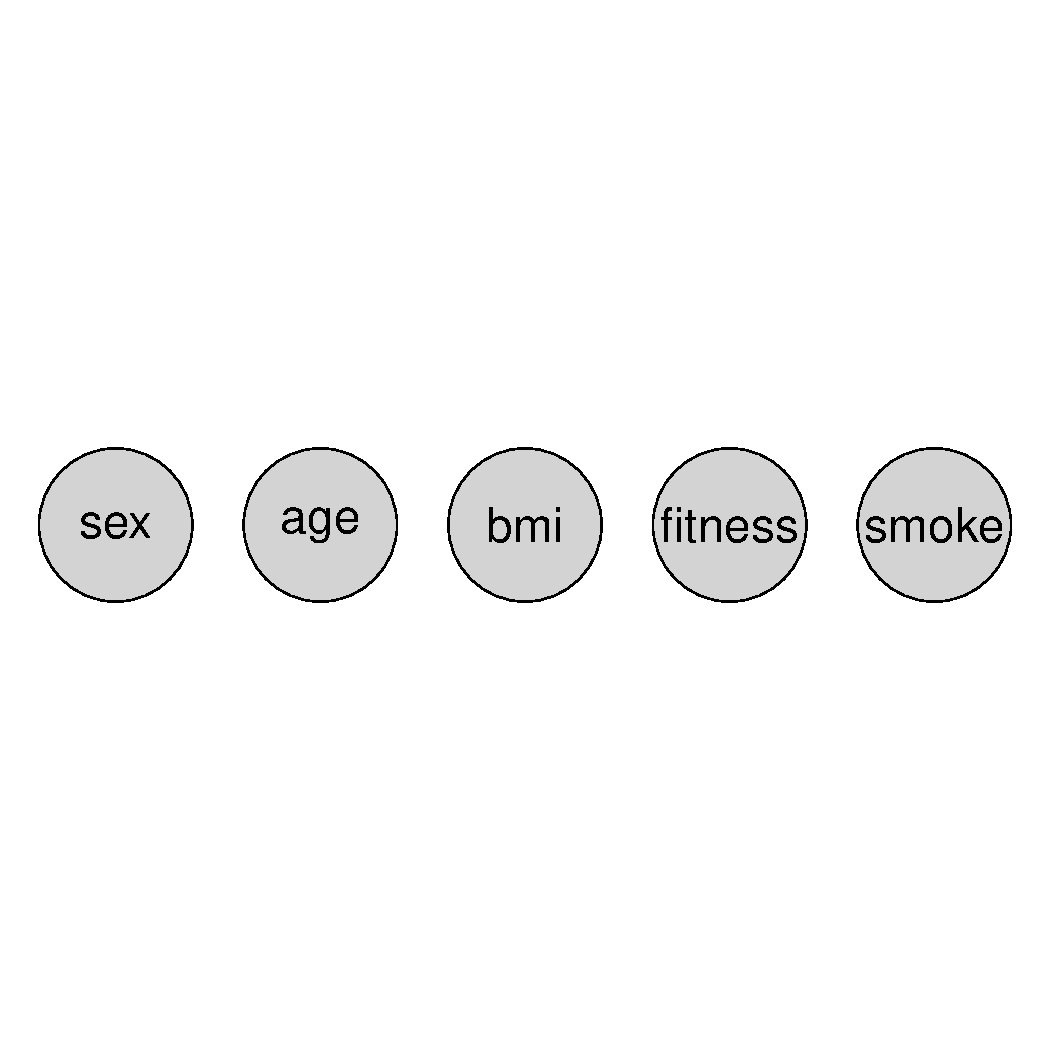
\includegraphics[width=\maxwidth]{figure/VisualizzazioneGrafoModello-1} 
\end{knitrout}

\clearpage


\clearpage

\section{Modelli Grafi}
  \subsection{Tabella Frequenze}
\begin{knitrout}
\definecolor{shadecolor}{rgb}{0.969, 0.969, 0.969}\color{fgcolor}\begin{kframe}
\begin{alltt}
\hlcom{#Tabella}
\hlkwd{ftable}\hlstd{(sex}\hlopt{+}\hlstd{bmi}\hlopt{+}\hlstd{pa} \hlopt{~} \hlstd{smoke}\hlopt{+}\hlstd{alc}\hlopt{+}\hlstd{fitness, nmc)}
\end{alltt}
\begin{verbatim}
##                     sex Female                Male               
##                     bmi      0         1         0         1     
##                     pa       0    1    0    1    0    1    0    1
## smoke   alc fitness                                              
## Current 1   1                4    1    1    0    2    1    0    1
##             2               11    6    6    0    3    2    2    0
##             3               31    1    3    0    8    2    1    0
##             4                6    1    0    0    3    0    0    0
##             5                5    0    0    0    4    0    0    0
##         2   1               26    8   12    3    6    3    4    2
##             2              166   44   25    9   26    6    2    1
##             3              449   37   21    1   94   10    5    1
##             4              193    4    8    1   52    1    1    0
##             5               55    0    2    0   18    1    0    0
##         3   1               11    8    6    2   10    6    2    1
##             2               74   21   16    3   49   15    2    2
##             3              287   32   14    3  156   24   11    0
##             4              200    8    5    0  129    4    3    0
##             5               49    0    2    0   32    0    0    0
##         4   1                0    0    0    2    0    2    0    0
##             2                4    1    0    0    5    0    1    0
##             3               12    3    1    0   17    0    1    0
##             4                9    1    1    0    7    0    1    0
##             5                8    0    0    0    6    1    0    0
## Former  1   1                2    4    6    3    2    2    0    1
##             2               16    5   10    2    7    4    0    2
##             3               83   14   17    1   42    1    6    0
##             4               63    0    8    0   32    5    3    0
##             5               35    0    0    0   15    0    0    0
##         2   1               35   18   17   12    9    8    8    4
##             2              185   41   70   12   39   16   12    3
##             3             1005   70  124    8  279   40   27    5
##             4              799   24   33    0  348   14   16    0
##             5              290    1    3    1  140    0    4    1
##         3   1               11    7    9    8    9    5    6    5
##             2              132   26   27    8   94   34   30   14
##             3              846   81   57    6  563   57   47   11
##             4              829   15   22    2  740   24   34    2
##             5              281    2    3    0  308    2    6    0
##         4   1                3    0    0    0    2    1    0    0
##             2                4    0    0    0    3    2    0    0
##             3               39    2    3    0   45    7    6    2
##             4               28    2    1    0   60    2    5    0
##             5               14    0    0    0   24    0    0    0
## NO      1   1               30   13   21   10   10    3    1    1
##             2              209   38   49   10   68   22   10    1
##             3             1024   83  111    9  272   30   15    1
##             4              704   19   44    0  386   21    6    1
##             5              255    1    9    0  194    4    2    0
##         2   1               81   28   38   13   29    8    9    6
##             2              624  132  139   20  192   55   26   14
##             3             3169  258  246   18  805   92   48    4
##             4             2549   49   80    3 1059   36   19    1
##             5              876    6   21    0  628   12    3    1
##         3   1               24    9   14    4   21   10    7    3
##             2              212   42   41    9  124   48   23    5
##             3             1288  109   82   11  715  101   40    9
##             4             1326   29   36    2 1093   35   29    0
##             5              441    4    4    0  577    6    6    0
##         4   1                3    0    0    0    3    2    0    0
##             2                1    2    2    0    9    5    4    0
##             3               35    5    2    0   45    5    5    0
##             4               48    0    1    0   53    6    4    0
##             5               14    0    0    0   47    0    1    0
\end{verbatim}
\end{kframe}
\end{knitrout}
    
\begin{knitrout}
\definecolor{shadecolor}{rgb}{0.969, 0.969, 0.969}\color{fgcolor}\begin{kframe}
\begin{alltt}
\hlcom{#Dataset per grafi}
\hlstd{nmc.nocvd} \hlkwb{<-} \hlstd{nmc[}\hlkwd{c}\hlstd{(}\hlnum{1}\hlopt{:}\hlnum{3}\hlstd{,} \hlnum{5}\hlopt{:}\hlnum{8}\hlstd{)]}
\hlstd{nmc.cvd0} \hlkwb{<-} \hlstd{nmc[(nmc}\hlopt{$}\hlstd{cvd}\hlopt{==}\hlnum{0}\hlstd{),}\hlkwd{c}\hlstd{(}\hlnum{1}\hlopt{:}\hlnum{3}\hlstd{,} \hlnum{5}\hlopt{:}\hlnum{8}\hlstd{)]}
\hlstd{nmc.cvd1} \hlkwb{<-} \hlstd{nmc[(nmc}\hlopt{$}\hlstd{cvd}\hlopt{==}\hlnum{1}\hlstd{),}\hlkwd{c}\hlstd{(}\hlnum{1}\hlopt{:}\hlnum{3}\hlstd{,} \hlnum{5}\hlopt{:}\hlnum{8}\hlstd{)]}
\end{alltt}
\end{kframe}
\end{knitrout}
    
  \subsection{Grafi}
\begin{knitrout}
\definecolor{shadecolor}{rgb}{0.969, 0.969, 0.969}\color{fgcolor}\begin{kframe}
\begin{alltt}
\hlcom{#Modello scelto}
\hlstd{m.fit} \hlkwb{<-} \hlkwd{dmod}\hlstd{(}\hlopt{~}\hlstd{sex}\hlopt{+}\hlstd{age}\hlopt{+}\hlstd{bmi}\hlopt{+}\hlstd{fitness}\hlopt{+}\hlstd{smoke,} \hlkwc{data}\hlstd{=nmc,} \hlkwc{fit}\hlstd{=}\hlnum{TRUE}\hlstd{)}
\hlstd{m.fit}
\end{alltt}
\begin{verbatim}
## Model: A dModel with 5 variables
##  -2logL    :      466894.73 mdim :   82 aic :    467058.73 
##  ideviance :           0.00 idf  :    0 bic :    467748.69 
##  deviance  :       11626.84 df   : 4417
\end{verbatim}
\begin{alltt}
\hlkwd{plot}\hlstd{(m.fit)}
\end{alltt}
\end{kframe}
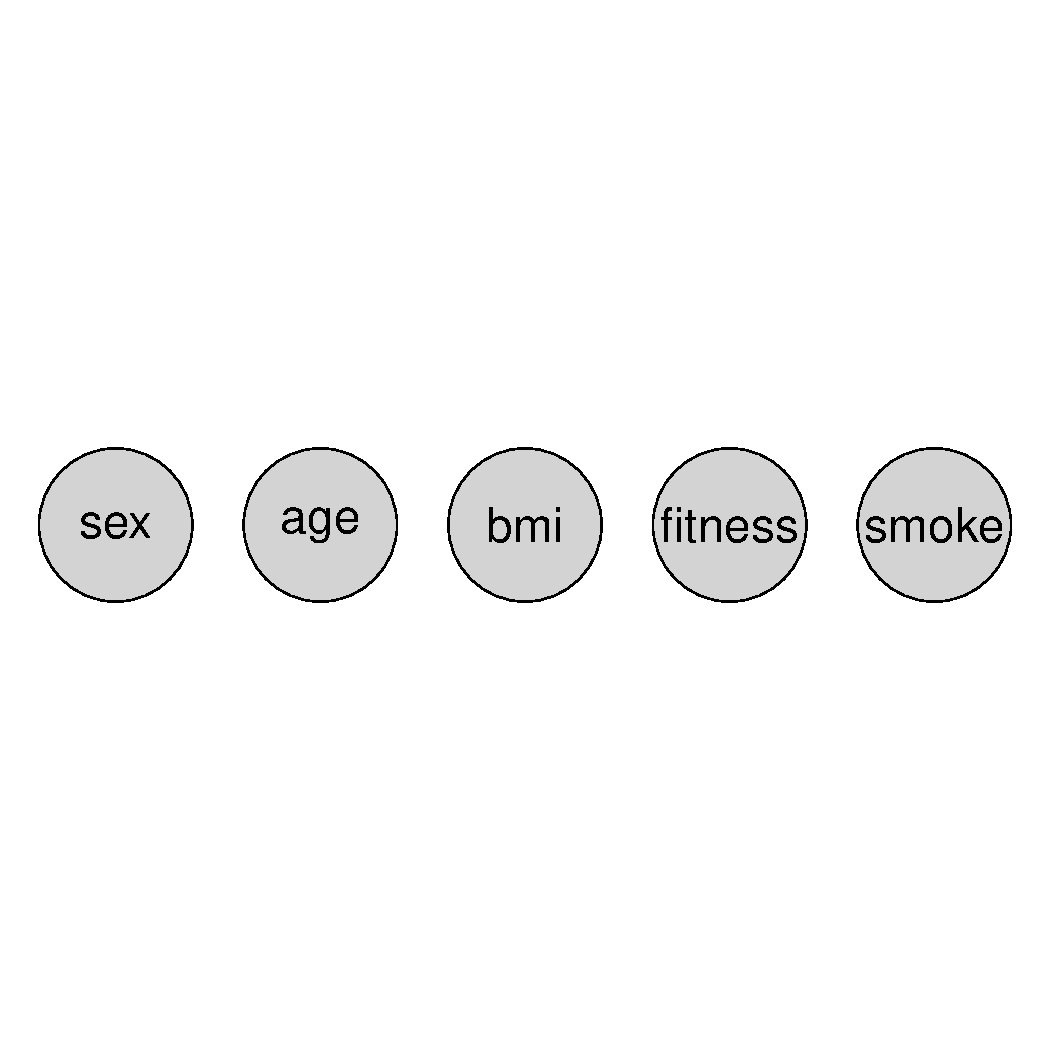
\includegraphics[width=\maxwidth]{figure/Modello_scelto-1} 
\end{knitrout}
    
\begin{knitrout}
\definecolor{shadecolor}{rgb}{0.969, 0.969, 0.969}\color{fgcolor}\begin{kframe}
\begin{alltt}
\hlcom{#Formula modello saturo}
\hlstd{sat.nmc.cvd0} \hlkwb{<-} \hlkwd{dmod}\hlstd{(}\hlopt{~}\hlstd{.}\hlopt{^}\hlstd{.,} \hlkwc{data}\hlstd{=nmc.cvd0)}
\hlstd{sat.nmc.cvd1} \hlkwb{<-} \hlkwd{dmod}\hlstd{(}\hlopt{~}\hlstd{.}\hlopt{^}\hlstd{.,} \hlkwc{data}\hlstd{=nmc.cvd1)}
\end{alltt}
\end{kframe}
\end{knitrout}
\begin{knitrout}
\definecolor{shadecolor}{rgb}{0.969, 0.969, 0.969}\color{fgcolor}\begin{kframe}
\begin{alltt}
\hlcom{#Formula modello indipendenza completa}
\hlstd{ind.nmc.cvd0} \hlkwb{<-} \hlkwd{dmod}\hlstd{(}\hlopt{~}\hlstd{.}\hlopt{^}\hlnum{1}\hlstd{,} \hlkwc{data}\hlstd{=nmc.cvd0)}
\hlstd{ind.nmc.cvd1} \hlkwb{<-} \hlkwd{dmod}\hlstd{(}\hlopt{~}\hlstd{.}\hlopt{^}\hlnum{1}\hlstd{,} \hlkwc{data}\hlstd{=nmc.cvd1)}
\end{alltt}
\end{kframe}
\end{knitrout}
    
\begin{knitrout}
\definecolor{shadecolor}{rgb}{0.969, 0.969, 0.969}\color{fgcolor}\begin{kframe}
\begin{alltt}
\hlcom{#AIC}
\hlstd{m.sat.cvd0} \hlkwb{<-} \hlkwd{stepwise}\hlstd{(sat.nmc.cvd0)}
\hlkwd{plot}\hlstd{(m.sat.cvd0)}
\end{alltt}
\end{kframe}
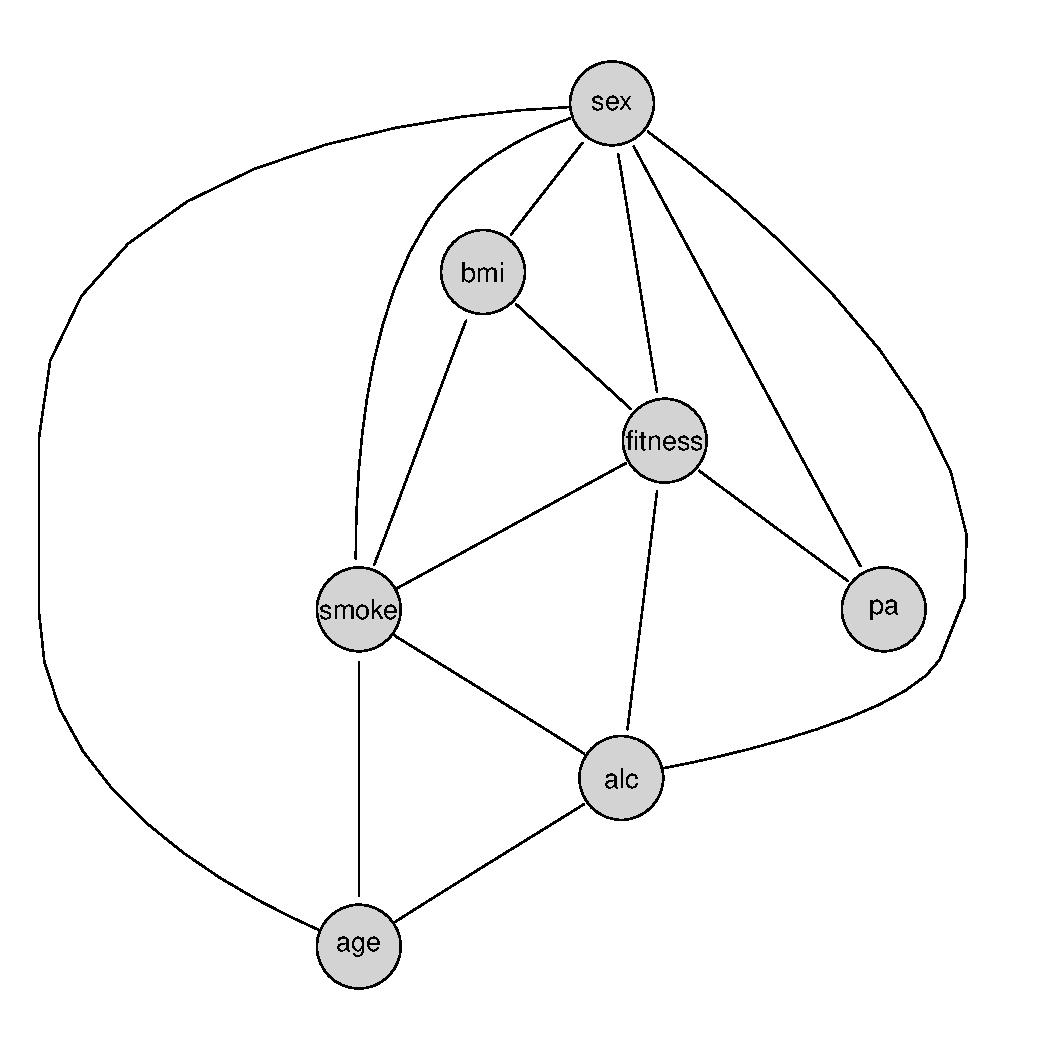
\includegraphics[width=\maxwidth]{figure/Grafo_AIC_CVD0-1} 
\end{knitrout}
    
\begin{knitrout}
\definecolor{shadecolor}{rgb}{0.969, 0.969, 0.969}\color{fgcolor}\begin{kframe}
\begin{alltt}
\hlcom{#AIC}
\hlstd{m.sat.cvd1} \hlkwb{<-} \hlkwd{stepwise}\hlstd{(sat.nmc.cvd1)}
\hlkwd{plot}\hlstd{(m.sat.cvd1)}
\end{alltt}
\end{kframe}
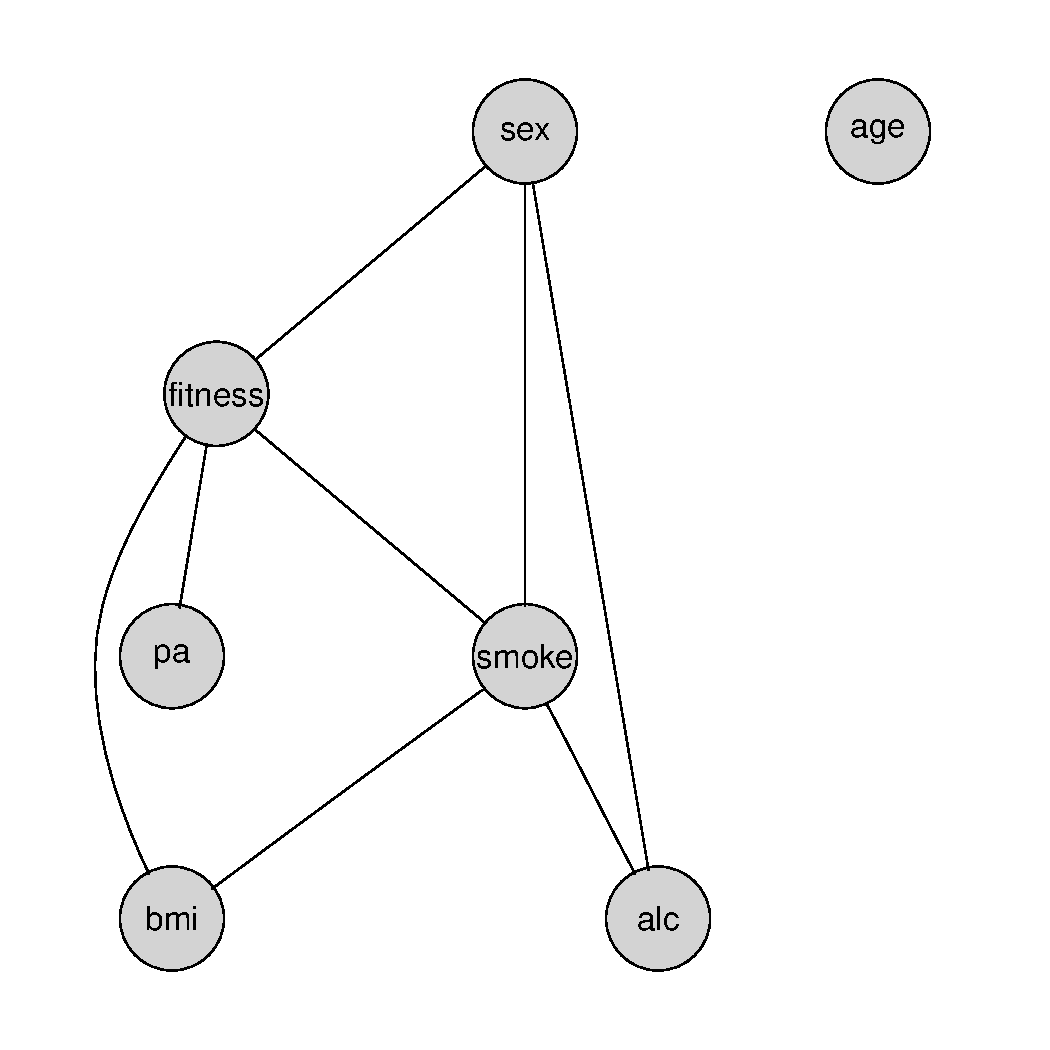
\includegraphics[width=\maxwidth]{figure/Grafo_AIC_CVD1-1} 
\end{knitrout}
    
\begin{knitrout}
\definecolor{shadecolor}{rgb}{0.969, 0.969, 0.969}\color{fgcolor}\begin{kframe}
\begin{alltt}
\hlcom{#BIC}
\hlstd{m.ind.cvd0} \hlkwb{<-} \hlkwd{stepwise}\hlstd{(ind.nmc.cvd0,} \hlkwc{k}\hlstd{=}\hlkwd{log}\hlstd{(}\hlkwd{length}\hlstd{(nmc}\hlopt{$}\hlstd{cvd)),}
                       \hlkwc{direction}\hlstd{=}\hlstr{"forward"}\hlstd{)}
\hlkwd{plot}\hlstd{(m.ind.cvd0)}
\end{alltt}
\end{kframe}
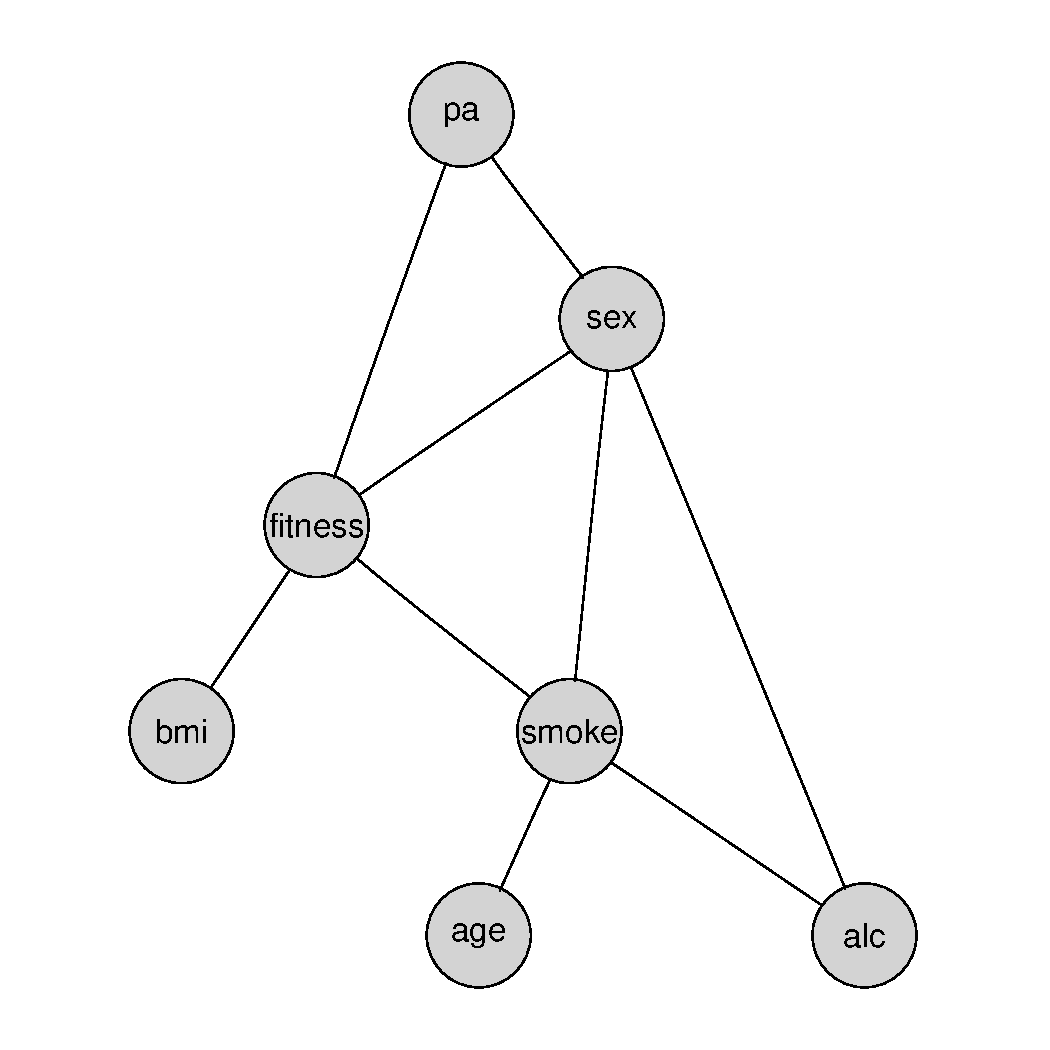
\includegraphics[width=\maxwidth]{figure/Grafo_BIC_CVD0-1} 
\end{knitrout}
    
\begin{knitrout}
\definecolor{shadecolor}{rgb}{0.969, 0.969, 0.969}\color{fgcolor}\begin{kframe}
\begin{alltt}
\hlcom{#BIC}
\hlstd{m.ind.cvd1} \hlkwb{<-} \hlkwd{stepwise}\hlstd{(ind.nmc.cvd1,} \hlkwc{k}\hlstd{=}\hlkwd{log}\hlstd{(}\hlkwd{length}\hlstd{(nmc}\hlopt{$}\hlstd{cvd)),}
                       \hlkwc{direction}\hlstd{=}\hlstr{"forward"}\hlstd{)}
\hlkwd{plot}\hlstd{(m.ind.cvd1)}
\end{alltt}
\end{kframe}
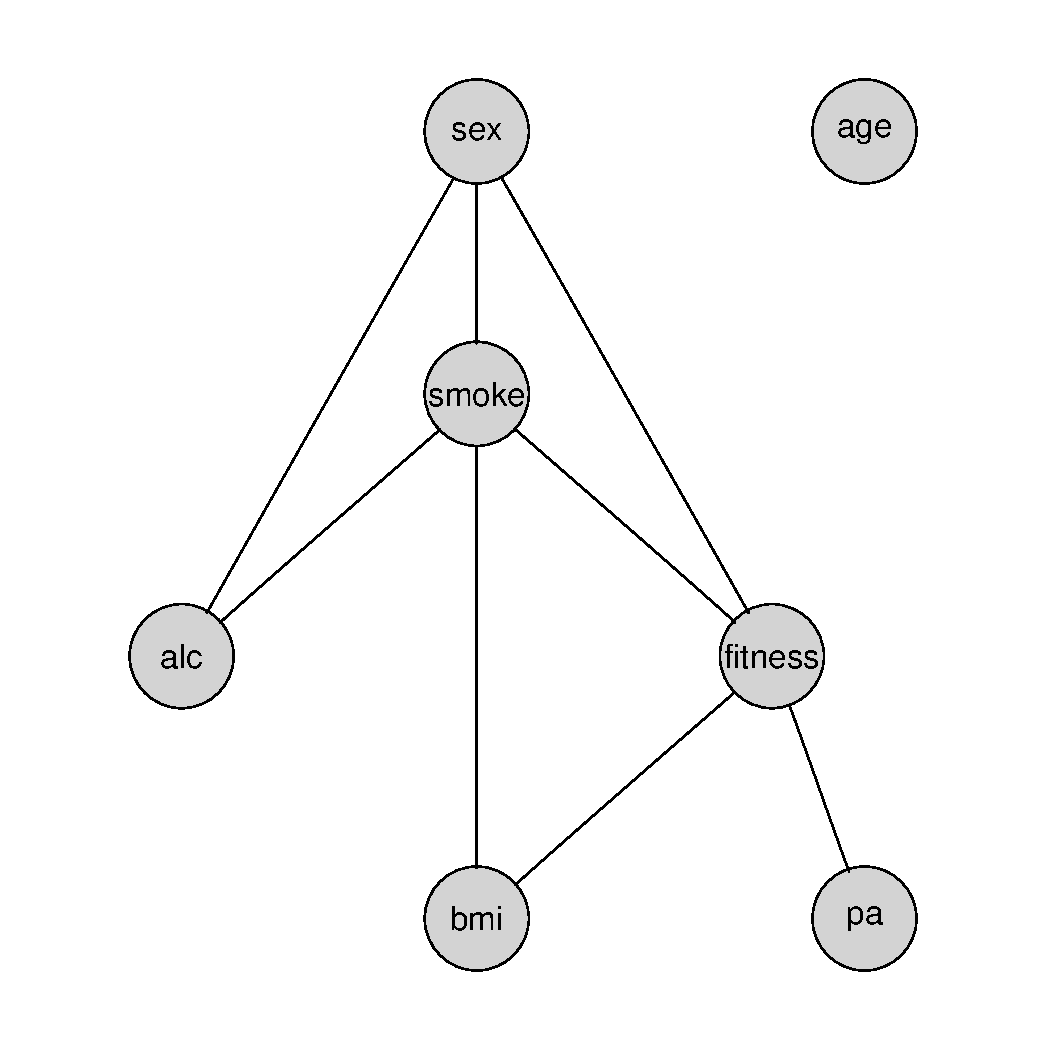
\includegraphics[width=\maxwidth]{figure/Grafo_BIC_CVD1-1} 
\end{knitrout}


\section{Conclusioni}
  In conclusione, il modello scelto che più si adatta meglio al problema per il 
  calcolo della probabilità di un problema cardiovascolare è:\\
  Modello: CVD $\sim$ Sex + Age + BMI + Fitness + Smoke. \par
  All'interno del modello sono presenti unicamente variabili significative e
  indipendenti.\par
  I fattori che aumentano la probabilità di CVD sono:
  \begin{itemize}
    \item L'aumento dell'età, con maggior evidenza superati i 40 anni.
    \item Essere maschio.
    \item Essere un fumatore.
    \item Avere un alto indice di massa corporea.
  \end{itemize}
  I fattori che non influenzano la CVD sono:
  \begin{itemize}
    \item Il consumo di alchol.
    \item La tipologia di attività fisica.
  \end{itemize}
  E' stato scelto questo modello a differenza di altri modelli (come il modello 
  con interazioni) perchè rappresenta al meglio lo studio svolto sulle varie
  categorie e contemporaneamente risulta essere un modello abbastanza semplice e
  significativo.

\end{document}
